\documentclass[a4paper,12pt]{book}
\usepackage[english]{babel}
\usepackage[utf8]{inputenc}
\usepackage[T1]{fontenc}
\usepackage{lmodern}
\usepackage{graphicx}
\usepackage{amsmath}
\usepackage{amsfonts}
\usepackage{amssymb}
\usepackage{amsthm}
\usepackage{multirow}
\usepackage{physics}
\usepackage{enumerate}
%\usepackage{xr-hyper}
\usepackage{hyperref}
\usepackage{fancyhdr}
\usepackage[super]{nth}
\usepackage[margin=1in]{geometry}
%\usepackage{units}	% To use \nicefrac
\usepackage[nottoc,notlot,notlof]{tocbibind}	% Include Bibliography in Table of Contents unnumbered 

\hypersetup{
	%hidelinks,		% Remove ugly borders around clickable cross-references and hyperlinks
	linktoc=all,     % set to all if you want both sections and subsections linked
	%colorlinks=true, % set true if you want colored links
	%linkcolor=blue,  %choose some color if you want links to stand out
}

% Header format
\geometry{headheight=15pt}
\pagestyle{fancy}
\fancyhf{} % to clear existing header/footer if you don't want it
\fancyhead[LE,RO]{\thepage}
\fancyhead[LO]{\rightmark}
\fancyhead[RE]{\leftmark}
\let\MakeUppercase\relax	% Header not in uppercase

\interfootnotelinepenalty=10000

\def\labelitemi{--}

\theoremstyle{plain}
\newtheorem{theorem}{Theorem}[chapter]
\newtheorem{proposition}[theorem]{Proposition}
\newtheorem{corollary}[theorem]{Corollary}
\newtheorem{lemma}[theorem]{Lemma}

\theoremstyle{definition}
\newtheorem{definition}[theorem]{Definition}
\newtheorem{example}[theorem]{Example}
\newtheorem{task}[theorem]{Task}
\newtheorem{hypothesis}[theorem]{Hypothesis}

\theoremstyle{remark}
\newtheorem{remark}[theorem]{Remark}

\begin{document}

\author{Raul Murillo Montero}
\title{Qualitative Theory of Ordinary Differential Equations\\
\Large   Notes from Henryk Żoł\c{a}dek\\
\large   Version 1.0}
\date{October 2017}

\frontmatter
\begin{titlepage}
	\hbox{
		\hspace*{0.1\textwidth} % Whitespace to the left of the title page
		\rule{1pt}{\textheight} % Vertical line
		\hspace*{0.05\textwidth} % Whitespace between the vertical line and title page text
		\parbox[b]{0.75\textwidth}{ % Paragraph box which restricts text to less than the width of the page
			%{\noindent\Huge\bfseries Trabalho de Cálculo \\}\\[0.01\baselineskip] % Title
			
			
			%----------------------------------------------------------------------------------------
			%	TITLE SECTION
			%----------------------------------------------------------------------------------------
			{\Large Applied mathematics}\\[1.5cm] % Major heading such as course name
			% Minor heading such as course title
			{ \Huge  \bfseries Qualitative Theory of\\Ordinary Differential\\
			Equations}\\[2cm] % Title of your document
			
			%----------------------------------------------------------------------------------------
			%	AUTHOR SECTION
			%----------------------------------------------------------------------------------------			
			
			\begin{minipage}[t]{0.4\textwidth}
				\begin{flushleft} \large
					Raul Murillo Montero\\% Your name
					7th Semester\\
					Universidad Complutense de Madrid\\
					[1\baselineskip]
					\includegraphics[scale=0.55]{UCM.png} % Include a department/university logo - this will require the graphicx package
				\end{flushleft}
			\end{minipage}
			~
			\begin{minipage}[t]{0.4\textwidth}
				\begin{flushright} \large
					Mr. Henryk Żoł\c{a}dek\\Prof. dr. hab.\\% Supervisor's Name
					Uniwersytet Warszawski\\
					[2\baselineskip]
					\includegraphics[scale=0.4]{UW.png} % Include a department/university logo - this will require the graphicx package
				\end{flushright}
			\end{minipage}\\[1cm]
			
			\vspace{0.25\textheight} % Whitespace between the title block and the publisher
			{\noindent University of Warsaw, 2018 }\\[\baselineskip] % Publisher and logo
		}
		}
	
	\vfill % Fill the rest of the page with whitespace
	
\end{titlepage}
\tableofcontents

\mainmatter
\chapter*{Introduction}
\addcontentsline{toc}{chapter}{Introduction}

The Qualitative Theory of Ordinary Differential Equations takes a rather special place both in Applied Mathematics and in theoretical Mathematics. On the one hand, it is a continuation of the standard lecture on Ordinary Differential Equations (ODEs). On the other hand, it is an introduction to the theory of Dynamical Systems, one of the main mathematical disciplines in recent decades. In addition, it turns out to be very useful for graduates when they meet with differential equations at work, which are usually very complicated and can not be solved by standard methods. If I do not boast too much, the first lecture from Qualitative Theory of ODEs at the Faculty of MIM was made by me in the second half of the 80s of the last century; as you can see, the idea turned out to be successful.

The main idea of a qualitative analysis of differential equations is that without solving the equations themselves, be able to say something about the behavior of solutions.

Therefore, in the first place stand out certain properties such as the stability of solutions. It is stable with respect to changes in the initial conditions of the equation. Note that even with the numerical approach to differential equations all the calculations are subject to certain inevitable error. Therefore, it is good when the asymptotic behavior of the solutions is sensitive to perturbations of the initial state. The first part of the script focuses on this roughly.

Another important concept of this theory is the structural stability. This is the stability of the entire system, i.e. the phase portrait, with regard to perturbation parameters, which usually occur (and in large quantities) on the right side of the equations. In the absence of structural stability, we deal with bifurcations. Methods of qualitative theory allow for precise and accurate enough to examine such bifurcations. We describe them in the third part of the script.

In the case of 2-dimensional autonomous systems, the phase portraits are conceptually quite simple, they consist of singular points, their separatrices and limit cycles;  there are still the peculiarities and blow behavior on the infinite. It is worth mentioning that the problem of limit cycles for polynomial vector fields is the unresolved Hilbert's sixteenth problem. These topics are discussed in the second part of the script.

The fourth part is dedicated to several issues in which there is a small parameter (in a different context). In particular, this class of issues includes the KAM theory and the theory of relaxation oscillations; we discuss them fairly briefly.

In multidimensional systems, new phenomena appear, of which the most important is chaos. The most elementary example of a chaotic system is the famous Smale horseshoe map, defined for a single transformation. In the penultimate part of this script, we will show how Smale horseshoe appears in such elementary systems as a swing moved by periodic external force. We will also give other examples of chaotic behaviors, as attractors.

In the Appendix (Chapter 6), the reader will find the collected main facts from the course lecture on Ordinary Differential Equations.

Each chapter contains a series of tasks (with varying degrees of difficulty) that a self-respecting student should solve.

At the end of the introduction, I would like to thank Professor Zbigniewowi Peradzyńskiemu, who carefully read the manuscript and gave me a list of comments and errors.\\

\begin{flushright}
	Henryk Żoł\c{a}dek,\\
	University of Warsaw,\\
	Faculty of Mathematics, Informatics, and Mechanics, 2011	
\end{flushright}
\chapter{Vector field equilibrium points}

Let's consider the non-autonomous system of differential equations (or time-dependent vector field)
\begin{equation}\label{1.1}
	\dot{x} = v (t, x).
\end{equation}
Here $x$ belongs to a certain variety $M$ and $t$ (time) to an interval $I\subset \mathbb{R}$. In this chapter we can assume that $M$ is an open subset $\mathbb{R}^n$ and that the field $v$ is of class $C^r,$ $r\geq 2$; so that the assumptions of the Appendix are fulfilled.

Recall that a point $x_*$ such that,
$$
v(t,x_{\ast })=0
$$
(for every $t$) is called \textbf{equilibrium point}; other names in the literature are:
\textbf{singular point} and \textbf{critical point} of the field (mainly in the case of an autonomous fields).
Of course, $\varphi(t) \equiv x_*$ is the solution to this problem. The purpose of this chapter is to examine the
properties of the solution of the system \eqref{1.1} in the neighborhood of the equilibrium point.

\section{Stability in the Lyapunov sense and asymptotic stability}
The simplest and desired property from the point of view of the use of the equilibrium point is its stability. Below are two mathematically strict definitions of stability.
\begin{definition}\label{def:1.1}
	An equilibrium point $x_*$ of equation \eqref{1.1} is \textbf{stable in the Lyapunov sense}, if, for every $\varepsilon > 0$, there exists a $\delta > 0$ such that, if $\left|x_0-x_* \right| < \delta$, then for every time $t> t_0$ we have $\left|\varphi(t;x_0,t_0) - x_* \right| < \varepsilon$.
		
	An equilibrium point $x_*$ is \textbf{asymptotically stable} if it is stable in the Lyapunov sense and, in addition, there exists $\varepsilon_0 > 0$ such that if $\left|x_0-x_* \right| < \varepsilon_0$, then $\lim \varphi(t;x_0,t_0) = x_*$ when $t \to \infty$.
\end{definition}

\begin{example}
	For the \textit{harmonic oscillator} $\ddot{x} = - \omega^2-x$, or
	$$\dot{x} = y,\ \dot{y} =  - \omega^2-x$$
	the solutions lie in the ellipses $\{ (\omega x)^2 + y^2 = \varepsilon^2 \}$ (see Figure \ref{fig:1.1}). The fact that $0 < \omega \leq 1$ shows that the product $\delta = \omega \varepsilon$ satisfies the definition of stability in the Lyapunov sense. Since the solution does not reach the equilibrium point $x = y = 0$, it is not asymptotically stable.
\end{example}

\begin{figure}[!ht]
	%\vspace{-15pt}
	\centering
	\includegraphics[scale=1.4]{jtr11}
	\caption{Harmonic oscillator.}
	%\vspace{-10pt}
	\label{fig:1.1}
\end{figure}

\begin{example}
	Figure \ref{fig:1.2} shows a phase portrait of a vector field that has the property that each solution reaches the equilibrium point (i.e. the second of the conditions for asymptotic stability is fulfilled). However, this equilibrium point is not stable in the Lyapunov sense, since the trajectories starting from the bottom and arbitrarily close to the equilibrium point emerge over time from the fixed environment of this point.
	
	It turns out that the appropriate autonomous vector field can be specified by a specific pattern. Namely, it has the form
	\begin{equation}\label{1.2}
		\dot{x} = y, \ \dot{y} = -2x^3-4xy-y(x^2+y^2)^2
	\end{equation}
	(see Task 2.64).
\end{example}

\begin{figure}[!ht]
	%\vspace{-15pt}
	\centering
	\includegraphics [scale=1.5]{jtr12}
	\caption{Not Lyapunov stable.}
	%\vspace{-10pt}
	\label{fig:1.2}
\end{figure}

The main result of the stability of equilibrium points is from A. Lyapunov. It concerns the equilibrium point $x = 0$ for the germ\footnote{By the vector field germ $v (x)$ (or the function $f (x)$ or the differential form $w(x)$ or mapping) at point $x_0\in \mathbb{R}^n$ we mean a vector field (or function or differential form or mapping) defined on a certain neighborhood $U$ of point $x_0$. Two germs, one defined on a neighborhood $U$ and the other an $U'$, are equivalent if they are compatible in a certain neighborhood $V \subset U \cap U'$. The notation $f: (\mathbb{R}^n, x_0)\to \mathbb{R}$ is used to denote the germ of the function in $x_0$; analogous notations are for vector fields, differential forms, mappings, etc.} of an autonomous vector field in $(\mathbb{R}^n, 0)$ of the form
\begin{equation}\label{1.3}
	v(x) = Ax + O(\left|x\right|^2),
\end{equation}
where $A = \frac{\partial v}{\partial x}(0)$ is the linearization matrix of the field at $x = 0$.

\begin{theorem}\label{theo:1.4}
	\emph{(Lyapunov).}
	If the linearization matrix A has the property that the real parts of all its eigenvalues are negative,
	\begin{equation}\label{eq:Lyapunov}
		\Re \lambda_j <0,
	\end{equation}
	the equilibrium point $x = 0$ is asymptotically stable.
\end{theorem}

Before we begin the strict proof this theorem, we introduce the concept of Lyapunov function, which turns out to be useful for showing asymptotic stability even without assumption \eqref{eq:Lyapunov}.

\begin{definition}\label{def:Lyap_funct}
	A \textbf{Lyapunov function} for the equilibrium point $x = 0$ of the autonomous vector field $v(x)$ is a function
	$$L: U \to \mathbb{R}$$
	from the neighborhood $U$ of the point $x = 0$, which satisfies the following two properties:
	\begin{enumerate}[(i)]
		\item $L(x) \geq 0$ and $L(x) = 0$ iff $x=0$;
		\item $\dot{L}(x) = \left\langle dL(x), v(x) \right\rangle < 0$ for $x \neq 0$.
	\end{enumerate}
\end{definition}

\begin{proposition}\label{prop:asymp_stable}
	If there is a Lyapunov function (for the equilibrium point $x = 0$ of the field $v(x)$) then this point is asymptotically stable.
	\begin{proof}
		The property (i) from the definition of the Lyapunov function says that the sets $\left\lbrace L(x) \leq c \right\rbrace$, $c> 0$, are bounded and tend to the point $x = 0$ at $c \to 0$.
		
		Property (ii) means that if $x = \varphi(t)$ is the solution of equation $\dot{x} = x(x)$, then
		$$\frac{d}{dt} L \circ \varphi(t) = \frac{\partial L}{\partial x}(\varphi(t))\cdot\dot{\varphi}(t) = \left(\nabla L(x), v(x) \right) = \left\langle dL(x), v(x) \right\rangle < 0.$$
		It can be seen that the Lyapunov function decreases along the solutions of the differential equation (see Figure \ref{fig:Lyapunov_funct}).
		
		So the solutions starting from the boundary $\{L (x) = c\}$ of the set $\{L (x) \leq c\}$ `enter' into the interior of this set. Since these trajectories remain in the sets $\{L\leq c\}$, the condition of stability in the Lyapunov sense is satisfied. On the other hand, the solution must reach point $x = 0$ at $t\to \infty$; and this means asymptotic stability.
	\end{proof}
\end{proposition}

\begin{figure}[!ht]
	%\vspace{-15pt}
	\centering
	\includegraphics[scale=1.4]{jtr13} 
	\caption{Lyapunov function.}
	%\vspace{-10pt}
	\label{fig:Lyapunov_funct}
\end{figure}

Now, for the proof of Lyapunov's theorem, it is necessary to construct the Lyapunov functions. For this purpose, we will slightly improve the $A$ matrix. First of all, we assume that it is in the Jordan form. So we have blocks
$$ \begin{pmatrix}
\lambda_j & 1 & 0 & \ldots & 0 & 0\\ 
0& \lambda_j & 1 & \ldots & 0 & 0\\ 
\vdots& \vdots & \vdots & \ddots & \vdots & \vdots\\ 
0& 0 & 0 & \ldots & \lambda_j & 1\\ 
0& 0 & 0 & \ldots & 0 & \lambda_j
\end{pmatrix},\ \begin{pmatrix}
\alpha_j & -\beta_j & 1 & 0 & \ldots\\ 
\beta_j& \alpha_j & 0 & 1 & \ldots\\ 
0 &0  & \alpha_j & -\beta_j & \ldots\\ 
0 & 0 & \beta_j & \alpha_j & \ldots\\ 
\ldots & \ldots & \ldots & \ldots & \ldots
\end{pmatrix},$$
corresponding to unreal ($\lambda_1$, \dots, $\lambda_r$) and complex ($\lambda_j = \bar{\lambda}_{j+1} = \alpha_j+ i\beta_j$, $j = r+1$, $r+3$, \dots, $n-1$) eigenvalues.

It turns out that the ones over the diagonal can be replaced with small $\varepsilon$. Actually, if we have a Jordan $k$-dimension block with the real value of $\lambda$, then in the standard base ($e_j$) we have
$$Ae_1 = \lambda e_1,\ Ae_2 = \lambda e_2 + e_1, \ldots,\ Ae_k = \lambda e_k + e_{k-1}.$$
So for base ($f_j$) such that
$$f_k = e_k,\ f_{k-1} = \frac{e_{k-1}}{\varepsilon}, \ldots,\ f_1 = \frac{e_1}{\varepsilon^{k-1}},$$
we will have $Af_1 = f_1$ and $Af_j = \lambda f_j + \varepsilon f_{j-1}$ ($j>1$). We use analogue conversions when we have a Jordan block with complex eigenvalues (Task 1.27). So we have the following

\begin{lemma}\label{lemma:1.7}
	There exists a linear coordinate system such that matrix $A$ takes the form
	$$A = A_0 + \varepsilon A_1$$
	where $A_0$ is block-diagonal with $\lambda_j \in \mathbb{R}$ or $\begin{pmatrix}
	\alpha_j & -\beta_j \\ 
	\beta_j& \alpha_j \\ \end{pmatrix}$ on diagonals and the matrix $A_1$ is bounded, $\left\|A_1\right\|<C_1$.
\end{lemma}

Next lemma concludes the proof of Theorem \ref{theo:1.4}
\begin{lemma}\label{lemma:2}
	Let $(x_i)$ be the coordinate system from Lemma \ref{lemma:1.7} thesis. Then the function
	$$L(x) = \sum x_i^2 = (x,x) = \left|x\right|^2$$
	in a suitably small neighborhood of the point $x= 0$ is a Lyapunov function for this equilibrium point.
	\begin{proof}
		Of course, we only need to check property (ii) from Definition \ref{def:Lyap_funct} of Lyapunov function. We have
		$$\dot{L} = (\nabla L, A_0x) + \varepsilon(\nabla L, A_1x) + (\nabla L, v-Ax),$$
		where $\nabla L = 2x$. The first member to the right of this equality is (how easy it is to check)
		\begin{equation}\label{eq:lemma_eq}
			(\nabla L, A_0x) = 2\sum_{j=1}^{r}\lambda_j x_j^2 + 2\sum \alpha_j(x_j^2+x_{j+1}^2),
		\end{equation}
		where in the second sum we sum $j = r + 1$, $r + 3$,\dots, $n - 1$. Then, with the $A_1$ bound we get
		$$\left|(\nabla L, A_1x)\right| \leq 2C_1\left|x\right|^2.$$
		Since the nonlinear terms $v (x) - Ax$ are of the form $O (\left|x\right| ^2)$, we have
		$$\left|(\nabla L, v-Ax)\right| \leq 2C_2\left|x\right|^3 \leq 2C_2\varepsilon \left|x\right|^2$$
		for a certain constant $C_2$ and sufficiently small $\left|x\right|$.
		
		The condition \eqref{eq:Lyapunov} from the assumption of Lyapunov's theorem means that in \eqref{eq:lemma_eq} we have
		$$\lambda_j, \alpha_k < - \Lambda < 0$$
		for certain $\Lambda$. So we have $(\nabla L, A_0x) < -2\Lambda \left|x\right|^2$ and the other two members in $\dot{L}$ are estimated by $2(C_1+C_2) \varepsilon \left|x\right|^2$. This shows that $\dot{L} <0$ for $x \neq 0$ and small $\varepsilon$, which concludes the proof of lemma and Lyapunov's theorem.
	\end{proof}
\end{lemma}

There is a theorem opposite to Lyapunov's theorem. It is quite natural and presumably Lyapunov had his consciousness, but in Russian literature (e.g. in \cite{Fil}) it is attributed to V. Chetaev.

\begin{theorem}\emph{(Chetaev).}
	If the linearization matrix $A$ of the vector field \eqref{1.3} has an eigenvalue with positive real part, then the equilibrium point $x = 0$ is not stable (neither in Lyapunov sense nor asymptotically).
	\begin{proof}
		Let $\Re \lambda_1,\ldots, \Re \lambda_k > 0$ and $\Re \lambda_{k+1}, \ldots, \Re \lambda_{k+l} \leq 0$, $n = k+l$. We can assume that
		$$A = A_1 \oplus A_2$$
		in the distribution $\mathbb{R}^n = \mathbb{R}^k \oplus \mathbb{R}^l$, where the matrix $A_1$ has the eigenvalues $\lambda_1,\ldots, \lambda_k$ and the matrix $A_2$ has the eigenvalues $\lambda_{k+1}, \ldots, \lambda_{k+l}$. In addition, we can assume that the matrices $A_1$ and $A_2$ are as in Lemma \ref{lemma:2}. Let us assume that $x = (x_1, x_2)$ in the above distribution $\mathbb{R}^n$ and $\left|x\right| = \left|x_1\right| + \left|x_2\right|$.
		
		Let's define the cone $V$ using the inequalities
		$$\left|x_2\right| \leq \alpha\left|x_1\right|,\ \left|x_1\right| \leq \beta,$$
		where constants $\alpha$ and $\beta$ will be defined during further stages of proof. Note that the edge $\partial V$ of cone $V$ consists of two parts: $\partial_1 V = \{\left|x_2\right| = \alpha \left|x_1\right|\}$ and $\partial_2 V = \{\left|x_1\right| = \beta\}$.
		Let's also define the Chetaev  function as
		$$C(x) = \left|x_1\right|.$$
		
		It turns out that with the appropriately selected $\alpha$ and $\beta$ we have the following properties:
		\begin{enumerate}[(a)]
			\item vector field goes to $V$ on the edge $\partial_1 V$,
			\item $\dot{C}(x) >0$ for $x\in V\setminus 0$.
		\end{enumerate}
	Of course, the thesis of the theorem follows; any trajectory starting arbitrarily close to $x = 0$ in $V$ goes out of V for part of the edge $\partial_2 V$ (see Figure \ref{fig:1.4}).
	\begin{figure}[!ht]
		%\vspace{-15pt}
		\centering
		\includegraphics [scale=1.4]{jtr14}
		\caption{Chetaev function.}
		%\vspace{-10pt}
		\label{fig:1.4}
	\end{figure}
	
	To prove these properties, we will use inequalities (which are the consequence of the assumptions made):
	$$\frac{d}{dt} \left|x_1\right| > M\left|x_1\right| - \varepsilon\left|x\right|,\ \frac{d}{dt}\left|x_2\right| < \varepsilon\left|x\right|,$$
	(for $M = \min {\Re \lambda_j: 1 \leq j \leq l}$) and small $\varepsilon$, with the condition that $\left|x\right| < \beta$ ($\beta$ sufficiently small). As usual, $d / dt$ denotes the derivative along the trajectory $x (t)$ of the vector field.
	
	Condition (a) means that $\frac{d}{dt} (\left|x_1\right| - \alpha \left|x_2\right|) |_{\partial_1 V}> 0$. But for $\left|x_1\right| = \alpha \left|x_2\right|$ we have
	$$\frac{d}{dt}(\left|x_1\right| - \alpha \left|x_2\right|) > M\left|x_1\right| - (\alpha+1)\varepsilon \left|x\right| = \left(M - (\alpha+1)^2 \varepsilon \right)\left|x_1\right| >0,$$
	if $\varepsilon$ is small. On the other hand, for $\left|x_2\right|\leq \alpha \left|x_1\right|$ we have
	$$\frac{d}{dt}\left|x_1\right| > (M - (\alpha+1)\varepsilon)\left|x_1\right|>0.$$
	\end{proof}
\end{theorem}

In connection with the above theorems, it raises a natural practical question:

\emph{How to check if all the values of a given matrix have negative real parts?}

Of course this question comes down to the question of the real parts of the roots of the characteristic polynomial of this matrix.

So, let's say we have a polynomial\footnote{The polynomial of $\det(A-\lambda)$ has the coefficient $a_0 = (-1)^n$. Here we take $a_0>0$ to simplify the formulated results.}
\begin{equation}\label{1.6}
	P(\lambda) = a_0\lambda^n + a_1\lambda^{n-1} +  \ldots + a_n, \ a_0>0, \ a_j\in \mathbb{R}.
\end{equation}

\begin{definition}
	We say that the polynomial $P (\lambda)$ is \textbf{stable} if all its zeros $\lambda_j$ have a negative real part, $\Re \lambda_j <0$.
\end{definition}

We ask for the necessary and sufficient conditions for the polynomial \eqref{1.6} to be stable. It turns out that this problem was tested in the 19th century and has a complete solution.

To look at this issue, let us note the following simple necessary condition.

\begin{lemma}
	If the polynomial of the form \eqref{1.6} is stable, then $a_j > 0$ for all $j$.
	\begin{proof}
		Let's look at the factors in the polynomial
		$$P(\lambda) = a_0 \prod (\lambda - \lambda_j) \prod (\lambda^2 -2\alpha_j \lambda + (\alpha_j^2 +\beta_j^2)),$$
		where the first product is related to the real roots $\lambda_j <0$ and the second product is related to the unreal roots $\lambda_j = \alpha_j \pm i\beta_j$, $\alpha_j < 0$, $\beta_j \neq 0$. Since each factor has positive coefficients, then the whole polynomial must also have positive coefficients.
	\end{proof}
\end{lemma}

\begin{remark}\label{remark:1.12}
	If degree $n\leq 2$, then the condition $a_j> 0$, $j = 0, 1, 2$, is also a sufficient condition.
\end{remark}

Let's define the following $n\times n$ dimension matrix:
\begin{equation}\label{1.7}
	M = 
	\begin{pmatrix}
	a_1& a_0 & 0 & 0 & \ldots & 0 & 0\\ 
	a_3& a_2 & a_1 & a_0 & \ldots & 0 & 0\\ 
	a_5& a_4 & a_3 & a_2 & \ldots & 0 & 0\\
	\vdots& \vdots & \vdots & \vdots & \ddots & \vdots & \vdots\\ 
	0& 0 & 0 & 0 & \ldots & a_{n-1} & a_{n-2}\\ 
	0& 0 & 0 & 0 & \ldots & 0 & a_n
	\end{pmatrix}
\end{equation}
such that on the diagonals there are consecutively the numbers $a_1, a_2,\ldots , a_n$. This is called \textbf{Hurwitz matrix}.

\begin{theorem}\emph{(Routh-Hurwitz conditions).} \label{theo:1.13}
	A necessary and sufficient condition for the stability of the polynomial \eqref{1.6} is:
	\begin{enumerate}[(i)]
		\item $a_j > 0$ for all $j$;
		\item the first minors $\Delta_j$ of the matrix \eqref{1.7} are positive.
	\end{enumerate}
\end{theorem}

\begin{example}\label{example:1.14}
	For $n = 1$, the matrix \eqref{1.7} has the form $\begin{pmatrix}
	a_1
	\end{pmatrix}$, so $\Delta_1 = a_1$.
	
	For $n = 2$, that is, the matrix $M = \begin{pmatrix}
	a_1 & a_0\\
	0 & a_2
	\end{pmatrix}$, we have $\Delta_1 = a_1$ and $\Delta_2 = a_2a_1$; therefore, we are under the conditions of Remark \ref{remark:1.12}.
	
	For $n=3$ we have the matrix
	$$\begin{pmatrix}
	a_1 & a_0 & 0\\
	a_3 & a_2 & a_1\\
	0&0&a_3
	\end{pmatrix}.$$
	The Routh-Hurwitz conditions assume the form: $\Delta_1 = a_1> 0$ (nothing new),
	\begin{equation}\label{1.8}
		\Delta_2 = a_1a_2 - a_0a_3 >0
	\end{equation}
	and $\Delta_3 = a_3\Delta_2$ (also nothing new).
\end{example}

\begin{remark}
	It can be shown  that the condition $\Delta_j > 0$ for all $j$ can be replaced by the following Leonard–Shapir condition:
	$$\Delta_2 > 0,\ \Delta_4 > 0,\ \Delta_6 > 0, \ldots$$
	(see also the proof below).
\end{remark}

\begin{proof}[Proof of the Theorem \ref{theo:1.13}]\footnote{The lecture is limited to $n = 3$ and this is required of students on the exam.}
	The idea of proof is quite simple. The condition $\Re\lambda_j < 0$ (and $a_0> 0$) define a certain subset $U$ in the space $\mathbb{R}^{n+1} = \{a\}$ of the coefficients $a_j$. The set $U$ is semi-algebraic and its edge consists of smooth `losses'. It is about equations that define these losses. If you have $a\in\partial U$, then we have two possibilities:
	\begin{enumerate}[(a)]
		\item an element of the equation $P(\lambda) = 0$ is zero,
		\item a pair of complex conjugate roots lies on the imaginary axis.
	\end{enumerate}

Case (a) means that $P (0) = 0$, i.e., $a_n = 0$; this is quite simple.

Let's consider the situation with a pair of $\lambda_{j,j+1} = \pm i\beta$ imaginary elements. We have then
\begin{equation}\label{1.9}
	P_{\beta}(\lambda) = (\lambda^2 + \beta^2)Q(\lambda)
\end{equation}
for a certain polynomial
$$Q = b_0\lambda^{n-2} + b_1\lambda^{n-3} + \ldots + b_{n-2},$$
which we can assume that is stable. In addition, from the inductive assumption (with respect to $n$) we can assume that $b_j> 0$ and the corresponding minor $\Delta_j = \Delta_j(Q) > 0$.

We have the following relationship
$$a_0 = b_0,\ a_1=b_1,\ a_2 = b_2 + \beta^2 b_0,\ a_3 = b_3 + \beta^2b_1, \ldots$$

This means that the matrix $M$ in \eqref{1.7} has to be $M = M_1 + \beta^2M_2$, where
$$M_1 = \begin{pmatrix}
b_1& b_0 & 0 & \ldots & 0  & 0 & 0\\ 
b_3& b_2 & b_1 & \ldots & 0 & 0 & 0\\ 
b_5& b_4 & b_3  & \ldots& 0 & 0 & 0\\
\vdots& \vdots & \vdots  & \ddots& \vdots & \vdots & \vdots\\ 
0& 0 & 0  & \ldots & b_{n-2} & b_{n-3} & b_{n-4}\\ 
0& 0 & 0  & \ldots & 0 & 0 & b_{n-2}\\
0& 0 & 0  & \ldots & 0 & 0 & 0
\end{pmatrix},$$
$$M_2 = \begin{pmatrix}
0 & 0 & 0 & \ldots & 0  & 0 & 0\\ 
b_1& b_0 & 0 & \ldots & 0 & 0 & 0\\ 
b_3& b_2 & b_1  & \ldots& 0 & 0 & 0\\
\vdots& \vdots & \vdots  & \ddots& \vdots & \vdots & \vdots\\ 
0& 0 & 0  & \ldots & b_{n-4} & b_{n-5} & b_{n-6}\\ 
0& 0 & 0  & \ldots & b_{n-2} & b_{n-3} & b_{n-4}\\
0& 0 & 0  & \ldots & 0 & 0 & b_{n-2}
\end{pmatrix}.$$
Let us note that the $r$-th row of the matrix $M_2$ is equal to the $(r-1)$-th row of matrix $M_1$ for $r> 1$. This means that all minors $\Delta_j(P_{\beta})$, $j = 1,\ldots , n - 2$, of the matrix $M$ are equal to the corresponding minor $\Delta_j(Q)$ for the matrix $M_1$ (related to the polynomial $Q$); so they are positive. It follows that $\Delta_{n-1}(P_{\beta}) = 0$ and $\Delta_n(P_{\beta}) = \beta^2b_{n-2} \Delta_{n-1} (P_{\beta}) = 0$.

We can see that the equation $\Delta_{n-1} (P) = 0$ describes locally hyperplanes in the coefficients space ($a_j$) separating the stable polynomials from the unstable. We only have to check if the inequality $\Delta_{n-1} (P_{\beta}) > 0$ locally defines a set of stable polynomials.

For this purpose, we consider the following deformation of the situation \eqref{1.9}:
$$P_{\alpha,\beta} = (\lambda^2 + \alpha^2\lambda + \beta^2)Q(\lambda),$$
where parameter $\alpha$ is small and $\beta$ is real. Then there is another element $\alpha^2M_3$ in the matrix $M$, where in the last two lines of the matrix $M_3$, only the final part of the dimension $2 \times 2$ is non-zero:
$$N = \begin{pmatrix}
b_{n-2} & b_{n-3}\\
0 & 0
\end{pmatrix}.$$
When $\alpha$ and $\beta$ are non-zero, the polynomial $P_{\alpha,\beta}$ is stable; so $\Delta_j(P_{\alpha,\beta})\neq 0$ for $j = 1,\ldots, n - 1$. Let's calculate the boundary $\Delta_{n-1}(P_{\alpha,\beta})$ when $b\to 0$ and constant $\alpha\neq 0$ (then $\Delta_{n}(P_{\alpha,\beta}) \to 0$, because $a_n = \beta^2b_{n-2} \to 0$, but it does not bother us). It is easy to see that for $\beta = 0$ and small non-zero $\alpha$ matrix $M$ takes a block form, with blocks: $M_{11}$ ($(n-2)\times(n-2)$ dimension), $M_{12}$ ($(n-2)\times2$ dimension), $M_{21}=0$ ($2\times(n-2)$ dimension) and $M_{22} = \alpha^2N$. Since $\det M_{11} = \Delta_{n-2}(P_{\alpha,0})$ is close to $\Delta_{n-2}(P_{0,0}) = \Delta_{n-2}(Q) > 0$ (by inductive assumption), so and $\det M_{11}> 0$. Thus
$$\Delta_{n-1}(P_{\alpha,0}) = \det M_{11} \cdot \alpha^2b_{n-2} > 0.$$
\end{proof}

\begin{example}(Watt governor).
	In Figure \ref{fig:1.5}, we have shown a diagram of the Watt governor used in the 19th century in steam engines.This regulator consists of:
	\begin{itemize}
		\item $S$ pin, which can rotate around its axis;
		\begin{figure}[!ht]
			%\vspace{-15pt}
			\centering
			\includegraphics [scale=1.4]{jtr15}
			\caption{Watt governor.}
			%\vspace{-10pt}
			\label{fig:1.5}
		\end{figure}
		\item two balls of mass $m$ each placed on the movable joints around the pin $S$, so that the upper rim is fixed (merged with $S$) and the lower rim can move up and down (with the balls respectively moving away from the pin and approximating to the pin), furthermore the rods $P_1$ and $P_2$ joining the balls from the upper rim have a length of $l$;
		\item the flywheel $K$ placed on the roll $W$;
		\item a gearbox between the pin $A$ and the roll $W$ at a speed ratio of $n$;
		\item the lever $D$ regulates the steam supply to the machine and is attached to the lower rim.
	\end{itemize}

There are three forces acting on each ball (see Figure \ref{fig:1.6}): mid-force $F_{mid}=ml\theta ^{2}\sin \varphi $ (pointing perpendicular from the pin to the outside), force of gravity $F_{gravity}=mg$ (facing down) and friction $F_{friction}=-b\dot{\varphi}$ (perpendicular to the bars ($P_{1,2}$)). Here $\theta $ is the speed of rotation of the pin $S$ (and balls), $\varphi $ is the angle between the rods $P_{1,2}$ and the pin $S$, $g$ is the acceleration of the earth and $b$ is a coefficient. By summing the components of these forces perpendicular to the rods $P_{1,2}$, we get the following equation of motion
\begin{equation}
\label{1.10}
ml\ddot{\varphi}=ml\theta ^{2}\sin \varphi \cos \varphi -mg\sin \varphi -b \dot{\varphi}.
\end{equation}
This is usually assumed (e.g. in \cite{Pon}), with
$$
l=1,
$$
i.e., in certain units of length.

In equation \eqref{1.10}, in addition to the dynamic variable `there is still a size', which also changes with time. To get any dependency $\theta $ (or its derivatives) from $\varphi $, let's first consider its association
$$
\theta =n\omega
$$
with rotational speed $\omega$ of the cylinder $W$. On the other hand, the motion of the flywheel $K$ is described by the equation
$$
J\dot{\omega}=k\cos \varphi -F,
$$
where $J$ is the moment of inertia of the circle, while on the right we have moment of force acting on the circle. In this case, the component $k\cos \varphi $ is proportional to the amount of steam ($k$ is constant) and $F$ is the constant slowing force due to the work done by the machine. From the above, we consider the following closed and autonomous system of differential equations for $x=\varphi ,$ $y=\dot{\varphi}$ and $z=\omega :$
\begin{equation}
\label{1.11}
\begin{array}{lll}
\dot{x} & = & y, \\
\dot{y} & = & n^{2}z^{2}\sin x\cos x-g\sin x-\frac{b}{m}y, \\
\dot{z} & = & \frac{k}{J}\cos x-\frac{F}{J},%
\end{array}
\end{equation}

\begin{figure}[!ht]
	\centering
	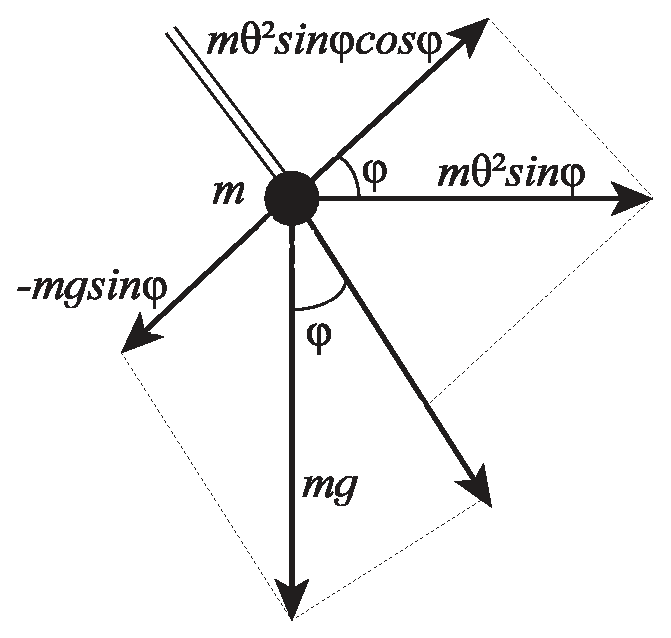
\includegraphics [scale=1]{jtr16}
	\caption{Strength and centrifugal forces.}
	\label{fig:1.6}
\end{figure}

It turns out that this system has exactly one (physically achievable) equilibrium position $(x_{0},y_{0},z_{0})$ given by equations
\begin{equation}
\label{1.12}
\cos x_{0}=F/k,\text{ \ }y_{0}=0,\text{ \ }n^{2}z_{0}^{2}=g/\cos x_{0}.
\end{equation}
In addition, the linearization matrix of the system \eqref{1.11} at this point of equilibrium is the following
\begin{equation}
\label{1.13}
A=
\begin{pmatrix}
0 & 1 & 0 \\
-g\frac{\sin ^{2}x_{0}}{\cos x_{0}} & -\frac{b}{m} & 2g\frac{\sin x_{0}}{%
	z_{0}} \\
-\frac{k}{J}\sin x_{0} & 0 & 0%
\end{pmatrix}
\end{equation}
and its characteristic polynomial is
\begin{equation}
\label{1.14}
\det \left( A-\lambda \right) =-P(\lambda )=-\left\{ \lambda ^{3}+\frac{b}{m}%
\lambda ^{2}+g\frac{\sin ^{2}x_{0}}{\cos x_{0}}\lambda +2kg\frac{\sin
	^{2}x_{0}}{Jz_{0}}\right\} .
\end{equation}

We can see that the coefficients of the polynomial $P(\lambda )$ are positive, that is, the condition (i) of the Routh-Hurwitz theorem. By Example \ref{example:1.14} (for $n = 3$) the condition for sufficient stability of the polynomial $P(\lambda )$ is the inequality \eqref{1.8}, which in this case means
\begin{equation}
\label{1.15}
\frac{bJ}{m}>2k\frac{\cos x_{0}}{z_{0}}=\frac{2F}{z_{0}}
\end{equation}
(Task 1.28). Here $\nu :=z_{0}/2F=\omega _{0}/2F$ has the mechanical interpretation of the \emph{machine unevenness}. So the last inequality is a simple one
$$
\frac{bJ\nu }{m}>1.
$$

The following conclusions can be drawn:
\begin{itemize}
	\item increasing the mass $m$ of the balls aggravates the stability;
	\item decreasing the friction coefficient $b$ aggravates the stability;\footnote{When I presented this example a few years ago at a lecture of Qualitative Theory of ODEs, Z. Nowak informed us about cases where in some German factories (where everything was taken care of) a persistent decrease in the friction coefficient led to the failure of steam engines.}
	\item reducing the moment of inertia $J$ of the flywheel aggravates the stability;
	\item a similar effect is the reduction of the machine's unevenness factor $\nu$.
\end{itemize}	
\end{example}

\section{Hyperbolicity}

The results of the previous chapter have taught us that the condition $\Re \lambda_j = 0$, for a certain value of its own linearization matrix $A$ at the point of equilibrium of the autonomous vector field
\begin{equation}
\label{1.16}
\dot{z}=Az+\ldots ,\text{ \ }z\in \left( \mathbb{R}^{n},0\right) ,
\end{equation}
is a limiting condition for solving asymptotic stability problems of this equilibrium point.
This occurs as follows

\begin{definition}
	An equilibrium point $z = 0$ of the autonomous vector field \eqref{1.16} is called \textbf{hyperbolic point}, if the real parts of all the eigenvalues of its linearization matrix $A$ of the field at this point are non-zero.
\end{definition}

Let us assume that the point $z = 0$ is hyperbolic and consider the corresponding linear system
\begin{equation}
\label{1.17}
\dot{z}=Az.
\end{equation}
Then there is a natural decomposition of the space $\mathbb{R}^n$ on the direct sum of the stable subspace $E^s \simeq \mathbb{R}^k$ and the unstable subspace $E^u \simeq \mathbb{R}^l$, corresponding to the values of $\Re \lambda_j <0$ and $\Re \lambda_j> 0$ respectively:
\begin{equation}
\label{1.18}
\mathbb{R}^{n}=E^{s}\oplus E^{u},\text{ \ \ }A=A_{1}\oplus A_{2}.
\end{equation}
Let us notice that the subspaces of $E^s$ and $E^u$ can be defined topologically in terms of the linear phase flow $g_{Az}^{t}=e^{At}$ of the linear field \eqref{1.17} (see Appendix). Namely,
$$
E^{s}=\left\{ z:g_{Az}^{t}(z)\rightarrow 0,\text{ }t\rightarrow +\infty
\right\} ,\text{ \ }E^{s}=\left\{ z:g_{Az}^{t}(z)\rightarrow 0,\text{ }%
t\rightarrow -\infty \right\}
$$
(see Figure \ref{fig:17}).

\begin{figure}[!ht]
	%\vspace{-15pt}
	\centering
	\includegraphics [scale=1.4]{jtr17}
	\caption{Hyperbolic saddle.}
	\label{fig:17}
	%\vspace{-10pt}
\end{figure}

It turns out that the analogous situation occurs in the case of the nonlinear field \eqref{1.16}.

\begin{theorem}\emph{(Hadamard-Perron).}\label{theo:1.18}
	For the hyperbolic equilibrium point $z = 0$ of the field $\dot{z} = v (z)$ of class $C^r$, $r> 2$, there exist local submanifolds, stable $W^s$ and unstable $W^u$ of class $C^r$, such that
	\begin{equation}
	\label{1.19}
	W^{s}=\left\{ z:g_{v}^{t}(z)\rightarrow 0,\text{ }t\rightarrow +\infty
	\right\} ,\text{ \ }W^{s}=\left\{ z:g_{v}^{t}(z)\rightarrow 0,\text{ }%
	t\rightarrow -\infty \right\} ,
	\end{equation}
	and\footnote{Here $g_v^t$ denotes the local phase flow generated by the field $v (x)$ and $T_y M$ denotes the tangent space to the manifold $M$ at the point $y$.}
	\begin{equation}
	\label{1.20}
	T_{0}W^{s}=E^{s},\text{ \ \ }T_{0}W^{u}=E^{u}.
	\end{equation}
\end{theorem}
Before we take the proof of this theorem, let us note that analogous concepts and theorems can be introduced for local diffeomorphisms. First, if $z = 0$ is the equilibrium point of the vector field $\dot{z}=v(z)=Az+\ldots$, then $z = 0$ is a \textbf{fixed point} of the flow transformation at time $t = 1$, $f (z) = g^1_v (z)$, i.e.,
$$
f(0)=0.
$$
In addition, the linear part $\frac{\partial f}{\partial z}(z)$ of the transformation $f$ in $z = 0$ has the form of the matrix
$$
\frac{\partial f}{\partial z}(0)=B=e^{A}.
$$
(Task 1.36). In fact, there is a discrete version of the concept of the phase portraits.

\begin{definition}
	The diffeomorphism $f:M\longmapsto M$ defines the homomorphism $\mathbb{Z}\rightarrow \textrm{Diff}(M)$ from the additive group of integers to the group of diffeomorphisms of the manifold so that
	$$
	n\longmapsto f^{n},
	$$
	where $f^{n}=f\circ \ldots \circ f$ ($n$ times for $n \geq 0$) and $f^{-n}=f^{-1}\circ \ldots \circ f^{-1}$ ($\left\vert n\right\vert $ times for $n <0$). In literature $\{f^n\}$ is called \textbf{cascade}.
	
	The point $z_0 \in M$ is a \textbf{periodic point with period} $p \geq 1$ for $f$ if $f^p (z_0) = z_0$; under this we will understand the minimum period (i.e., $f^q (z_0) \neq  z_0$ for $1 \leq q <p$).
	Of course, the periodic point with period $p = 1$ is a fixed point.
\end{definition}

\begin{definition}
	The periodic point $z_0$ of period $p$ of the diffeomorphism $f$ is called \textbf{hyperbolic} if the matrix
	$$
	B=\frac{\partial (f^{p})}{\partial z}(z_{0})
	$$
	has all its eigenvalues outside of a unitary range,
	$$
	\left\vert \lambda _{j}\right\vert \not=1.
	$$
\end{definition}

\begin{lemma}\label{lemma:1.21}
	If $z = 0$ is a hyperbolic equilibrium point for the vector field $v (z)$, then $z = 0$ is also a hyperbolic fixed point of the diffeomorphism $f = g^t_v$, and vice versa \emph{(Task 1.36)}.
\end{lemma}

We have the following version of the Hadamard-Perron theorem for diffeomorphisms.

\begin{theorem}\label{theo:1.22}
	If the fixed point $z=0$ of the local diffeomorphism $f:\left( \mathbb{R}^{n},0\right) \longmapsto
	\left( \mathbb{R}^{n},0\right) $ of class $C^r$, $r \geq 1$, is hyperbolic, there are local subspaces, stable $W^s$ and unstable $W^u$ of class $C^r$, such that
	\begin{equation}
	\label{1.21}
	W^{s}=\left\{ z:f^{n}(z)\rightarrow 0,\text{ }n\rightarrow +\infty \right\} ,%
	\text{ \ }W^{s}=\left\{ z:f^{n}(z)\rightarrow 0,\text{ }n\rightarrow -\infty
	\right\} ,
	\end{equation}
	and
	\begin{equation}
	\label{1.22}
	T_{0}W^{s}=E^{s},\text{ \ \ }T_{0}W^{u}=E^{u},
	\end{equation}
	where $E^s$ and $E^u$ are subspaces of $\mathbb{R}^n$ extracted by their own subspaces corresponding to the eigenvalues of the matrix $B=\frac{\partial f}{\partial z}(0)$ of module $< 1$ and $> 1$ respectively.
\end{theorem}

The path to the proof of the Hadamard-Perron Theorem \ref{theo:1.18} goes through the proof of Theorem \ref{1.22}. 
At the same time, as we shall soon see, the method of proof of the existence of submanifolds $W^s$ and $W^u$ with properties \eqref{1.21} of class $C^0$ is quite natural:
one gets the equation into a fixed point of some transformation in the appropriate infinitely dimensional Banach space.
Unfortunately, `squeezing' the condition of contraction of this transformation is very exhausting.
Therefore, in the following proof we will limit ourselves to deriving the appropriate equations and sketch a general estimation scheme.
For strict proof, we refer the reader to the monograph of W. Szlenk \cite{Szl}.

\begin{proof}[Proof of Theorem \ref{theo:1.22}]
	To simplify the situation, let's assume the decomposition \eqref{1.18}, that is, $\mathbb{R}^{n}=E^{s}\oplus
	E^{u}=\left\{ \left( x,y\right) \right\} $ and the transformation into the form $f=\left( f_{1},f_{2}\right) $, such that
	\begin{equation}
	\label{1.23}
	f_{1}(x,y)=Ax+\varphi (x,y),\text{ \ \ }f_{2}(x,y)=By+\psi (x,y),
	\end{equation}
	where
	\begin{equation}
	\label{1.24}
	\left\Vert A\right\Vert <1,\text{ \ \ \ }\left\Vert B^{-1}\right\Vert <1
	\end{equation}
	and the functions $\varphi $ and $\psi $ are ordered in $O(\left\vert
	x\right\vert +\left\vert y\right\vert )$ (Task 1.37).
	
	Of course, the vector functions $\varphi $ and $\psi $ are defined in a small neighborhood of zero. In the proof, which is presented below, this is a technical obstacle. Therefore, we will make the following change $$
	\varphi \longmapsto \varphi \chi ,\text{ \ \ }\psi \longmapsto \psi \chi ,
	$$ where function $\chi (x,y)$ is smooth (class $C^{\infty }$) and such that:
	\begin{enumerate}[(i)]
		\item $\chi (x,y)\geq 1$ in a small neighborhood of zero, $\left\vert
		x\right\vert +\left\vert y\right\vert <\varepsilon $;
		\item $\chi (x,y)\equiv 0$ outside the small neighborhood of zero, $\left\vert
		x\right\vert +\left\vert y\right\vert >2\varepsilon $ (Task 1.38).
	\end{enumerate}
	Thus, the functions $\varphi \chi $ and $\psi \chi $ after the zero extension for $\left\vert x\right\vert +\left\vert y\right\vert >\varepsilon $ will be determined around $\mathbb{R}^{n}$. Next we mark them with $\varphi $ and $\psi $. Recall that these new functions satisfy $d\varphi (0,0)=0$, $d\psi (0,0)=0$, and $\left\vert \varphi \right\vert $ and $\left\vert \psi \right\vert $ are small with derivatives. By the property (i) the dynamics of the transformation $f$ with the new $\varphi $ and $\psi $ in the zero neighborhood is the same as for the old transformation \eqref{1.23}.
	
	We are looking for a variation of $W^s$ in the form of a graph of a certain mapping (or vector function) $F:E^{s}\longmapsto E^{u}$,
	$$
	W^{s}=\left\{ (x,F(x)):x\in E^{s}\right\} .
	$$
	(Proof of the existence of the $W^{u}$ submanifold is quite similar, so we are confined to the case of $W^{s}$.)
	
	From property \eqref{1.21} it follows that the $W^{s}$ submanifold should be invariant over the diffeomorphism $f,$ $f(W^{s})=W^{s}.$ This means that $f(x,F(x))=(x_{1},F(x_{1}))$ for some $x_{1}\in E^{s}$ depending on $x\in E^{s}$. From \eqref{1.23} we find that $x_{1}=Ax+\varphi (x,F(x)).$ So we get the condition
	$$
	BF(x)+\psi (x,F(x))=F\circ (Ax+\varphi (x,F(x)),
	$$
	that we will write in the following form
	\begin{equation}
	\label{1.25}
	F(x)=B^{-1}\left\{ F\circ (Ax+\varphi (x,F(x))-\psi (x,F(x))\right\} =:%
	\mathcal{T}(F)(x).
	\end{equation}
	We treat the last equation as a fixed point equation $F=%
	\mathcal{T}(F)$ for a nonlinear operator $\mathcal{T}$ defined by the right side of this equality.
	
	Assuming that the functions $ \varphi $ and $ \psi $ are of class $ C^{1} $, it is natural to introduce the Banach space $ \mathcal {X}%
	= C ^ {0} (E ^ {s}, E ^ {u}) $ continuous mapping with supremum norm. It is easy to show that the transformation $ \mathcal {T} $ carries $ \mathcal {X} $ in itself. In order to apply the Banach theorem for constraint mappings, it is still necessary to prove the contradiction condition, they estimate the norm of the difference $ \mathcal {T} (F_ {1}) - \mathcal {T} (F_ {2})$. Here comes the problem, because of (1.25) we get the following inequality:
	$$
	\left\Vert \mathcal{T}(F_{1})-\mathcal{T}(F_{2})\right\Vert
	\leq \left\{ \left\Vert B^{-1}\right\Vert +\left\Vert B^{-1}\right\Vert
	\cdot \left\Vert F_{1}^{\prime }\right\Vert \cdot \left\Vert \varphi
	_{y}^{\prime }\right\Vert +\left\Vert B^{-1}\right\Vert \cdot \left\Vert
	\psi _{y}^{\prime }\right\Vert \right\} \cdot \left\Vert
	F_{1}-F_{2}\right\Vert
	$$
	(Task 1.39). Since $ \left \Vert B ^ {- 1} \right \Vert <1 $ \ (see \eqref{1.24}) and $\left\Vert \psi _{y}^{\prime }\right\Vert =\left\Vert \partial
	\psi /\partial y\right\Vert $ and $\left\Vert \partial \varphi /\partial
	y\right\Vert $ are small (see above), it is only possible to estimate the norm of the derivative $ F_ {1} ^ {\prime} $ mapping $ F_ {1}$. But if we choose $ F_ {1} $ and $ F_ {2} $ arbitrarily from space $ \mathcal {X}$, then  $ F_ {1} $ will only be continuous, and its derivative can be unlimited.
	
	It is out of this deadlock. Let us recall that in the proof of Banach's theorem we choose $ F_ {0} \in \mathcal {X}$, then $ f_ {n} = \mathcal {T} ^ {n} (F_ {0}) $ should converge to a fixed point. The point is to choose the vector function $ F_ {0} $ to show that the functions $ F_ {n} $ are also smooth with appropriately limited norms. It is easy to guess that
	$$
	F_{0}(x)\equiv 0
	$$
	is a good choice. It is also easy to see from formula \eqref{1.24} that $ F_ {n} (x) $  are smooth, e.g. $F_{1}(x)=-B^{-1}\psi (x,0).$
	
	You just have to show that the functions $ F_ {n} (x) $ are uniformly constant. This is reduced to estimate the derivative norm$\left( \mathcal{%
	T(}F)\right) ^{\prime }(x)$ on the assumption, the limits of the norm $ F ^ {\prime} (x)$. We have 
	\begin{equation}
	\label{1.26}
	\left( \mathcal{T(}F)\right) ^{\prime }(x)=B^{-1}\cdot \left\{ F^{\prime
	}\cdot \left[ A+\varphi _{x}^{\prime }+\varphi _{y}^{\prime }\cdot F^{\prime
	}\right] -\psi _{x}^{\prime }-\psi _{y}^{\prime }\cdot F^{\prime }\right\} ,
	\end{equation}
	where we omitted the arguments of the functions appearing on the right side of this equality. Thus the supremum standard is estimated as follows:
	$$
	\left\Vert \left( \mathcal{T(}F)\right) ^{\prime }\right\Vert \leq
	a+b\left\Vert F^{\prime }\right\Vert +c\left\Vert F^{\prime }\right\Vert
	^{2},
	$$
	where $ a $ is small, $ b <1 $ and $ c> 0. $ Hence, if $\left\Vert F^{\prime }\right\Vert $ is small enough, $\left\Vert
	F^{\prime }\right\Vert <d$ (for the appropriate $ d $), then $\left\Vert \left(\mathcal{T(}F)\right) ^{\prime }\right\Vert <d$ (Task 1.40). This gives an even estimate for the norm $ \left \Vert F_ {n} ^ {\prime} \right \Vert $ of the function $ F_ {n}. $
	
	So $ F_ {n} $ converges to the fixed point $ F _ {\ast}$, which we can only say for the time being that it is represented by a continuous mapping of $ E ^ {s} $ to $ E ^ {u } $; that is the submanifold
	$$
	W^{s}=\left\{ (x,F_{\ast }(x))\right\}
	$$
	is of class $ C ^ {0}. $
	
	Let us briefly explain how to measure the smoothness of the function $ F _ {\ast}$. To do this, the equations \eqref{1.25} and \eqref{1.26} must be applied simultaneously to the strings $ \left \{F_ {n} \right \} $ and $\left \{F_ {n} ^ {\prime} \right \} $. In particular, the continuity of the family $ \left \{F_ {n} ^ {\prime} \right \}$, which requires a uniform estimation of the expression
	$\sup \left\vert \left( \mathcal{T(}	F_{n})\right) ^{\prime }(x_{1})-\left( \mathcal{T(}F_{n})\right) ^{\prime}(x_{2})\right\vert $. It turns out that this can be done using the estimates for 
	$\sup \{\left\vert
	F_{n}^{\prime }(x_{1})-F_{n}^{\prime }(x_{2})\right\vert $, $\left\vert
	\varphi ^{\prime }(x_{1},y_{1})-\varphi ^{\prime }(x_{2},y_{2})\right\vert $, $\left\vert \psi ^{\prime }(x_{1},y_{1})-\psi ^{\prime
	}(x_{2},y_{2})\right\vert \}$.

	Then, Ascoli's theorem is used, which says that from a uniformly continuous function on a compact set, one can choose a convergence. Here the compact set is $\left\{ \left\vert x\right\vert <M\right\} \subset E^{s}$ for some $ M $ and the boundary of $ \left \{F_ {n_ {k}} \right \} $ must be $ F _ {\ast} $ (because there is a boundary in the continuous function space).
		
	In this (shortened) proof we limit ourselves to the case where $ f $ is of class $ C ^ {1} $ (and then $ W ^ {s, u} $ are also classes $ C ^ {1}) $. But the case of the class $ C ^ {r} $ for $ r> 1 $ can also be proved by the same method, only the proof requires a larger number of formulas and estimates. We skip it.
	
	Finally, let us note that since $ F_ {0} ^ {\prime} (0) = 0 $ and $ \varphi ^ {\prime} (0,0) = 0 $ and $\psi ^{\prime }(0,0)=0,$ then we have $ F_ {\ast} ^ {\prime} (0) = 0, $ which means that the submanifold $ W ^ {s} $ is tangent to $ \left (0,0 \right) $ to the space $ E ^ {s} $.
\end{proof}

\begin{proof}[Proof of Theorem \ref{theo:1.18}]
	Let us assume $ f = g_ {v} ^ {1}$, that is, transforming the phase flow after time $ t = 1 $ and let $ V ^ {s} $ be a local stable manifold for $ f $ (see Theorem \ref{theo:1.22}). Since the submanifold $ W ^ {s} $ is defined topologically as a set of these points $ z $, that $ g_ {v} ^ {t} (z) \rightarrow 0 $  when $ t \rightarrow \infty$, then $ W ^ {s} \subset V ^ {s} $. On the other hand, if $ z \in V ^ {s} $, then writing $ t = n + \tau $ for $ n \in \mathbb {N} $ and $ 0 \leq \tau <1$, we have $g^{t}(z)=g^{\tau
	}(g^{n}(z))\rightarrow 0$ (as the family $\left\{ g^{\tau }\right\}_{\tau \in \lbrack 0,1)}$ is uniformly continuous).
\end{proof}

The second basic result for hyperbolic fixed points is from D. Grobman and P. Hartman (\cite {Hart}). We formulate it simultaneously for cascades and streams.

\begin{theorem}\emph{(Hartman-Grobman).}\label{theo:1.23}
	Let $f:\left( \mathbb{R}^{n},0\right) \longmapsto \left( \mathbb{R}^{n},0\right) $ be a diffeomorphism of class $C^1$, $r\geq 1$, with a hyperbolic fixed point at $z=0$. Then there is a local homeomorphism $ h: \left (\mathbb {R} ^ {n}, 0 \right) \longmapsto \left( \mathbb{R}^{n},0\right) $ so that
	\begin{equation}
	\label{1.27}
	h\circ f'(0)=f\circ h(z).
	\end{equation}
	
	Analogously, for a local flow $ g_ {v} ^ {t} $ generated by the germ of the vector field $ v \left (z \right)$ with the hyperbolic equilibrium point $ z = 0 $, there is a local homeomorphism $ h $ (as above) that
	\begin{equation}
	\label{1.28}
	h\circ e^{tv^{\prime }(0)}(z)=g_{v}^{t}\circ h(z).
	\end{equation}
	
	\begin{proof}
		Let's start with the cascade case. Similarly to the proof of Theorem \ref{theo:1.22}, we introduce the situation to the case where $ z = \left (x, y \right) $ and
		$$
		f(x,y)=(Ax+\varphi ,By+\psi )=Lz+\tilde{f},
		$$
		where $L=A\oplus B=f^{\prime }(0)$ estimates \eqref{1.24} and $\tilde{f}=\left( \varphi (x,y),\psi (x,y)\right) $ is defined as the whole $ \mathbb {R} ^ {n} = E ^ {s} \oplus E ^ {u} $ and is small with derivatives. Homeomorphism $ h $ will be chosen in the form
		\begin{equation}
		\label{1.29}
		h=id+g=(x+g_{1},y+g_{2}),\text{ \ \ }g\text{\ small.}
		\end{equation}
		
		Equation \eqref{1.27} on $ h $, which denotes the alternation of the following diagram
		$$
		\begin{array}{ccc}
		\mathbb{R}^{n} & \overset{f}{\longmapsto } & \mathbb{R}^{n} \\
		\uparrow h &  & \uparrow h \\
		\mathbb{R}^{n} & \overset{L}{\longmapsto } & \mathbb{R}^{n}%
		\end{array}%
		$$
		leads to equation $\left( id+g\right) \circ L=L (id+g)+\tilde{f} \circ (id+g)$. In the composition we get the system of equations
		$$
		\begin{array}{lll}
		g_{1}(Ax,By) & = & A g_{1}(x,y)+\varphi (x+g_{1},y+g_{2}), \\
		g_{2}(Ax,By) & = & B g_{2}(x,y)+\psi (x+g_{1},y+g_{2}).
		\end{array}
		$$
		Let's rewrite this layout in a convenient way for us
		\begin{equation}
		\label{1.30}
		\begin{array}{lll}
		g_{1}(x,y) & = & A g_{1}(A^{-1}x,B^{-1}y)+\varphi \circ (id+g)\circ
		(A^{-1}x,B^{-1}y), \\
		g_{2}(x,y) & = & B^{-1} g_{2}(Ax,By)-B^{-1}\cdot \psi \circ (id+g).%
		\end{array}
		\end{equation}
		It is easy to recognize here the equation of the fixed point $ g = \mathcal {T} (g) $ for the nonlinear operator $ \mathcal {T} $ acting on $ g = (g_ {1}, g_ {2}) $ by the right hand side of \eqref{1.30}.
		
		We will choose the Banach space
		$$
		\mathcal{X}=C^{0}(\mathbb{R}^{n},E^{s})\oplus C^{0}(\mathbb{R}^{n},E^{u})
		$$
		with norm $\left\Vert g\right\Vert =\sup \left\vert g_{1}\right\vert +\sup
		\left\vert g_{2}\right\vert $. Here it is easy to show that the operator $ \mathcal {T} $ converts a sphere in $ \mathcal {X} $ with a proper radius in itself and is a contraction. The basic argument is that $ A $ and $ B ^ {- 1} $ matrices have a norm $ <1 $.
		
		Let us break away for a moment from our proof and consider the situation when equation \eqref{1.27} is replaced by equation
		\begin{equation}
		\label{1.31}
		k\circ f=L\circ k,
		\end{equation}
		where $k:\mathbb{R}^{n}\longmapsto \mathbb{R}^{n}$. After the substitution $k=id+l=(x+l_{1},y+l_{2})$ and some transformations, we get the following system analogue to \eqref{1.30}:
		$$
		\begin{array}{lll}
		l_{1}(x,y) & = & Al_{1}\circ f^{-1}(x,y)-\varphi \circ f^{-1}(x,y), \\
		l_{2}(x,y) & = & B^{-1}l_{2}(x,y)+B^{-1}\psi (x,y).%
		\end{array}%
		$$
		Here we are dealing with a fixed point equation for the corresponding transformation of $ \mathcal {S}: \mathcal {X} \longmapsto \mathcal {X} $, which is coherent. So also the system \eqref{1.31} has a solution.
		
		Let us note the following property of solutions of equations \eqref{1.27} and \eqref{1.31}, which are the consequence of the fact that in Banach's thesis the fixed point of convergence in the Banach space is constant depending on the parameters (if the transformation itself depends on the parameters continuously):
		
		\emph{The solutions $ h (x, y) $ and $ k (x, y) $ of the equations \eqref{1.27} and \eqref{1.31} are unique and depend in a continuous manner on the data in these equations (i.e. $ L = A \oplus B $ and $ \tilde {f} = (\varphi, \psi)) $. In addition, in equation \eqref{1.27} we can substitute the linear transformation $ L = f ^ {\prime} (0) $ by any transformation $ g $ such that $ g ^ {\prime} (0) = L$.}
		
		The above-mentioned uniqueness will allow us to prove that the transformations $ h $ and $ k $ are homeomorphisms; more precisely, $ h \circ k = k \circ h = id $. In fact, the transformation $ m = k \circ h $ satisfies the condition $ m \circ L = L \circ m$, at equation \eqref{1.27} for $ f = L $. Analogously, the transformations $ n = h \circ k $ and $ id $ satisfies the equation $ f \circ n = n \circ f $.
		
		Let's now take a proof of the second part of the theorem, that is, the homeomorphism of $ h $, which satisfies all of the equations of type \eqref{1.27} for the family of transformations $ f_ {t} = g_ {v} ^ {t}, $ $ v = Az + \ldots $. For each $ t \not = 0 $  the transformation $ f_ {t} $  have the hyperbolic fixed point $ z = 0 $. Thus, from the proved part of the first part of the theorem we have the existence of a family of homeomorphisms $ h_ {t} $, $ t \not = 0 $, such that
		$$
		h_{t}\circ e^{At}=f_{t}\circ h_{t}.
		$$
		We just have to show that $ h_ {t} $ does not depend on $ t $, which we treat here as a parameter. At least we know that $ h_ {t} $ depends on $ t $ in a continuous manner.
		
		Let us now define the following identity
		$$
		h_{t/2}\circ f_{t}\circ h_{t/2}^{-1}=\left( h_{t/2}\circ f_{t/2}\circ
		h_{t/2}^{-1}\right) \circ \left( h_{t/2}\circ f_{t/2}\circ
		h_{t/2}^{-1}\right) =e^{At/2}\circ e^{At/2}=e^{At}
		$$
		(here we used the group property of the phase flow). It means that $ h_ {t / 2} = h_ {t} $ (uniqueness). Similarly it is proved that $ h_ {t / k} = h_ {t} $  for natural $ k $  and hence that
		$$
		h_{kt/l}=h_{t},\text{ \ \ }k,l\in \mathbb{N},
		$$
		(Task 1.41). Let us say that for a measurable set of parameters $ t $ the transformations $ h_ {t} $ are the same. The constant $ h_ {t} $ of the parameter (see above) implies $ h_ {t} \equiv \textrm {const} $ as a function from $ t> 0 $. Now observe that if $ h $ satisfies the equation \eqref{1.28} for a given time $ t> 0$, then this equation for $ -t $ (Task 1.42) ends the proof.
		
		Finally, one more note.	Since $ \left \{g_ {v} ^ {t} \right \} $ is only a local phase potentiometer (for the vector field $ v (z)$ defined in the neighborhood of $ z = 0$) it is necessary to take care of the fields of the transformations of the flow, and thus to the domains of transformations $ h_ {t} $. But there is no problem here because the domain of transformation $ g_ {v} ^ {t / k} $ increases with the increase of $ k \in \mathbb {N} $. Just in the above proof, we limit ourselves to times such that $ \left \vert t \right \vert <1 $.
	\end{proof}
\end{theorem}

Equality \eqref{1.27} means that the dynamics (i.e. cascade) generated by the diffeomorphism $ f $  is the same from the qualitative point of view as the dynamics generated by the linear diffeomorphism $L (z) = f ^ {\prime}(0)z $. Indeed, if $\left\{ \ldots, f^{-1}(z_{0}), z_{0}, f(z_{0}), f^{2}(z_{0}), \ldots \right\} $ is the orbit of the point relative to the diffeomorphism $ f $ and $y_{0}=h(x_{0})$, then $\{\ldots, L^{-1}(y_{0}), y_{0},\linebreak L(y_{0}), \ldots \}$ is the orbit of the point $y_{0}$ relative to the linear diffeomorphism $ L $.

The following definition seems natural.

\begin{definition}\label{def:1.24}
	If for the diffeomorphisms $ f: M \longmapsto M $ and $ g: N \longmapsto N $  there exists a homeomorphism $ h: M \longmapsto N $  such that
	$$
	g=h\circ f\circ h^{-1},
	$$
	we say that the diffeomorphism $ f $ and $ g $ are \textbf {topologically conjugated} (via $ h $). If $ h $ is of class $ C ^ {r} $, then we say that $f$ and $g$ are \textbf{$ C ^ {r} $-conjugated}. Similarly, the vector fields $ v (x) $ and $ w (x) $ are topologically (or classes $ C ^ {r}) $  \textbf{conjugated} if their phase flows are conjugated by a homeomorphism (or diffeomorphism of class $ C ^ {r}) $.
	
	If the diffeomorphism $ f $ has the property that any diffeomorphism $ g $ which is close to $ f $ (in a class that we do not want to emphasize here) is topologically conjugated with $ f $, then we say that $ f $ is \textbf {structurally stable}. Similarly, the vector field $ v (x) $ is \textbf {structurally stable} if the close vector fields are topologically conjugated to it.
\end{definition}

Hartman-Grobman's theorem states that the diffeomorphism (vector field, respectively) in the hyperbolic fixed point (hyperbolic equilibrium point, respectively) is topologically conjugated to the linear part of the diffeomorphism (vector field, respectively). We can prove more.

\begin{proposition}\label{prop:1.25}
	A diffeomorphism (vector field, respectively) in a neighborhood of a hyperbolic fixed point (hyperbolic equilibrium, respectively) is structurally stable.
	\begin{proof}
		We use the following direct construct of the homeomorphism $ h $, which associates two divergent diffeomorphisms $ f $ and $ g $ in the case of the asymptotically stable, i.e., that $ f ^ {\prime} (0) $ and $ g ^ {\prime} (0) $ have all their own values of module $ <1 $. It can be assumed that $ E ^ {s} = \mathbb {R} ^ {n} $ and $ z = x $ in the proof of Hartman-Grobman theorem. Then there is a `Lyapunov function', $ L (x) $, such that satisfies condition (i) of Definition \ref{def:Lyap_funct} and the following analogous condition to (ii):
		$$
		L(f(x))<L(x)\text{ \ for \ }x\not=0.
		$$
		Its construction is exactly the same as in the proof of the Lyapunov Theorem. We can assume that $ L (x) = \left \vert x \right \vert ^ {2} $ in the corresponding (linear) coordinate system. Let $ M (x) = \left \vert x \right \vert ^ {2} $ be the corresponding Lyapunov function for the $ g $ diffeomorphism (also in the corresponding coordinate system). We have two copies of $ \mathbb {R} ^ {n} $, which deal respectively with the diffeomorphisms $ f $ and $ g $.
		
		\begin{figure}[!ht]
			%\vspace{-15pt}
			\centering
			\includegraphics [scale=1.1]{jtr18}
			\caption{Coupling construction.}
			\label{fig:1.8}
			%\vspace{-10pt}
		\end{figure}	
	Let us take a small $ \varepsilon> 0 $ and consider hyperplanes (diffeomorphic with spheres) $ \left \{L (x) = \varepsilon \right \} $ i $ \left \{M (x) = \varepsilon \right \} $. Let's define the homeomorphism $ h $ between these hyperplanes as $ h|_{L = \varepsilon} = id: \left \{L = \varepsilon \right \} \longmapsto \left \{M = \varepsilon \right \} $ (see Figure \ref{fig:1.8}). Condition 
	\begin{equation}
	\label{1.32}
	h\circ f^{-1}=g^{-1}\circ h
	\end{equation}
	allows us to `transform' $ h $ between the hyperplanes $f(\left\{ L=\varepsilon \right\} )$ and $g\left( \left\{ M=\varepsilon \right\} \right)$, as shown in Figure \ref{fig:1.8}. Let $ h $ be continuous and mutually exclusive to the area between hyperplanes $ \left \{L = \varepsilon \right \} $ and $ f \left (\left \{L = \varepsilon \right \} \right ) $. Using the multiple equation \eqref{1.32} extends us $ h $ to the whole area $ \left \{0 <L \leq \varepsilon \right \} $. By putting $ h (0) = 0 $ we get the desired homeomorphism.
	
	The analogous construction works in the case of extending diffeomorphisms, i.e., when the $ f ^ {\prime} (0) $ and $ g ^ {\prime} (0) $ have their eigenvalues with module $> 1 $.
	
	Let's now consider two linear diffeomorphisms $ f_ {0} $ and $ g_ {0} $ defined by the hyperbolic matrix $ A = A_ {s} \oplus A_ {u} $ and $ B = B_ {s} \oplus B_ {u}$ in the corresponding (and the same) distributions $ \mathbb {R} ^ {n} = E ^ {s} \oplus E ^ {u} $. From the above considerations, we get the homeomorphisms $ h_ {s} $ and $ h_ {u} $, which join $ A_ {s} x $  with $ B_ {s} x $  and $ A_ {u} y $ with  $ B_ {u} y $ respectively. Now, the homeomorphism 
	$$
	h=h_{s}\oplus h_{u}
	$$
	takes $ f_ {0} $ to $ g_ {0}$.
	
	Let's now consider the $ f $ diffeomorphism in the neighborhood of the hyperbolic fixed point $ z = 0 $ and its small disturbance $ g $ with the same fixed point. Since the matrix $B=g^{\prime }(0)$ is close to the matrix $ A = f ^ {\prime} (0) $ is also hyperbolic with the same dimensions of the stable and unstable subspaces; that is, we can apply the above construction of the homomorphic homeomorphism of the linear parts of these diffeomorphisms. We see that $ f $ is conjugated with $ f_ {0} = f ^ {\prime} (0)z $, $ f_ {0} $ is conjugated with $ g_ {0} = g ^ { \prime} (0) z $ and $ g_ {0} $ is conjugated with $ g $; by comparing these three homeomorphisms one gets that $ f $ is conjugated with $ g $.
	
	The case of Proposition \ref{prop:1.25} for vector fields is left to the readers as an exercise (Task 1.43).
	\end{proof}
\end{proposition}

\begin{remark}
	You can ask if Grobman-Hartman's thesis can be strengthened, i.e., if the homeomorphism $ h $ can be of class $ C ^ {1} $. It turns out that no. For example, the transformation $ \left (x, y, z \right) \longmapsto \left (\frac {1} {2} x, 4y, 2z + xy \right) $ can not be linearized using a  $C ^ {1} $-diffeomorphism   (see \cite {Hart}, Problem 8.1). This problem is related to resonances between eigenvalues (see Poincaré Theorem in Chapter \ref{sec:3.3}).
\end{remark}

\subsection*{Tasks}
\begin{task}
	Complete the proof of Lemma \ref{lemma:1.7}, i.e., in case of non-real values.
\end{task}
\begin{task}
	Prove the formulas $(1.11)$ - $(1.15)$.
\end{task}
\begin{task}
	Determine the stability (in Lyapunov and asymptotic terms) for the singular point $ x = d / c $, $ y = a / b $, at the Lotka-Volterra system
	\begin{equation}
	\label{1.33}
	\dot{x}=x(a-by),\text{ \ \ }\dot{y}=y(cx-d),\text{ \ \ }abcd>0,
	\end{equation}
	which describes the dynamics of two competing populations (predators and preys).
	
	Note: Proposition \ref{prop:2.11} below.
\end{task}
\begin{task}
	Using the Definition \ref{def:1.1}, check that the equilibrium point $ x (0) = 0 $ for the equation $ \dot {x} = 4x-t ^ {2} x $ is stable in Lyapunov's sense, i.e., with $ t_ {0} = 0 $.
\end{task}
\begin{task}
	Determine the stability of the equilibrium point $ x = y = 0 $ for the system $ \dot {x} = e ^ {x + 2y} - \cos 3x $, $ \dot {y} = \sqrt {4 + 8x} 2e^ {y} $.
\end{task}
\begin{task}
	Determine the stability of the solution of $ \dot {x} = e ^ {x} -e ^ {3z} $, $ \dot {y} = 4z-3 \sin (x + y) $,  $ \dot { z} = \ln (1 + z-3x) $.
\end{task}
\begin{task}
	For what value of $ a $, the solution of $ \dot {x} = ax + y + x ^ {2} $, $ \dot {y} = x + ay + y ^ {2} $ is asymptotically stable?
	
	Note: When $ a = -1 $, the straight $ y = x $ is invariant.
\end{task}
\begin{task}
	For what parameters of $ a $ and $ b $, the solution of $\dot{x}=y+\sin x$, $\dot{y}=ax+by$ is asymptotically stable?
	
	Note: for $ a = b \leq -1 $, by introducing $ z = \dot {x} $, the system returns into $ \dot {x} = H_ {z} ^ {\prime} $, $ \dot {z} = {H} {x} ^ {\prime} - (a + \cos x) z$, $H=\frac{1}{2}z^{2}-a(\frac{1}{2}x^{2}+1-\cos x)$, and find the Lyapunov function.
\end{task}
\begin{task}
	For what parameters of $ a $ and $ b $, the solution $ x (t) \equiv 0 $ of the equation $ \dddot {x} +3 \ddot {x} + a \dot {x} + bx = 0 $ is asymptotically stable?
\end{task}
\begin{task}
	Show that the diffeomorphism $ g ^ {t} $ (locally) of the phase flow generated by the vector field $ \dot{x}=Ax+O\left( \left\vert x\right\vert ^{2} \right)$ has a linear part at the fixed point $ x = 0 $ of the form $ B = e ^ {At} $. From here, deduce Lemma \ref{lemma:1.21}.
\end{task}
\begin{task}
	Prove the estimates \eqref{1.24} (for the corresponding coordinate system and Euclidean norm in $ \mathbb {R} ^ {n}) $.
\end{task}
\begin{task}
	Give the explicit formula to the function $ \chi $ from proof of Theorem \ref{theo:1.22}.
\end{task}
\begin{task}
	Prove the inequalities for $ \left \Vert \mathcal {T} (F_ {1}) - \mathcal {T} (F_ {2}) \right \Vert $  from proof of Theorem \ref{theo:1.22}.
\end{task}
\begin{task}
	Give a formula for $ d $, depending on $ a, b, c $, in terms of $ \left \Vert (\mathcal {T} (F)) ^ {\prime} \right \Vert <d $.
\end{task}
\begin{task}
	Prove that $h_{\frac{k}{l}t}=h_{t}$ for $ k, l \in \mathbb {N} $ and $ t \not = 0 $.
\end{task}
\begin{task}
	Prove that if $ h $ satisfies property \eqref{1.28} for a given $ t> 0 $ then it also satisfies this property for $ t <0 $.
\end{task}
\begin{task}
	Complete the proof of Proposition \ref{prop:1.25}.
\end{task}
\chapter{Phase portraits of autonomous vector fields}

\begin{definition}\label{def:2.1}
	The \textbf{phase portrait} of an autonomous vector field $ v (x) $ on a manifold $ M $ is the partition of $ M $ into the phase curves of this field.
\end{definition}

Phase curves are of three types:
\begin{enumerate}[(i)]
	\item equilibrium points, i.e., degenerated curves corresponding to fixed solutions;
	\item embedded intervals (bounded or not); i.e., the images $\varphi(I)$ of the solutions of $\varphi :I\longmapsto M$, which are embedded;
	\item \textbf{closed phase curves} (embedded circles) corresponding to \textbf{periodic solutions} $\varphi :$
	\begin{equation}
	\label{2.1}
	\varphi (t+T)=\varphi (t),\text{ \ \ }t\in \mathbb{R},
	\end{equation}
	where $ T> 0 $ is the expansion \textbf{period} (we assume that this is the minimum period satisfying \eqref{2.1}).
\end{enumerate}

Throughout this chapter we only consider autonomous vector fields; therefore, we will leave the adjective `autonomous'.

\begin{example} (Mathematical pendulum).\label{example:2.2}
	This is the following system
	$$
	\dot{x}=y,\text{ \ \ }\dot{y}=-\sin x
	$$
	over phase space $M=\mathbb{S}^{1}\times \mathbb{R}$ (cylinder).
	\begin{figure}[!ht]
		\centering
		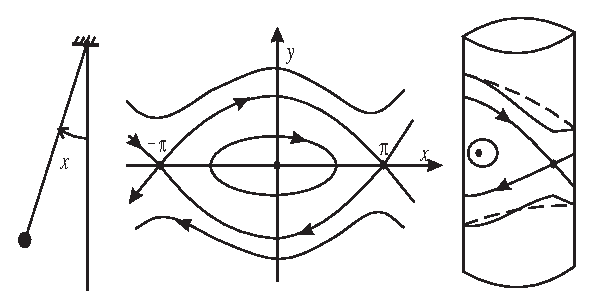
\includegraphics [scale=1.1]{jtr21}
		\caption{Pendulum.}
		\label{fig:2.1}
	\end{figure}
	
	It is easy to see that the function 
	\begin{equation}
	\label{2.2}
	H=\frac{1}{2}y^{2}-\cos x
	\end{equation}
	is the first integral of this system, i.e., $ \dot {H} \equiv 0 $. Notice the following properties of $ H: $
	\begin{itemize}
		\item point $\left( 0,0\right) $ is an absolute minimum point and $ H (0,0) = -1 $;
		\item point $\left( \pi ,0\right) $ is a saddle point and $ H (\pi, 0) = 1 $;
		\item $H(x,y)\rightarrow \infty $ as $\left\vert y\right\vert
		\rightarrow \infty $.
	\end{itemize}

It is also easy to see that, in addition to the above equilibrium points, we have two phase curves of type (ii); these are the separatrices of the saddle point $\left( \pi ,0\right) $ lying in the level $\left\{ H=1\right\}$. The remaining phase curves are closed and can be divided into two groups: (a) around the equilibrium point $(0,0)$ (corresponding to fluctuations of limited
amplitude) and (b) circulating cylinder (they correspond to the pendulum spinning around the anchor point).

We can calculate the periods of the above periodic solutions lying on the level $ H = h $ of the first integral. We have $ dt = dx / y$, where $ y $ is given by formula \eqref{2.2}: $y=\pm \sqrt{2(h+\cos x)}$. So in case (a) we have
$$
T=2\int_{x_{1}}^{x_{2}}\frac{dx}{\sqrt{2(h+\cos x)}},
$$
where $ x_ {1,2} $ are two zeros of function $ h + \cos x $. Here, from $ x_ {1} $ to $ x_ {2} $, the trajectory length is $ y> 0 $, but for symmetry it is exactly half the period. In case (b) we have
$$
T=\int_{0}^{2\pi }\frac{dx}{\sqrt{2(h+\cos x)}}.
$$

Unfortunately, the above can not be counted in terms of elementary functions. In fact, after substituting $ u = \cos x $ (with $ dx = du / \sin x = -du / \sqrt {1-u ^ {2}}) $ we get 
$$
T=4\int_{-h}^{1}\frac{du}{\sqrt{(1-u^{2})(h+u)}}.
$$
The right side of the last equation is the called \textit {elliptic integral} defining a certain elliptic function\footnote{Ellipses and elliptic functions appear very often in differential equations of classical mechanics (see \cite{Ar3}).} (Task 2.45).

We also notice that the closed phase curves in this example are not isolated, they are in whole families.
\end{example}

\section{Periodic solutions}

Closed phase curves are also called periodic trajectories or periodic orbits. In Example \ref{example:2.2}, they exist in whole families, but there are also periodic trajectories isolated.

\begin{definition}
	An isolated closed phase curve of an autonomous vector field is called  \textbf{limit cycle}.
	
	The equilibrium point of such a field, which is surrounded by non-isolated closed phase curves, is called \textbf {center}.
\end{definition}

\begin{example}\label{example:2.4}
	Let's consider the system
	$$
	\dot{x}=x(1-x^{2}-y^{2})+y,\text{ \ \ }\dot{y}=-x+y(1-x^{2}-y^{2}).
	$$
	It is convenient to change this system in a polar coordinate system $\left( r,\varphi \right) $%
	$$
	\dot{r}=r(1-r^{2}),\text{ \ \ }\dot{\varphi}=-1
	$$
	(Task 2.47). Easily, the solutions starting with $ r = r_ {0} \in \left (0,1 \right) $ increase with time to $ r = 1 $ and solutions starting with $ r_ {0}> $ 1 are reduced to $ r = 1 $. The starting solution from $ r_ {0} = 1 $ is constant and corresponds to the isolated solution on the $ XY $ plane (see Figure \ref{fig:2.2}).
\end{example}

\begin{figure}[!ht]
	\centering
	\includegraphics [scale=1]{jtr22}
	\caption{Limit cycle.}
	\label{fig:2.2}
\end{figure}

\begin{definition}
	Let $ \gamma $ be a closed phase curve of a vector field in $ M $. Take a section $ S $ (from `section' we mean \textbf{cutting}) of the transversal hyperplane (i.e. at a non-zero angle) to $ \gamma $ at a certain point $ p_ {0} \in \gamma $. From point $x_{0}\in S$ starts the solution $\varphi
	(t;x_{0})$, which after some time $ T (x_ {0}) $ returns to $ S $, $\varphi (T(x_{0});x_{0})\in S$. The resulting mapping $f:S\longmapsto S$ (diffeomorphism with the right domain): $$
	x_{0}\longmapsto f(x_{0})=\varphi (T(x_{0});x_{0})
	$$
	 is called the \textbf{Poincaré return map} (see Figure \ref{fig:2.3}).
\end{definition}

\begin{figure}[!ht]
	\centering
	\includegraphics [scale=1]{jtr23}
	\caption{Return map.}
	\label{fig:2.3}
\end{figure}

In this definition, there is a significant arbitrariness associated with the choice of the cutting $ S $. It turns out that this is not a big problem because if $f^{\prime }:S^{\prime }\longmapsto S^{\prime }$ is the return map associated with another cutting $ S ^ {\prime} $, there is the following

\begin{lemma}
	The $f$ and $f'$ diffeomorphisms are conjugated by a certain diffeomorphism of the same class of smoothness as $f$ and $f'$.
	\begin{proof}
		Let $ f_ {1}: S \longmapsto S ^ {\prime} $ and $ f_ {2}: S ^ {\prime} \longmapsto S $ be the natural maps along the solution. We have $f=f_{2}\circ f_{1}$ and $f^{\prime }=f_{1}\circ f_{2}$.
	\end{proof}
\end{lemma}

The cuting $(S, p_0)$ can be identified with $ \left (\mathbb {R} ^ {n-1}, 0 \right)$, where $ n = \dim M $,  and the return map defines the germ of the diffeomorphism $ f: \left (\mathbb {R} ^ {n-1}, 0 \right) \longmapsto \left (\mathbb {R} ^ {n-1}, 0 \right ) $ (since $f(p_{0})=p_{0}$) of form
$$
f(z)=Az+\ldots
$$
(Task 2.48).

\begin{definition}
	The closed curve $ \gamma $ is \textbf{hyperbolic} if the fixed point $ z = 0 $ for the above diffeomorphism is hyperbolic, i.e., $ \left \vert \lambda _ {j} \right \vert \not = 1 $  for the eigenvalues of matrix $ A $.
\end{definition}

The following two propositions are simple analogues of the Lyapunov Theorem and the Hadamard-Perron Theorem.

\begin{proposition}
	If $ \left \vert \lambda _ {j} \right \vert <1 $ for all eigenvalues, the curve $ \gamma $ is asymptotically stable, i.e., any solution $ \varphi (t) $ starting close enough to $ \gamma $ has the property that \emph{dist}$ \left (\varphi (t \right), \gamma) \rightarrow 0 $ as $ t \rightarrow \infty $.
\end{proposition}

\begin{proposition}
	If the curve $ \gamma $ is hyperbolic, then there exist invariant submanifolds $ W ^ {s} $ (stable) and $ W ^ {u} $ (unstable) such that \emph{dist}$ \left (g ^ {t} (x), \gamma \right) \rightarrow 0 $ for $x\in W^{s}$ when $ t \rightarrow \infty $ and \emph{dist}$ \left (g ^ {t} (y), \gamma \right) \rightarrow 0 $ for $ y \in W ^ {u} $ when $ t \rightarrow - \infty $.
\end{proposition}

More interesting is the following

\begin{proposition}
	If $ n = \dim M = 2 $ and both the manifold and the vector field $ v (x) $ are analytic and $ \gamma $ is a closed phase curve of $ v $, then either $\gamma$ is a limit cycle, or there exists (unambiguously) a first integral in a neighborhood of the $ \gamma $ curve.
	\begin{proof}
		In fact, here we have to prove that the periodic solutions of $ v $ can not accumulate on the $ \gamma $ curve. This is equivalent to the fact that the transformation of Poincaré's return $ f: \left (\mathbb {R}, 0 \right) \longmapsto \left (\mathbb {R}, 0 \right) $ has either a fixed point in $z=0$ or $f(z)\equiv z$. But it follows from the analytic function of $ f (z) -z $ (assuming that $ S $ is analytic) and the standard properties of analytic functions.
		In the case of $ f = id $, all the phase curves in the neighborhood of $ \gamma $ are closed and they are the levels of the first integral of $ F $ for the vector field (Figure \ref{fig:2.4}).
	\end{proof}
\end{proposition}

\begin{figure}[!ht]
		\centering
		\includegraphics [scale=1.1]{jtr24}
		\caption{First integral levels.}
		\label{fig:2.4}
\end{figure}

This statement has an analogy for the singular point $ x = y = 0 $ of the analytic vector field if the linear part of the field has imaginary eigenvalues, i.e., \begin{equation}
\label{2.3}
\dot{x}=\alpha x-\omega y+\ldots ,\text{ \ \ }\dot{y}=\omega x+\alpha
y+\ldots ,\text{ \ }\omega \not=0
\end{equation}

\begin{proposition}\label{prop:2.11}
	In the case of an analytical field of type \eqref{2.3}, there is one of the two following possibilities: either point $ \left (0,0 \right) $ is a focus (stable or unstable) or there exists (unambiguously) a first integral in a neighborhood of this point (i.e. $ \left (0, 0 \right) $ is a center).
	\begin{proof}
		We have to change to the polar coordinate system $ \left (r, \varphi \right) $. We will get
		\begin{equation}
		\label{2.4}
		\dot{r}=\alpha r+r^{2}A(r,\varphi ),\text{ \ }\dot{\varphi}=\omega
		+rB(r,\varphi ),
		\end{equation}
		where $A(r,\varphi )$ and $B(r,\varphi )$ develop into a coherent power series from $r$ with coefficients that are trigonometric polynomials of $ \varphi $ (Task 2.49). The phase curves of this system satisfy the differential equation
		\begin{equation}
		\label{2.5}
		\frac{dr}{d\varphi }=r\frac{\alpha +rA(r,\varphi )}{\omega +rB(r,\varphi )}.
		\end{equation}
		Its solutions $r=\psi (\varphi ;r_{0})$, such that $\psi
		(0;r_{0})=r_{0}$, transforms
		$$
		f:\left( \mathbb{R}_{+},0\right) \longmapsto \left( \mathbb{R}_{+},0\right) ,%
		\text{ \ \ }r_{0}\longmapsto \psi (2\pi ;r_{0}),
		$$
		which is analogous to the Poincaré's return map. In essence, this is a return map for the field \eqref{2.3} from the semicircle $ S _+ = \left \{\left(x, 0 \right): x \geq 0 \right \} \simeq \mathbb {R} _ {+}$ in itself (see Figure \ref{fig:2.5}). From the convergence of the series representing $ A $ and $ B $, the transformation of $ f $ is analytic.
	\begin{figure}[!ht]
		\centering
		\includegraphics [scale=1]{jtr25}
		\caption{Return map.}
		\label{fig:2.5}
	\end{figure}
		The fixed points of the diffeomorphism $ f $ correspond to the closed  phase curve of the field \eqref{2.3}. As in the proof of the previous statement, either $ r = 0 $ is an isolated fixed point for $ f $ or $ f = id $ and then all the phase curves in the neighborhood of $ x = y = 0 $ are closed.
	\end{proof}
\end{proposition}

The Poincaré return map expands $ f $ into the series
\begin{equation}
\label{2.6}
f(r)=a_{1}r+a_{2}r^{2}+\ldots
\end{equation}
It is easy to see that $a_{1}=\exp \left( 2\pi \alpha /\omega \right)$ (Task 2.50).

\begin{lemma}
	If $a_{1}=1$ then $a_{2}=0$ and, more generally, if $a_{1}-1=a_{2}=\ldots =a_{2k-1}=0$ then $a_{2k}=0$.
\end{lemma}

This lemma is a consequence of the Poincaré-Dulac Theorem (commanded in Chapter \ref{subsec:3.3.1}) and therefore we do not prove it here.
The reader can prove it by using some symmetry properties ($ \varphi \longmapsto \varphi + \pi)$ for the functions $ A $ and $ B $ at \eqref{2.4}.

Hence, if $ a_ {1} -1 = a_ {3} = a_ {5} = \ldots = a_ {2k-1} = 0 $ and $ a_ {2k+1}>0$ (respectively $<0$) the point $ x = y = 0 $ is a stable focus (respectively unstable).
	
\begin{definition}\label{def:2.13}
	The coefficients
	$$
	c_{1}=\frac{\omega }{2\pi }(a_{1}-1),\text{ \ }c_{3}=\frac{\omega }{2\pi }%
	a_{3},\text{ \ }c_{5}=\frac{\omega }{2\pi }a_{5},\ldots
	$$
	are called \textbf{Poincaré-Lyapunov focal quantities}.
\end{definition}

\begin{remark}
	Focal quantities are important when examining the so-called \emph{small limit cycles}, i.e., those that arise from the focus when the vector field depends on certain parameters. But they are difficult to count. Here are some ways to calculate them; this way was in fact used by Lyapunov.
	
	Instead of real coordinates, we will use the coordinates $ z = x + iy $ and $ \bar {z} = x-iy $, $ i = \sqrt {-1}, $ so that the vector field is written in the form of one complex equation
	\begin{equation}
	\label{2.7}
	\dot{z}=iz+Az^{2}+Bz\bar{z}+C\bar{z}^{2}+Dz^{3}+Ez^{2}\bar{z}+Fz\bar{z}^{2}+G%
	\bar{z}^{3}+\ldots ,
	\end{equation}
	where $ A, B, C, D, E, F, G, \ldots $ are constants fixed. Let's note that the linear part is much simpler here; in particular, $ c_ {1} = 0 $.
	
	We will search for the first one for the equation \eqref{2.7} in the form
	\begin{equation}
	\label{2.8}
	H(z,\bar{z})=z\bar{z}+a_{30}z^{3}+a_{21}z^{2}\bar{z}+a_{12}z\bar{z}%
	^{2}+a_{03}\bar{z}^{3}+\ldots ,
	\end{equation}
	where the condition of reality of $H$ leads to the conditions $a_{ji}=\bar{a}
	_{ij}$. Of course, there will generally be no first integral and the obstacles to that are related to the Poincaré-Lyapunov focal quantities.
	
	The expected $ \dot {H} \equiv 0 $ leads to the following set of algebraic equations
	$$
	(3ia_{30}+\bar{C})z^{3}+(ia_{21}+A+\bar{B})z^{2}\bar{z}\equiv 0
	$$
	for the coefficients of the polynomial $ H $ for the cubic terms. We find $a_{30}=i\bar{C}/3$, $a_{21}=i(A+\bar{B})$ and $H=z\bar{z}	+i\left( C\bar{z}^{3}-\bar{C}z^{3}\right) /3+i\left( \left( \bar{A}+B\right)
	z\bar{z}^{2}-\left( A+\bar{B}\right) z^{2}\bar{z}\right) +\ldots $ (there are no obstacles here). But for the term at $ z ^ {2} \bar {z} ^ {2} $, after scaling the function \eqref{2.8}, we get
	$$
	0\cdot ia_{22}+E+\bar{E}+i(\bar{A}\bar{B}-AB)=0.
	$$
	We see that for $ \dot {H} = 0 $ (modulo of the fifth order), there must be 
	$$
	\Im(AB)+\Re E=0;
	$$
	we expect that the focal quantity $ c_ {3} $ is proportional to $ \textrm {Im} (AB) + \textrm {Re} E $.
	
	To find the constant of proportionality, note that $\dot{\varphi}=1+O(r)$, $H = r^{2}+O(r^{3})$ and
	$\dot{H}=2\left( \textrm{Im}AB+\textrm{Re}E\right) r^{4}+O(r^{5})$. Then
	$$
	f(r)-r=\Delta r\approx \frac{dr}{dH}\Delta H\approx \frac{1}{2r}%
	\int_{0}^{2\pi }\dot{H}d\varphi \approx \frac{2(\textrm{Im}AB+\textrm{Re}E)r^{4}%
	}{2r}\cdot 2\pi .
	$$
	This gives
	\begin{equation}
	\label{2.9}
	c_{3}=\textrm{Im}(AB)+\textrm{Re}E
	\end{equation}%
	(Task 2.51).
\end{remark}

\section{Poincaré-Bendixson criterion}

The problem of detecting limit cycles turns out to be very difficult. This is demonstrated by the following unresolved problem.

\begin{figure}[!ht]
	\centering
	\includegraphics [scale=1.2]{jtr26}
	\caption{Absorbing ring.}
	\label{fig:2.6}
\end{figure}

\begin{hypothesis}(Hilbert's sixteenth problem).\footnote{In essence, this is the second part of the 16th Hilbert's problem. The first part deals with the number and position of congruent components (the so-called ovals) for real algebraic curves of the form $ F (x, y) = 0 $. Here the problem is largely solved (with appropriate generalizations).}
	Give an estimate in terms of degrees of polynomials $ P $ and $ Q $ for the number of polynomial cycles of the vector field of form
	\begin{equation}
	\label{2.10}
	\dot{x}=P(x,y),\text{ \ \ }\dot{y}=Q(x,y).
	\end{equation}
\end{hypothesis}

\begin{remark}
	It is known that the number of cycles for a single character field \eqref{2.10} is finite (Yu. Ilyashenko and J. Ecalle), but it is not known if there is a limit of $ n = \max (\deg P, \deg Q) $. There are examples of square boxes with 4 limit cycles (Task 2.52).
\end{remark}

Therefore, concrete methods showing the existence of limit cycles are important. The Poincaré-Bendixson criterion below guarantees us the existence of at least one boundary cycle provided, when the vector field is analytic (see Statement \eqref{2.10}).

Let us assume that we have a vector field of $ v (x) $ on the plane and an area $\mathcal{R}\subset \mathbb{R}^{2}$ of ring type (as in Figure \ref{fig:2.6}) with the following properties:
\begin{itemize}
	\item the field $ v (x) $ has no equilibrium points in $ \mathcal {R} $,
	\item the field  $ v (x) $ on the boundary $ \partial \mathcal {R} $ of the ring $\mathcal {R} $ is directed to the inside of the ring.
\end{itemize}

\begin{theorem}\emph{(Poincaré-Bendixson).}\label{theo:2.17}
	Under these assumptions inside $ \mathcal {R} $, there is at least one closed phase curve of the field $ v $.
\end{theorem}

\begin{figure}[!ht]
	\centering
	\includegraphics [scale=1.05]{jtr27}
	\caption{Next returns.}
	\label{fig:2.7}
\end{figure}

The proof of this theorem is based on the following important concept in Dynamic Systems.

\begin{definition}
	The \textbf{$\omega$-limit set of the point $x$}, denoted by $\omega(x)$, with respect to the phase flow $g^t$ (or a cascade $\{f^n\}$) is the set of accumulation points of the positive orbit of this point, i.e.,
	$$
	\omega (x)=\left\{ y:\exists t_{k}\rightarrow +\infty \text{ such that }%
	g^{t_{k}}(x)\rightarrow y\right\}
	$$
	(or $\omega (x)=\left\{ y:\exists n_{k}\rightarrow \infty \text{ such that } f^{n_{k}}(x)\rightarrow y\right\} $). (Task 2.53).
	
	In the case of accumulation points of the negative orbit of point $x$, we refer to it as the \textbf{$\alpha$-limit set of the point $ x $}.
\end{definition}

Obviously, the attractive limit cycle is the $ \omega$-limit set at any point lying close to this cycle. There is a version of Poincaré-Bendixson's Theorem that uses the notions of the $\omega $-limit set for the phase flow generated by the vector field $ v $.

\begin{theorem}\label{theo:2.19}
	If for a vector field $ v $ in $ \mathbb {R} ^ {2} $ and a point $ x $ the set $ \omega (x) $ is:
	\begin{enumerate}[(a)]
		\item bounded and
		\item does not include equilibrium points of the field,
	\end{enumerate}
	then $ \omega (x) $ is a closed phase curve of this field.
	\begin{proof}
		Let $ y \in \omega (x) $. We will show that the trajectory of the field passing through $ y $ is closed. To do this, let's choose a local cut (section) $ S $ perpendicular to $ v (y) $ in $ y $. Let us consider the intersection points $ x_ {k} = g_ {v} ^ {t_ {k}} (x) $, $ t_ {k + 1}> t_ {k} $, orbits $ \left \{g_ {v} ^ t (x) \right \} _ {t> 0} $ with the cutting $ S$. The assumption of such points is infinitely many and we can assume that the sequence $ \left \{x_ {k} \right \} $ is monotonous on $ S $ (here we use the fact that we are on the plane) (Task 2.54). So we have the situation as in Figure \ref{fig:2.7}. Let us also note that the entire orbit of $ \Gamma (y) = \left \{g ^ {t} (y): t \geq 0 \right \} $ point $ y $ lies in the set $ \omega (x) $; so we have
		$$
		\omega (y)\subset \omega (x).
		$$
		Of course, $ \omega (y) $ is a closed set, bounded, and without equilibrium points from field $ v $.
		
		Let us assume that the $ \Gamma (y) $ curve is not a closed phase curve. Then $ \omega (y) \not = \Gamma (y) $ and there exists a focus point $z\in \omega (y)\setminus \Gamma (y)$ on the $ \Gamma (y) $ trajectory. Again, we can take the cut $ S_ {1} $ perpendicular to $ v (z) $ in $ z $ and (possibly replacing $y$ with $y_{k}$ points in the intersection of $\Gamma (y)$ with $S_{1}$) obtain the situation as in Figure \ref{fig:2.8}.
		
		\begin{figure}[!ht]
			\centering
			\includegraphics [scale=1.05]{jtr28}
			\caption{Proof of Theorem \ref{theo:2.19}.}
			\label{fig:2.8}
		\end{figure}
	
		Now by deforming the slice of the trajectory $\Gamma (y)$ (from $ y $ to $ y_ {1}) $ so that the new curve is set to the $ v $ field at an angle,we get the area $ \Omega \subset \mathbb {R} ^ {2} $ to which field `enters'. But that gives a contradiction, because it must be $\Gamma (y)\subset \Omega $, and hence, that
		$$
		\omega (x)\subset \Omega ;
		$$
		note that $ \omega (x) $ must also contain the points of the orbit $\left\{ g^{t}(y):t<0\right\} $ of the point  $ y $ outside $ \Omega $.
	\end{proof}
\end{theorem}

\begin{proof}[Proof of the Theorem \ref{theo:2.17}]
	We take any point $ x \in \partial \mathcal {R} $. Then its $ \omega$-limit set satisfies the assumptions of Theorem \ref{theo:2.19}.
\end{proof}

\begin{example}\footnote{This example comes from the monograph \textquotedblleft Modern Geometry\textquotedblright\ by Dubrovin, Novikov and Fomenko. Unfortunately there are not some significant details that I have completed. In addition, Liénard's system usually assumes the form of $ \dot {x} = y $, $ \dot {y} = -f(x)y - g (x) $ or $\dot{x} = y + F(x)$, $\dot{y} = -g(x)$. The system \eqref{2.11} after replacing $ x $ with $ y $ is reduced to the second one.} \label{example:2.20}
	Let's consider the following case, the so-called \emph{Liénard system}
	\begin{equation}
	\label{2.11}
	\dot{x}=y,\text{ \ \ }\dot{y}=-x-y+F(y),
	\end{equation}
	where $F(y)=2y/\sqrt{1-4y^{2}}$; in fact, the point is that $ F $ is odd, $F^{\prime }(0)>1$ and $F(\pm \infty )=\pm 1$.
	
	Let us note that the only point of equilibrium $ x = y = 0 $ is the unstable focus (with its eigenvalues $\frac{1}{2}(1\pm i\sqrt{3}) $).Therefore, we choose the inner edge of the ring $\mathcal{R}$ (to apply Theorem \ref{theo:2.17}) in the form
	$$
	\partial _{w}\mathcal{R}=\left\{ x^{2}+y^{2}=r^{2}\right\}
	$$
	for small $ r> 0 $ (Task 2.55).
	
	We would like to select an outer border in the form of a large circle $ x ^ {2} + y ^ {2} = R ^ {2}. $ Unfortunately identity
	$$
	\frac{d}{dt}\left( x^{2}+y^{2}\right) =-y^{2}+yF(y)
	$$
	shows that in the domain $\left\{ \left( x,y\right) :F(y)/y>1\right\}
	=\left\{ -y_{0}<y<y_{0}\right\} $ the `radius square' function $ R ^ {2} = x ^ {2} + y ^ {2} $ increases the value of the field trajectory. Fortunately this bad area is small.
	
	\begin{figure}[!ht]
		\centering
		\includegraphics [scale=1]{jtr29}
		\caption{Liénard system.}
		\label{fig:2.9}
	\end{figure}

	To make things all clear, let's consider four areas of the plane (I, II, III, IV) in which we examine $ \frac {d} {dt} \left (R ^ {2} \right) $. They are shown in Figure \ref{fig:2.9}, where at the border between I and II we have $y=y_{0}$ and between borders II and III and between III and IV we have $y=-y_{0}$.
	
	Let us start from $ \left (x_ {0}, y_ {0} \right) $ such that $ R = R_ {0} $ is large and $ y = y_{0} $. We enter the area I where $ \dot {R} <0 $. Here the system is close to the line $ \dot {x} = y, $ $ \dot {y} = - x-y + 1 $, and it is easy to estimate that the change $ \Delta _ {I} R $ radius $ R $ in the domain I is the form
	$$
	\Delta _{I}R=-C_{1}R_{0}+O(1),\text{ \ \ }R_{0}\rightarrow \infty ,
	$$
	where $C_{1}>0$ and does not depend on $R_{0}$.
	
	We enter the area II with radius $ R_ {1} \approx (1-C_ {1}) R_ {0}$. This is a large radius and therefore $ x $ is large (because $ y $ is bounded). Here the phase curves satisfy the equation
	$$
	\frac{dx}{dy}=\frac{-y}{x+\ldots }\approx \frac{-y}{R_{1}+o(1)}
	$$
	and we have an estimate
	$$
	-C_{2}<\Delta _{II}R<C_{2}
	$$
	for a fixed $ C_ {2} $ independent of $ R_ {0}. $
	
	Analogously as in area I we get $\Delta _{III}R=-C_{1}R_{2}+O(1)$
	(where $R_{2}=R_{1}+O(1)$) and, analogously as in area I we get $\left\vert \Delta _{IV}R\right\vert <C_{2}$. By summing up these increments we get
	$$
	\Delta R\leq -2C_{1}R_{0}+C_{3}
	$$
	for a fixed $ C_ {3} $ independent of $ R_ {0}$.
	
	Thus, the radius $ R $ decreases and it is now easy to construct the outer edge of the ring $ \mathcal {R} $; just slightly skew the trajectory of the point $(x_0, y_0)$ and join the ends of the segments.
\end{example}

The readers may ask why in the Poincaré-Bendixson theorem the area $ \mathcal {R} $ is a ring; it may be enough to be bounded and simply-connected (i.e. without a hole in the middle). Well, no, and the reason lies in the following theorem.

\begin{theorem}\label{theo:2.21}
	Inside the area bounded by a closed phase curve of a vector field on the plane there is at least one singular point of this field.
\end{theorem}

The proof of this result uses topological methods, more specifically, the concept of index.

\begin{figure}[!ht]
	\centering
	\includegraphics [scale=1.6]{jtr210}
	\caption{Vector field index.}
	\label{fig:2.10}
\end{figure}

\begin{definition}
	Let $ v (x) $ be a vector field in $ \mathbb {R} ^ {2} $ and let $ C \subset \mathbb {R} ^ {2} $ be an oriented curve such that
	\begin{equation}
		\label{2.12}
		v|_{C}\not=0.
	\end{equation}
	The \textbf{index  $i_{C}v$ of the field $v$ along the curve $ C $} is the number of rotations of the vector $ v |_{C} $.
	
	If $ x_ {0} $ is an isolated singular point of field $ v $, then the \textbf{index $ i_ {x_ {0}} v $ of field $ v $ in $ x_ {0} $} is called the index $ i_ {C (x_ {0}, \varepsilon)} v $ of the field $ v $ along the circle $ C (x_ {0}, \varepsilon) $ around $ x_{0} $ with sufficiently small radius $ \varepsilon $ (and counter-clockwise, i.e., positively).\footnote{An index of an isolated singular point $ x_ {0} $ of the vector field $ v (x) $ is generalized to the case of $ \mathbb {R} ^ {n} $. This is the degree of mapping $ x \longmapsto v (x)/ \left \vert v (x) \right \vert $ from the small sphere around $ x_ {0} $ to $ \mathbb {S} ^ {n-1}$.}
\end{definition}

\begin{example}
	For the field $v=x\partial _{x}+y\partial _{y}$ we have $i_{(0,0)}v=1$, for the field $v=x\partial _{x}-y\partial _{y}$ we have $i_{(0,0)}v=-1$ and for the field $v=x^{2}\partial _{x} - y\partial _{y}$ we have $i_{(0,0)}v=0$, see Figure \ref{fig:2.10} (Tasks 2.56 and 2.57).
\end{example}

\begin{proposition}
	For the positively oriented curve $ C $ we have
	$$
	i_{C}v=\sum i_{x_{j}}v,
	$$
	where the summation runs after the singular points within a region bounded by the $ C $ curve.
	
	\begin{proof}
		Let us assume that the mapping
		$$
		\left( v,C\right) \longmapsto i_{C}v
		$$
		is a continuous function over the pair $\left( \text{vector field, curve}\right) $ satisfying condition \eqref{2.12}. Since the set of values of this function are integers, the index is locally constant. In particular, it does not depend on the deformation of the field and the deformation of the curve (see \eqref{2.12}); this justifies the definition of the index in point.
		
		\begin{figure}[!ht]
			\centering
			\includegraphics [scale=1.2]{jtr211}
			\caption{Homotopy equivalent curves.}
			\label{fig:2.11}
		\end{figure}
		We can deform the curve to the $ C ^ {\prime}$ curve that is composed of the loops around the equilibrium points $ x_ {j} $ and the system of segments that join these points to the base point. Since the field rotation along the stretches will be in pairs, $ i_ {C_ {1}} v $ is equal to the sum of the field turns around the singular points (see Figure \ref{fig:2.11}).
	\end{proof}
\end{proposition}

\begin{lemma}
	If $ C $ is a closed phase curve of the field $ v $, then $ i_ {C} v =  1$.
	\begin{proof}
		By using the invariant of the index with respect to deformation (see \eqref{2.12}) we can deform the curve and the field to get $ C = \left \{x ^ {2} + y ^ {2} = 1 \right \} $ (with positive or negative orientation) and $ v $ will be tangent to that curve. It is easy to see that the angle of the vector $ v (x, y) $ to $ C $ is `delayed' or `accelerated' in relation to the angle of the point $ \left (x, y \right) $ on $ \pi / 2 $.
	\end{proof}
\end{lemma}

The following corollary implies the Theorem \ref{theo:2.21}.

\begin{corollary}
	If $ \gamma \subset \mathbb {R} ^ {2} $ is a closed phase curve of $ v (x) $, then
	$$
	\sum i_{x_{j}}v=1,
	$$
	where the summation runs over the singular points of the field within the area enclosed by the $ \gamma $ curve.
\end{corollary}

\section{Dulac's criterion}

Let's consider the vector field $ v (x) $, $ x \in \mathbb {R} ^ {2} $, with the closed phase curve $ \gamma $, i.e., the periodic trajectory $ x = \varphi _ {0} (t) $ of period $ T $. Let us consider the section $ S $ (perpendicular to $ \gamma $ at $ x_ {0}$) and the corresponding Poincaré return map $ f: S \longmapsto S $. By identifying $S$ with $\left( \mathbb{R}, 0\right) $ we have
$$
f(z)=\lambda z+O(z^{2}),\text{ \ \ }\lambda >0.
$$

\begin{definition}\label{def:2.27}
	The number $\mu =\ln \lambda $ is called the \textbf{characteristic exponent} of the periodic orbit $ \gamma $. (Task 2.59).
\end{definition}

\begin{remark}
	If $\mu <0$, then $\gamma$ is asymptotically stable (or attracting), whereas if $\mu >0$, then $\gamma$ is repelling.
\end{remark}

\begin{theorem}\emph{(Dulac).}
	We have
	$$
	\mu =\int_{0}^{T}\emph{div\,}v(\varphi _{0}(t)))dt,
	$$
	where $\emph{div\,}v(x)$ denotes the divergence of the vector field $ v (x) $ (see formula \eqref{6.29} below).
	\begin{proof}
		Let's consider the equation in variations with respect to the initial conditions of the solutions $\varphi
		_{0}(t) $%
		$$
		\dot{y}=A(t)y,\text{ \ \ \ }A(t)=\frac{\partial v}{\partial x}(\varphi
		_{0}(t))
		$$
		(see formula \eqref{6.13}). Let us choose two initial conditions for this equation: $ y (0) = y_ {1} $, as a unit vector tangent to $ \gamma $ in $ x_ {0} $, and $ y (0) = y_ {2}$ as a unit vector perpendicular to $ \gamma $ in $ x_ {0} $. One corresponds to two types of initial condition disturbance $ x (0) = x_ {0} $ for the equation $ \dot {x} = v (x)$: $x (0) = x_ {0} + \varepsilon y_ {1} $ and $ x (0) = x_ {0} + \varepsilon y_ {2} $.
		
		\begin{figure}[!ht]
			\centering
			\includegraphics [scale=1]{jtr212}
			\caption{Dulac's theorem.}
			\label{fig:2.12}
		\end{figure}
	
		According to the formula \eqref{6.28}, solutions $y=\psi _{1}(t)$ and $y=\psi _{2}(t)$ satisfying the above initial conditions extend the parallelograms, whose field is equal to the Wronskian $W(t)=\det \left( \psi _{1}(t),\psi _{2}(t)\right) $ solutions. For $t=T$ we have $\psi _{1}(T)=\psi _{1}(0)=y_{1}$, because $x=\varphi _{0}(t)+\varepsilon
		\psi _{1}(t)+O(\varepsilon ^{2})$ actually represents the periodic solution $ \varphi _{0} (t) $ with a slightly shifted starting point (at $ \gamma$). However $ \Psi _ {2} (T) $ is a vector associated with the solution $ x = \varphi _ {0} (t) + \varepsilon \psi_ {2} (t) + O (\varepsilon ^ {3} $ for $ t = T $, which does not even need to hit $S$ (see Figure \ref{fig:2.12}). But the projection $\varepsilon (\psi
		_{2}(T),y_{2})y_{2}$ of the vector $\varepsilon \psi _{2}(T)$ on $ S $ has a natural interpretation of $ f (\varepsilon y_ {1}) + O (\varepsilon ^ {2}) $, where $ f $ is the return map.
		
		Let's now notice that the parallelogram is spread by the vectors $ \psi _ {1} (T) = y_ {1} $ and $ \psi _ {2} (T) $ has the same field $ W (T) $ as the length of the vector projection of $ \psi _ {2} (T) $ on $ S $. This means that
		$$
		f^{\prime }(0)=W(T).
		$$
		But Theorem \ref{theo:6.23}, or $\dot{W}=\textrm{tr}A(t)\cdot W$ with $\textrm{tr}%
		A(t)=\textrm{div}\,v(\varphi _{0}(t))$, allows us to calculate $ W $. Since $ W (0) = 1 $, then we have $ W (T) = \exp \int_ {0} ^ {T} \textrm {tr} A (t) dt $.
	\end{proof}
\end{theorem}

Dulac's theorem turns out to be useful in showing the lack of limit cycles for certain vector fields. We will illustrate this in the following example.

\begin{example} (Jouanolou system).
	It has the following form	
	\begin{figure}[!ht]
		\centering
		\includegraphics [scale=1.3]{jtr213}
		\caption{Jouanolou system.}
		\label{fig:2.13}
	\end{figure}
	$$
	\dot{x}=y^{s}-x^{s+1},\text{ \ \ }\dot{y}=1-yx^{s}.
	$$
	According to Theorem \ref{theo:2.21}, every limit cycle of this field should surround at least one singular point. Equations of singular points are $y=x^{-s}$ and $\left( x^{-s}\right) ^{s}=x^{s+1}$, which leads to $ x ^ {s ^ {2} + s + 1} = 1$. So there is only one (real) equilibrium point $ x = y = 1. $
	
	The linear part of the system at this point is given by the matrix
	$$
	\left(
	\begin{array}{cc}
	-s-1 & s \\
	-s & -1%
	\end{array}%
	\right)
	$$
	with the characteristic equation $\lambda ^{2}+(s+2)\lambda
	+(s^{2}+s+1)=0. $ So the point $ \left (1,1 \right) $ is a stable focus.
	
	Let us assume that $ \gamma $ is the limit cycle around $ \left (1,1 \right) $ and closest to that point (all limit cycles form a `nest' around $ (1,1) $). It is easy to see that $ \gamma $ must be unstable (at least from the inside).
	
	On the other hand, the divergence of the Jouanolou field is
	$$
	\textrm{div}=-(s+2)x^{s}.
	$$
	We can see that if $ s $ is even, then $\textrm {div} <0 $ (for almost all points of the phase curve) and Dulac's theorem implies that the characteristic exponent of $ \gamma $ is negative (in contradiction with the instability of $ \gamma$).
	
	If $ s $ is odd then this argument also works, but first we need to show that $ \gamma $ must lie in the first quadrant, see Figure \ref{fig:2.13} (Task 2.60).
\end{example}

Dulac's theorem has other uses.

\begin{definition}
	Function $\Phi :\Omega \longmapsto \mathbb{R}_{+}$, $\Omega \subset \mathbb{R}^{2}$, is called the \textbf{Dulac function} for the vector field $v$, if $\textrm{div}\,\left( \Phi v\right) $ has a fixed sign in the domain $\Omega$.
\end{definition}

\begin{theorem}\label{theo:2.32}
	If there exists a Dulac function $\Phi $ in the $\Omega$ region  for the vector field $v$, then every limit cycle lying in $\Omega $ is stable, when $\emph{div}\left( \Phi v\right) <0$ (respectively unstable, when $\emph{div}\left( \Phi v\right) >0$).
	\begin{proof}
		Multiplying the vector field by positive functions does not change the phase portrait of this field. Only the speed of the point (i.e. the solution) changes along the phase curve.
	\end{proof}
\end{theorem}

\begin{remark}
	In Theorem \ref{theo:2.32} let the inequalities $\textrm{div}\left( \Phi v\right) \leq 0$ or $\textrm{div}\left( \Phi v\right) \geq 0$ be blurred. But then we have to exclude the possibility that a possible cycle is completely contained in the $\textrm{div}\,\left( \Phi v\right) =0$ curve.
\end{remark}

\begin{example}(Generalized Lotka-Volterra system).
	This is a system that describes the changing population of predators and preys (such as wolves and rabbits)
	
	\begin{figure}[!ht]
		\centering
		\includegraphics [scale=1.3]{jtr214}
		\caption{Lotka-Volterra system.}
		\label{fig:2.14}
	\end{figure}
	$$
	\dot{x}=x\left[ Ay-B(1-x-y)\right] ,\text{ \ \ }\dot{y}=y\left[ C(1-x-y)-Dx%
	\right]
	$$
	(with $ ABCD \not = 0 $) in the area $ x, y> 0 $. The equations $ Ay = B (1-x-y) $ and $ C (1-x-y) = Dx $ define the singular point $\left( x_{0},y_{0}\right) ,$ which we assume that lies in the first quadrant and that the determinant of the linear part of the matrix in $\left( x_{0},y_{0}\right) $ is positive (only then the index of the field in $\left( x_{0},y_{0}\right) $ is $ 1 $ and there is a chance for the limit cycle). Assume that:
	
	\textit{if $A = D$ then we have a center in $(x_0, y_0)$ and if $A\not=D$ there is no periodic solution.}\\
	To confirm this, consider the following candidate for the Dulac function
	$$
	\Phi =x^{C/A-1}y^{B/D-1}.
	$$
	We check (from $ z = 1-x-y $):	
	$$
	\begin{array}{ll}
	\text{div} \left( \Phi v\right)& =  \frac{\partial }{\partial x}x^{C/A}%
	\left[ Ay-B(1-x-y)\right] y^{B/D-1}
	+\frac{\partial }{\partial y}y^{B/D}\left[ C(1-x-y)-Dx\right] x^{C/A-1}\\
	& =  x^{C/A-1}y^{B/D-1}\left\{ \frac{C}{A}\left[ Ay-Bz\right] +Bx+\frac{B}{D}%
	\left[ Cz-Dx\right] -Cy\right\}\\
	& =  \frac{BC}{AD}(A-D)x^{C/A-1}y^{B/D-1}z.
	\end{array}
	$$
	If $A=D$, then the field $\Phi v$ is Hamiltonian and has a first integral (Figure \ref{fig:2.14}).
	
	If $A-D\not=0,$ then $\Phi $ is the Dulac function in the area $z>0$ or in the area $z<0$. But the identity
	$$
	\dot{z}|_{z=0}=(D-A)x(1-x)\not=0
	$$
	(at $ A-D \not = 0) $ implies that the possible limit cycle can not pass through the segment $x+y=1,$ $x,y>0$. Further reasoning is the same as in the example of the Jouanolou system.
\end{example}

\begin{example}\label{example:2.35}(Van der Pol equation). 
	This is the following equation
	$$
	\dot{x}=y,\text{ \ \ }\dot{y}=-x-a(x^{2}-1)y,\text{ \ \ }a>0;
	$$
	special case of the Liénard system. It appears in electrical engineering, for a system consisting of a capacitor of capacity $C$, a coil of inductance $L$ and a certain nonlinear element (type of diode) replacing a resistor. In case of $LCR$ system (coil, capacitor, resistor) the equation of potential differences gives the equation $L\ddot{I}+R\dot{I}+I/C=0$ for the current of $ I $ in the circuit; in our case, the member $\frac{d}{dt}\left( RI\right) $ is replaced by the member $\frac{d}{dt}\left[ R\left( I^{3}/3-I\right) \right]$, i.e.,
	$$
	L\ddot{I}+R(I^{2}-1)\dot{I}+I/C=0;
	$$
	is the original \textbf {Van der Pol equation}. After replacing $t\longmapsto \alpha t=\sqrt{CL}t$ and substituting $x = I$ and $y = \dot{ I}$, we obtain the above Van der Pol system with $a=R/\alpha $. For more details, refer to D. Arrowsmith and K. Place's book \cite{ArPl}.
	
	We will prove that:
	\begin{figure}[!ht]
		\centering
		\includegraphics [scale=1]{jtr215}
		\caption{Function $g(z)$.}
		\label{fig:2.15}
	\end{figure}

	\textit{Van der Pol system has exactly one stable limit cycle.}
	
	First, let us note that $(0, 0)$ is the only singular point with the linearization matrix $\left(
	\begin{array}{ll}
	0 & 1 \\
	-1 & a%
	\end{array}%
	\right) ,$ that is, $\textrm{Re}\lambda _{1,2}>0$ and this point is unstable (focus or node).
	
	Let's consider the function
	$$
	\begin{array}{lll}
	f(x,y) &=&y^{2}+a(x^{3}/3-3)y+x^{2}-c \\
	&=&\left[ y+\frac{1}{2}a\left( \frac{x^{3}}{3}-x\right) \right]
	^{2}-g(x^{2})-c \\
	&=&y_{1}^{2}-g(x^{2})-c,
	\end{array}
	$$
	where
	$$
	g(z)=\frac{a^{2}}{36}z^{3}-\frac{a^{2}}{6}z^{2}+\left( \frac{a^{2}}{4}%
	-1\right) z
	$$
	 is constant $c> 0$ and is small enough. We are interested in the curve $f(x,y)=0, $ which in the coordinates $\left( x,y_{1}\right) $ has the form $y_{1}=\pm \sqrt{g(x^{2})+c}$.  From the properties: $g(0)=0$; $g^{\prime }(0)<0 $ for $0<a<2$; $g^{\prime }(0)>0$ for $a>2$; $g^{\prime
	 }(0)=0$ and $g^{\prime \prime }(0)<0$ where $a = 2$, we can reproduce the graph of $g (z)$; it is shown in Figure \ref{fig:2.15}. Hence, the shape of the curve $ f = 0 $ on the plane of the variables $ x, y_ {1} $ (shown in Figure \ref{fig:2.16}). On the plane of variable $ x, y $ this curve is some sense `kicked'. Let us note that the curve $f = 0$ has three components, one of which is the point $(0, 0)$.
 
	 It turns out that the function
	 $$
	 \Phi (x,y)=1/f(x,y)
	 $$
	 is the Dulac function for the Van der Pol system in the domain $f> 0$.
	 
	 Actually, we have
	 $$
	 \textrm{div}\,\left( \frac{1}{f}v\right) =\frac{f\cdot \textrm{div}\,v-\dot{f
	 }}{f^{2}},
	 $$
	 where
	 $$
	 f\cdot \textrm{div}\,v-\dot{f}=-a\left( \frac{2}{3}x^{4}-cx^{2}+c\right)
	 =:M(x)
	 $$
	 and $M(x)<0$ for $0<c<8/3$ (Task 2.61).
	 
	 \begin{figure}[!ht]
	 	\centering
	 	\includegraphics [scale=1]{jtr216}
	 	\caption{Function $f(x,y)$.}
	 	\label{fig:2.16}
	 \end{figure}
 
 	Here we get two applications:
 	\begin{enumerate}[(a)]
 		\item $\dot{f}|_{f=0}>0$, i.e., the vector field is directed into the interior of the area $f> 0$;
 		\item in the area $ f> 0 $, the vector field $\Phi v$ may have at most one limit cycle and stable. Also $v$ can have a unique limit cycle.
 	\end{enumerate}
 
 	It remains to prove that there is a limit cycle in $f> 0$. For this we construct the ring $ \mathcal {R} $ satisfying the assumptions of Poincaré-Bendixson's Theorem. The inner edge of this ring is a small closed component of the curve $f = 0$ around $(0, 0)$. The outer boundary will be composed of unrestricted segments of the curve $f = 0$ and from the `corrected' arcs of the circle  $x^{2}+y^{2}=R^{2}$ for the large radius $R$.
 	
 	From property (a) it follows that on the pieces of the edge in $f = 0$ the field goes to the interior of $\mathcal{R}$. Next, from
 	$$
 	\frac{d}{dt}\left( x^{2}+y^{2}\right) =-2a\left( x^{2}-1\right) y^{2}
 	$$
 	it follows that $ \dot {R} <0 $ is outside the $\left\{ \left\vert x\right\vert \leq 1\right\}$ band. But in this band we have
 	$$
 	\frac{dy}{dx}=-a(x^{2}-1)-\frac{x}{y}=O(1)+O(1/R),
 	$$
 	i.e., the increment $y$ (and hence the increment $R$) is bounded by a constant independent of $R$. Now it is easy to correct the corresponding pieces of the outer edge of the ring $\mathcal{R}$ so that the field also enters $\mathcal{R}$ (see Example \ref{example:2.20}).
 	
 	The above proof of the uniqueness of the boundary cycle comes from L. Cherkassy from Minsk, Belarus. In Task 4.17 below, we propose another proof of the uniqueness of the boundary cycle in case the parameter $a> 0$ is small.
\end{example}

\section{Drawing phase portraits on the plane} \label{sec:2.4}

\begin{figure}[!ht]
	\centering
	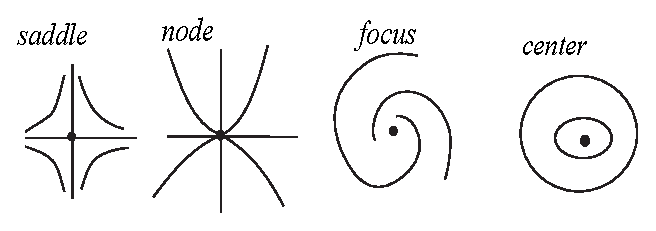
\includegraphics [scale=1.3]{jtr217}
	\caption{Non-degenerate singular points.}
	\label{fig:2.17}
\end{figure}

As already stated in Definition \ref{def:2.1}, the phase portrait of the vector field $v (x)$ on the plane is the split of the plane $\mathbb{R}^{2}$ into the phase curves of that field. The phase portrait elements are: singular points, closed phase curves, separatrix of singular points and behavior on infinity. We will briefly discuss them.

\subsection{Singular points}
They are divided into elementary and non-elementary. The elementary singular points can be subdivided into non-degenerated and degenerate ones.

\begin{definition}
	The equilibrium point $x_0$ of the vector field $v (x)$, $x \in \mathbb{R}^n$, is called \textbf{non-degenerated} if $\det \frac{\partial v}{\partial x}(x_{0})\not=0.$
	
	The equilibrium point $x_0$ of the vector field $v (x)$, $x \in \mathbb{R}^n$, is called \textit{elementary} if at least one of the eigenvalues of the matrix $A=\frac{\partial v}{\partial x}(x_{0})$ is nonzero. In this case, the point $ x_ {0} $ is:
	\begin{itemize}
		\item a \textbf{saddle}, if $\lambda _{1}<0<\lambda _{2}$ for the eigenvalues $\lambda _{1,2}$ of the matrix $A$;
		\item a \textbf{stable node} (respectively an \textbf{unstable node}), if $\lambda _{1},\lambda _{2}<0$ (respectively $\lambda _{1},\lambda _{2}>0$);
		\item a \textbf{stable focus} (respectively \textbf{unstable focus}), if $\lambda _{1,2}\in \mathbb{C}\setminus \mathbb{R}$ and $\textrm{Re}\lambda _{1,2}<0$ (respectively  $\textrm{Re}\lambda _{1,2}>0)$;
		\item a \textbf{saddle-node}, if $\lambda _{1}=0$, $\lambda _{2}\not=0.$
	\end{itemize}
\end{definition}

Local phase portraits surrounded by elementary singular points defined above are shown in Figures \ref{fig:2.17} and \ref{fig:2.18}.

\begin{remark}
	In the case of $\lambda _{1,2}\in i\mathbb{R}\setminus 0$, i.e., purely imaginary values, the critical point $x_0$ may be a stable or unstable focus (more precisely, \textbf{weak focus}) or \textbf{center}; see Proposition \ref{prop:2.11} above.
\end{remark}

\begin{remark}
	The concept of saddle-node given above is quite wide. The point is that we can have the following model situations
	\begin{eqnarray}
	\dot{x} &=&x^{2k},\text{ \ \ }\dot{y}=\pm y,  \label{2.13} \\
	\dot{x} &=&\pm x^{2k+1},\text{\ \ \ }\dot{y}=\pm y.  \label{2.14}
	\end{eqnarray}
	In Section \ref{sec:3.3} below, formulas \eqref{2.13} - \eqref{2.14} will be more justified. When $\dot{x}=x^{s}$ and $ s>2$, then the saddle-node is somewhat degenerated; we say that it has \textit{codimension} $s-1$.
	
	From the topological point of view, the local phase portrait does not depend on $ k$. These portraits are shown in Figure \ref{fig:2.18}.
	
	\begin{figure}[!ht]
		\centering
		\includegraphics [scale=1]{jtr218}
		\caption{Saddle-node.}
		\label{fig:2.18}
	\end{figure}
\end{remark}

\begin{remark}(Non-elementary singular points).
	Let us remind that here we have $\lambda _{1}=\lambda _{2}=0.$ Unfortunately, there is no satisfactory classification of such singularities. But there is an effective method of researching them. This is the method of \textit{blowing-up singularities} (or solving singularities).
	
	It consists of a simple operation of introducing the polar coordinates $ \left (r, \varphi \right) $ on the plane. So if we have, for example,
	\begin{equation}
	\label{2.15}
	\dot{x}=ax^{2}+bxy+cy^{2}+\ldots ,\text{ \ }\dot{y}=dx^{2}+exy+fy^{2}+\ldots
	,
	\end{equation}
	in the polar variables we get
	\begin{equation}
	\label{2.16}
	\dot{r}=r^{2}\left( P(\varphi )+O(r)\right) ,\text{ \ \ }\dot{\varphi}%
	=r\left( Q(\varphi )+O(r)\right) ,
	\end{equation}
	where
	\begin{eqnarray*}
		P &=&a\cos ^{3}\varphi +(b+d)\cos ^{2}\varphi \sin \varphi +(c+e)\cos
		\varphi \sin \varphi +f\sin ^{3}\varphi , \\
		Q &=&d\cos ^{3}\varphi +(e-a)\cos ^{2}\varphi \sin \varphi +(f-b)\cos
		\varphi \sin \varphi -c\sin ^{3}\varphi .
	\end{eqnarray*}
	Note that the right side of the equation \eqref{2.16} will disappear at $r = 0$. Let's divide these right-hand sides by $r$; in the area $r> 0$, the phase portrait will not change, but the `velocity' of the point along the phase curve will be different, but not zero (it could happen that $Q(\varphi )\equiv 0$, but then we divide by $r^2$). This is so-called orbital equivalence, as described below.
	
	But after this operation we get a vector field on the cylinder $\left\{ \left( r,\varphi \right) \right\} \simeq \mathbb{R}\times \mathbb{S}^{1}$ (for which we have an important part $\left\{ r\geq 0\right\} $), with isolated singular points on the circle $r = 0$. If the coefficients $a,\ldots ,f$ are typical, these singular points are already non-degenerated, i.e., elementary.
	
	Otherwise we repeat the procedure of blowing-up (combined with division) in the neighborhood of each non-elementary singular point $r = 0$, $\varphi =\varphi _{0}$ (with new coordinates $x=\varphi -\varphi _{0}$, $y=r$). It turns out that if the original vector field \eqref{2.15} is analytic, then after the finite number of such blows we get a vector field on a surface $M$ with elementary singular points. (This is a difficult statement, after which I refer to my book \textquotedblleft The monodromy group\textquotedblright\ \cite{Zol2}.)
\end{remark}

\begin{figure}[!ht]
	\centering
	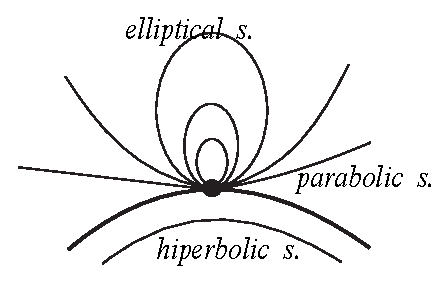
\includegraphics [scale=1.4]{jtr219}
	\caption{Sectors.}
	\label{fig:2.19}
\end{figure}

In the case of non-elementary singular points, its surroundings can be often divided into sectors: \textit{hyperbolic, parabolic and elliptical}. They are illustrated in Figure \ref{fig:2.19}. There is a theory associated with them, which we will not deal with. For interested readers refer to P. Hartman's \cite{Hart}.

\subsection{Closed phase curves}
They correspond to the periodic solutions (and trajectories) and were discussed in detail in the previous section.

\subsection{Separatrix of singular points}
\begin{definition}
	\textbf{Separatrix of a singular point} $x_0$ of the vector field $v (x)$ is how is called the phase curve of that field which `tends' to $x_0$ under a certain limit direction among such curves.
\end{definition}

For example, for the saddles, separatrices there are components of the `perforated' manifolds, stable $ W ^ {s} \setminus x_ {0} $ and unstable $ W ^ {u} \setminus x_ {0} $; in total we have four separatrices.

In the general case, when we have a division into hyperbolic, elliptical and parabolic sectors, separatrices exist at the edges of hyperbolic sectors.

\begin{remark}
	An important element of the phase portrait of a vector field is the `fate' of the second end of the separatrix $L$.
	
	It can land a different singular point $x_1$, usually in its parabolic sector. But it can also wind up on a focus. A special case is when $L$ is a separatrix for both $x_0$ and for $x_1$; then we have to deal with the so-called \textit{separatrix connection}.
	
	The other end of the separatrix can also wind up on a limit cycle.
	
	A special case, and quite exploited in the theory of  Dynamic Systems is the case when the other end of the separatrix $L$ lands at the same point $x_0$. We have then the so-called \textit{separatrix loops}. More on this topic will be found in \cite{ALG1} and \cite{ALG2}.
\end{remark}

\subsection{Behavior on infinity}

There are multiple plane compactifications in $\mathbb{R}^{2}$. One of them is the so-called \textit{Poincaré's compactification} (or Poincaré's plane). It consists in complementing the plane with a circle by adding all `directions of infinity'. Poincaré's plane is diffeomorphic to the disk: $\mathbb{R}^{2}\cup \mathbb{S}^{1}\simeq D^{2}$ (see Figure \ref{fig:2.20}).\footnote{In mathematics more widespread is the using the projective plane $\mathbb{RP}^{2}$. The difference between Poincaré's compactification is that, in the projective plane, two antipodal directions are equivalent in infinity. Unfortunately, the projective plane is a non-oriented variety and can not be drawn (in contrast to the Poincaré's plane).}

Poincaré's compactification is useful for studying the behavior of the phase curves of polynomial vector fields, i.e., the systems $\dot{x}=P(x,y),$ $\dot{y}=Q(x,y)$, whose right hand $P$ and $Q$ are polynomials.

Then in the neighborhood of the circle in infinity you can introduce the polar coordinate type
$$
x=\frac{1}{z}\cos \varphi ,\text{ \ \ }y=\frac{1}{z}\sin \varphi .
$$
We get the character set
$$
\dot{z}=\frac{1}{z^{k}}\left( A(\varphi )+O(z)\right) ,\text{ \ \ }\dot{%
	\varphi}=\frac{1}{z^{l}}\left( B(\varphi )+O(z)\right) ,
$$
i.e., with the pole in the set $\left\{ z=0\right\} $ (circle in infinity). Multiplying the right side by $z^{\min \left( k,l\right)}$, which leads to an orbital equilibrium in the domain $z>0$, we get an accurate vector field in the neighborhood of the infinity circle.

Let us note that the singular points $z=0,$ $\varphi =\varphi _{0}$ of the new field correspond to the situation where any phase curve of the system $\dot{x}=P,$ $\dot{y}=Q$ tends to infinity (at $t\rightarrow +\infty $ or at $t\rightarrow -\infty$) under the boundary of the direction $ \varphi _ {0}$.

\begin{figure}[!ht]
		\centering
		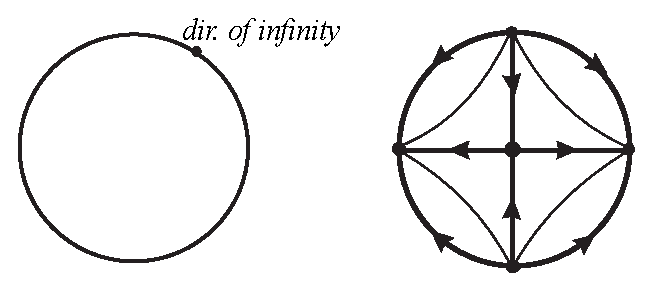
\includegraphics [scale=1]{jtr220}
		\caption{Poincaré plane.}
		\label{fig:2.20}
\end{figure}

\begin{example}
	The linear vector field $\dot{x}=x,$ $\dot{y}=-y$ leads to a phase vector in the Poincaré plane as shown in Figure \ref{fig:2.20}.
\end{example}

\subsection{Orbital equivalence}

\begin{definition}
	Two vector fields $v (x)$ on $M$ and $w (y)$ on $N$ are \textbf{orbitally equivalent} if they have the same phase portraits from a topological point of view. It means, there is a homeomorphism $h:M\longmapsto N$ such that $h ($phase curve $v) = ($phase curve $w)$.
	The vector field $v (x)$ on $M$ is \textbf{orbitally structurally stable}, if every field $w(x)$ on $M$ sufficiently close to the field $v$ (in the appropriate topology) is orbitally equivalent to $v$.
\end{definition}

It is easy to see that, the above definition of orbital equivalence and orbital structural stability is weaker than the definition of equivalence and structural stability given in Definition \ref{def:1.24}.

Thus, the Hartman-Grobman's Theorem (Theorem \ref{theo:1.23}) and the following Proposition \ref{prop:1.25} show that two vector fields in the neighborhood of hyperbolic singular points with the same dimensions of a stable and unstable variety are orbitally equivalent. They are also orbitally structurally stable.

Below, without proof, we provide the necessary conditions for the orbital structural stability of a vector field on the plane.

\begin{theorem}\label{theo:2.43}
	If the field $v (x)$ in the area $U\subset \mathbb{R}^{2}$ is orbitally structurally stable, then:
	\begin{enumerate}[(i)]
		\item its singular points are hyperbolic,
		\item its closed phase curves are hyperbolic limit cycles,
		\item there are no separatrix connections.
	\end{enumerate}
	Moreover, if the area $U$ is compact (e.g. Poincaré plane), then the above conditions for orbital structural stability are also sufficient.
\end{theorem}

\subsection*{Tasks}
\begin{task}
	Calculate the solution of the system $\dot{x}=y,$ $%
	\dot{y}=-\sin x$ (mathematical pendulum) with the initial condition $%
	x(0)=0,$\ $y(0)=2$ corresponding to $H = 1$.
\end{task}

\begin{task}
	Similarly to the mathematical pendulum, find the first integral and sketch the phase curves for the \textit{Duffing system}
	$$
	\dot{x}=y,\text{ \ }\dot{y}=-x+x^{3}.
	$$
	Calculate the solution with the initial condition $x(0)=0,$ $y(0)=1/%
	\sqrt{2}$.
\end{task}

\begin{task}
	Calculate $\dot{r}$ and in $\dot{\varphi}$ Example \ref{example:2.4}.
\end{task}

\begin{task}
	Show that the value of the matrix $A$ in the transformation of Poincaré return $f (z) = Az +\ldots$ does not depend on the choice of cutting $S$ to the periodic orbit $\gamma .$
\end{task}

\begin{task}
	Prove formula \eqref{2.4}.
\end{task}

\begin{task}
	Calculate the coefficient $a_1$ in formula \eqref{2.6}.
\end{task}

\begin{task}
	Assuming that on the right side of the equation \eqref{2.7} there are only square terms (i.e. $D = E =\ldots = 0$) and that $c_3 = 0$, calculate $c_5$.
\end{task}

\begin{task}
	Show that for a linear vector field the number of limit cycles is 0.
\end{task}

\begin{task}
	Show that the $\omega$-limit set $\omega(x)$ for the stream $\left\{ g^{t}\right\} $ is closed and invariant, i.e., $g^{t}\left( \omega (x)\right) =\omega (x)$.
\end{task}

\begin{task}
	Show that in the proof of Theorem \ref{theo:2.19}, the consecutive points $x_j$ of the trajectory $\Gamma(x)$ of the point $x$ with the cutting $S$ form a monotonic sequence, as in Figure \ref{fig:2.7}.
\end{task}

\begin{task}
	Show that the vector field \eqref{2.11} has the property that the square of the radius $r^{2}=x^{2}+y^{2}$ grows along the solution for small $r$.
\end{task}

\begin{task}
	Calculate the index in $(0, 0)$ for the following fields:
	\begin{enumerate}[(a)]
		\item $\dot{x} = x^{3}-3xy^{2},\text{ \ }\dot{y}=y^{3}-3x^{2}y$
		\item $\dot{x} = y+x^{2},\text{ \ \ }\dot{y}=x^{3}$
	\end{enumerate}
\end{task}

\begin{task}
	Show that $i_{0}v=\textrm{sign}\det A$ for the field germ $\dot{x}=Ax+\ldots $ in $\left( \mathbb{R}^{n},0\right) $ such that $\det A\not=0.$ Note: the case of $n> 2$ is a task with an asterisk.
\end{task}

\begin{task}
	Show that the vector field $\dot{x}=1-xy,$ $%
	\dot{y}=x$ does not have limit cycles.
\end{task}

\begin{task}
	Show that the characteristic exponent of the periodic orbit defined in Definition \ref{def:2.27} is well defined.
\end{task}

\begin{task}
	Complete the analysis of the Jouanolou system in the case of the odd $s$.
\end{task}

\begin{task}
	Calculate \textrm{div}$\left( \frac{1}{f}v\right) $ in Van der Pol's analysis.
\end{task}

\begin{task}
	Sketch a phase portrait (in $\mathbb{R}^{2}$) for the system $\dot{x}=1+x^{2}-y^{2},$\ $\dot{y}=x+x^{2}-2xy.$
\end{task}

\begin{task}
	Sketch a phase portrait for the system $\dot{x}%
	=y^{2}-4x^{2},$ $\dot{y}=4y-8.$
\end{task}

\begin{task}
	Sketch a phase portrait for the equations $\dot{z}=z^{2}$ and $\dot{z}=\bar{z}^{2},$ where $z=x+iy\in \mathbb{C}\simeq
	\mathbb{R}^{2}.$
\end{task}

\begin{task}
	Consider the vector field $v (x, y)$ of form \eqref{1.2}, i.e., $\dot{x}=y+x^{2},$ $\dot{y}=-2x^{3}-4xy-y(x^{2}+y^{2})^{2};$ we want to show that the phase portrait of this circuit is as in Figure \ref{fig:1.2}.
	\begin{enumerate}[(a)]
		\item Let's start with the simpler vector field $v_{0}(x,y)$ given by the system\begin{equation}
		\label{2.17}
		\dot{x}=y,\ \ \ \dot{y}=-2x^{3}-4xy.
		\end{equation}
		Make a substitution with $z=x^{2}$ to sketch its phase portrait and show that in the neighborhood $x=y=0$ it is of the same quality as in Figure \ref{fig:1.2} (only has a larger elliptic sector). Also indicate that the parabola $y=-x^{2}$ is invariant for the field \eqref{2.17} and contains separators at the hyperbolic boundary.
		\item Using double blow show, the fields $v$ and $v_0$ have the same phase portrays in the neighborhood $x = y = 0$.
		\item Show that adding the component $-y\left(
		x^{2}+y^{2}\right) ^{2}\frac{\partial }{\partial y}$ of the field $v_{0}$ causes that in the area $U=\left\{ y\geq -x^{2}\right\} $ (i.e. the whole elliptic sector for $v_{0}$ with the edge) we divide the phase curves of the field $v_{0}$ by the angle, and so that the phase curves of the field $v$ move more toward the center of the coordinate system. In conclusion, all points in the area $U$ go to $(0, 0)$ under the influence of the phases $\left\{ g_{v}^{t}\right\}_{t>0}$.
		\item Show that the remaining points from the neighborhood of $(0, 0)$ either lie in the stable separatrix of the point $(0, 0)$ (i.e., for $v$) or enters the domain $U$ after the end of time under the influence of the stream $g_{v}^{t}.$
	\end{enumerate}
\end{task}
\chapter{Bifurcation theory}
\section{Versality}

According to Theorem \ref{theo:2.43}, typical vector fields on a compact 2-dimensional manifold $M$ are orbitally structurally stable. If we denote by $\mathcal{X}$ the infinitely dimensional space of all vector fields on $M$ (given a class and with a suitable topology that we will not talk about), then the subset $\Sigma$, called the \textit{bifurcation set}, of the space $\mathcal{X}$  consisting of fields that are not orbitally structurally stable, should have codimension $\geq 1$. It should be expected that this subset $\Sigma$ is generally smooth, but may have irregular points (as in Figure \ref{fig:3.1}). The last points should correspond to vector fields which have more complex singularities than those corresponding to typical points from $\Sigma$.

\begin{figure}[!ht]
	\centering
	\includegraphics [scale=1]{jtr31}
	\caption{Bifurcation set.}
	\label{fig:3.1}
\end{figure}

If we randomly select a field from $\mathcal{X}$, then with probability 1 it will be outside of the set $\Sigma$. But the whole family $\left\{ v_{\lambda }\right\} _{\lambda \in \mathbb{R}}$ of vector fields is a curve in $\mathcal{X}$ and can already cross the hypersurface $\Sigma$. We also expect that, for a typical family, the corresponding curve will cross the $\Sigma$ hypersurface at the angle and at typical points of this hyperplane (see Figure \ref{fig:3.1}).

The bifurcation theory is concerned with the study of both the geometry of the bifurcation set $\Sigma$ and the behavior of the multi-parameter families of the vector fields. We will limit ourselves to 1-parameter families.

Pay attention to one more aspect of this situation. In space $\mathcal{X}$ there exists a group $\mathcal{G}$ of orbital equivalence and the subdivision $\Sigma$ is invariant in relation to that action. It is therefore necessary to link the analysis of 1-parameter families $\left\{ v_{\lambda }\right\} $ to the action of group $\mathcal{G}$. V. Arnold in \cite{Ar2} introduced once and for all the definitions in this field and the following definitions come from him.\footnote{This philosophy also works in other general situations. For example, where $\mathcal{X}$ is a space of functions $f$ on manifolds, and $\mathcal{G}$ is the group of diffeomorphisms $h$ of manifold with the function $f\longmapsto f\circ h.$ Likewise, $\mathcal{X}$ can be a space of the diffeomorphisms $f$ of the manifold $M$ and the group $\mathcal{G}$ of the diffeomorphisms on $M$ can be obtained by composition: $f\longmapsto h\circ f\circ h^{-1}$.}

\begin{definition}
	The two families $\left\{ v_{\lambda }\right\} _{\lambda
	\in J}$ and $\left\{ w_{\lambda }\right\} _{\lambda \in J}$, $J\subset \mathbb{R}$, of the vector fields on $M$ are \textbf{orbitally equivalent} if for every $\lambda \in J$, the fields $v_{\lambda }(x)$\ and $w_{\lambda }(x)$ are orbitally equivalent by the homeomorphism $h (x)$, which depends in a continuous manner on the parameter $\lambda$.
	
	We say that the family $\left\{ w_{\nu }\right\} _{\nu \in K}$ is \textbf{induced} from $\left\{ v_{\lambda }\right\} _{\lambda \in J}$ if there exists a continuous mapping $\varphi :K\longmapsto J$ such that
	$$
	w_{\nu }=v_{\varphi (\nu )}.
	$$
	
	The family $\left\{ v_{\lambda }\right\} _{\lambda \in \left( \mathbb{R}%
	,0\right) },$ with the given $v_{0}$, is \textbf{versal} if any other family $\left\{ w_{\nu }\right\} _{\nu \in \left( \mathbb{R}%
	,0\right) }$ with $w_{0}=v_{0}$ is orbitally equivalent to a family induced from the family $\left\{ v_{\lambda }\right\} .$
\end{definition}

\begin{example}
	Family $\dot{x}=\nu ^{2}+x^{3}$ is induced from family $\dot{x}=\lambda +x^{3}$ with the help of the change of variables $\lambda
	=\varphi (\nu )=\nu ^{2}.$
\end{example}

\begin{example}\label{example:3.3}
	Let's model the vector field family
	\begin{equation}
	\label{3.1}
	\dot{x}=v_{\lambda }(x)=\lambda +x^{2}.
	\end{equation}
	The corresponding phase portraits are shown in Figure \ref{fig:3.2}.
	
	Let us now take any family of form
	\begin{equation}
	\label{3.2}
	\dot{x}=w_{\mu }(x)=x^{2}+\mu \tilde{w}(x,\mu )=:f(x,\mu ),
	\end{equation}
	where $\tilde{w}(x,\mu )$  is a smooth function in a neighborhood of $x=\mu
	=0 $. We claim that 
	\begin{figure}[!ht]
		\centering
		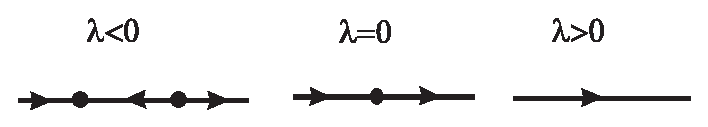
\includegraphics [scale=1]{jtr32}
		\caption{Phase portraits.}
		\label{fig:3.2}
	\end{figure}

	\emph{for every $\mu$ the vector field $w_{\mu }$ has either 1 or 2 or 0 singular points in a neighborhood of $x = 0$.}\\
	To see this, consider the equation
	$$
	g(x,\mu )=0,
	$$
	where $g(x,\mu )=f_{x}^{\prime }(x,\mu ).$ Since $f_{xx}^{\prime
	\prime }(0,0)\not=0,$ then $g_{x}^{\prime }(0,0)\not=0,$ and from the Implicit Function Theorem there exists a smooth function $\psi (\mu )$ such that the equation $g(\psi (\mu ),\mu )\equiv 0$ is satisfied. This means that point
	$$
	x_{\mu }=\psi (\mu )
	$$
	\begin{figure}[!ht]
		\centering
		\includegraphics [scale=1]{jtr33}
		\caption{Right-side graphs.}
		\label{fig:3.3}
	\end{figure}
	is the point of the local minimum of the function $w_{\mu }=f(\cdot ,\mu ):\ \frac{dw_{\mu }}{dx}(x_{\mu })=0.$ We have three possibilities for the value of the field $w_{\mu }$ at point $x_{\mu }$: (i) $w_{\mu }(x_{\mu })=0$, (ii) $w_{\mu }(x_{\mu })<0$, (iii) $w_{\mu
	}(x_{\mu })>0$. In case (i) the field $w_{\mu }$ has no equilibrium points (saddle-node type), in case (ii) the field $w_{\mu }$ has two hyperbolic equilibrium points and in case (iii) there is one equilibrium point (see Figure \ref{fig:3.3}).

	So for every $\mu $, the phase portrait of the field $w_{\mu }$ is topologically equivalent to the phase portrait of the field $v_{\lambda }$ for the corresponding $\lambda$. There is a natural question of whether we can obtain $\lambda =\varphi (\mu )$ and homeomorphisms $h_{\mu }$ that realize an orbital equivalence of $w_{\mu }$ with $v_{\varphi (\mu)}$ so that the dependence on $\mu $ is continuous. It turns out that yes; it means that the family \eqref{3.1} is versal.

	\begin{figure}[!ht]
		\centering
		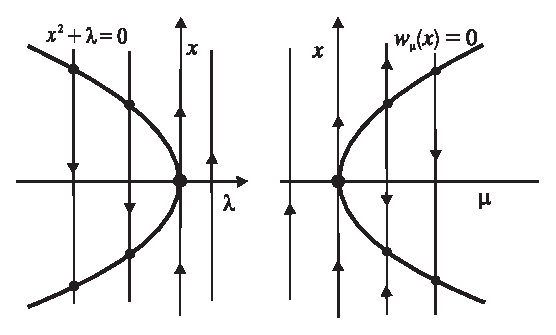
\includegraphics [scale=1.2]{jtr34}
		\caption{Model of family bifurcation and typical family bifurcation.}
		\label{fig:3.4}
	\end{figure}

	In order to convince ourselves, let us first consider the case where
	\begin{enumerate}[(a)]
		\item $\frac{\partial f}{\partial \mu }(0,0)\not=0$ in \eqref{3.2}. Then the curve of the equilibrium point
		$$
		\Gamma :w_{\mu }(x)=f(x,\mu )=0
		$$
		of the field $w_{\mu }$ on the plane of the variables $x,\mu $ is `vertical' and the homeomorphic with a parabola (see Figure \ref{fig:3.4}). Also the parabola is the curve of the equilibrium points $\Delta =\{\lambda =-x^{2}\}$ for the field $v_{\lambda }$.
		
		Depending on the sign of $f_{\mu }^{\prime }(0,0)$ we put $\varphi
		\left( \mu \right) =\mu $ or $\varphi
		\left( \mu \right) =-\mu $; so we can assume that both `parabolas' are oriented the same way. In this case, the homeomorphic constructions $h_{\mu }$, i.e., the homeomorphism of the plane $$
		\left( \mu ,x\right) \longmapsto \left( \mu ,h_{\mu }(x)\right) ,
		$$
		start with the construction of the homeomorphism between the curves of the equilibrium points: $\Gamma \longmapsto \Delta $. Then we extend this homeomorphism continuously to the plane, so that the vertical sections (at $\mu =\textrm{const}$) outside the equilibrium points go to the corresponding vertical sections. It is clear that it is possible to do so.
		\item In the degenerate case, when $f_{\mu }^{\prime }(0,0)=0,$ the curve of the equilibrium points $\Gamma =\{f=0\}$ can be very complex (see Figure \ref{fig:3.5}). But we know that from every straight vertical $\mu =\textrm{const}$ the curve has at most two points of the shear. Let us denote the intersection of $\Gamma _{\mu }$ and $\Gamma$ with such a straight line. Thus the parabolic construction $\mu \longmapsto	\varphi (\mu )$ lies in the parameters $\mu$, for which $\#\Gamma _{\mu }=2$ have gone to the left of $\lambda =0$ and the parameters $\mu$, for which $\#\Gamma _{\mu }=0$ have gone to the right of $\lambda =0$ (with continuity). Then, repeating arguments from case (a), we construct a first the continuous transformation $\left( \mu ,x\right) \longmapsto (\varphi (\mu ),h_{\mu }(x))$ between the $\Gamma $ and $\Delta $ curves and then extend them in a continuous manner with the preservation of the vertical.
	\end{enumerate}
	This also proves that the family $v_{\lambda }(x)=\lambda +x^{2}$ is versal.
	\begin{figure}[!ht]
		\centering
		\includegraphics [scale=1]{jtr35}
		\caption{Bifurcation of an atypical family.}
		\label{fig:3.5}
	\end{figure}
\end{example}

\section{Transversality}

A mathematical tool for the exact formulation of bifurcation theory and corresponding theorems is the theory of transversality formulated by the French mathematician R. Thom.

Let $M$ be a $n$-dimensional manifold and let $B\subset M$ be its $k$-dimensional submanifold. In addition, let $A$ be a $m$-dimensional manifold and 
$$
f:A\longmapsto M
$$
will be a differential mapping (with sufficient class of differentiability). In the case of compact manifolds $A$ and $M$ in the space $C^{k}(A,M)$ the natural topology is introduced (which will not be squeezed).
 
 \begin{definition}
 	We say that \textbf{the mapping $f$ is transversal to the submanifold $B$}, if for every point $x\in A$ such that $y = f (x) \in B$, the following property is hold
 	$$
 	f_{\ast }T_{x}A+T_{y}B=T_{y}M.
 	$$
 	When $A\subset M$ is a submanifold and $f=id|_{A}$ is a embedding, then we say that \textbf{$A$ is transversal to $B$} if the property
 	$$
 	T_{y}A+T_{y}B=T_{y}M
 	$$
 	is hold for every point $y\in A\cap B$. We have the standard symbols
 	$$
 	f\pitchfork B\text{ \ \ and \ \ }A\pitchfork B
 	$$
 	for transversal properties.
 \end{definition}

\begin{figure}[!ht]
	\centering
	\includegraphics [scale=1]{jtr36}
	\caption{Transversal and non-transversal curves in the plane.}
	\label{fig:3.6}
\end{figure}

\begin{example}
	\begin{enumerate}[(a)]
		\item Let $M=\mathbb{R}^{2}$ and $A\subset M$ and $B\subset M$ be smooth curves. Then  $A\pitchfork B$ when curve $A$ crosses curve $B$ under a non-zero angle (see Figure \ref{fig:3.6}).
		\item Let $M=\mathbb{R}^{3}$, $A\subset M$ be a curve and $B\subset M$ be a submanifold. Figure \ref{fig:3.7} shows cases of transversality and non-transversality.
		\item The case $M=\mathbb{R}^{3}$ and two surfaces $A\subset M$, $B\subset M$ is shown in Figure \ref{fig:3.8}.
		\item When $M=\mathbb{R}^{3}$ and $A\subset M$, $B\subset M$ are curves, then $A\pitchfork B$ if and only if the curves are disjoint.
		\item Let $M=\mathbb{R}^{2}=\left\{ \left( x,y\right) \right\}$, $A = \mathbb{R}^{1}$ and $B=\left\{ x=0\right\} $ and let $f:A\longmapsto M$  be given by the formula $f(t)=(t^{3},0)$. Of course $f(t)\in B$ is only for $t = 0$. But then $f_{\ast }(0)=f^{\prime }(0)=0$. So $f_{\ast		}T_{0}A+T_{(0,0)}B=T_{(0,0)}B\simeq B\not=T_{(0,0)}M$. This example shows the importance of the transversality properties of the mapping to a submanifold.
	\end{enumerate}
\end{example}

\begin{figure}[!ht]
	\centering
	\includegraphics [scale=1]{jtr37}
	\caption{Transversal and non-transversal curve and surface in the space.}
	\label{fig:3.7}
\end{figure}

\begin{figure}[!ht]
	\centering
	\includegraphics [scale=1]{jtr38}
	\caption{Transversal and non-transversal surfaces in the space.}
	\label{fig:3.8}
\end{figure}

The following fundamental theorem follows from Thom.\footnote{Thom's Transcendence Theorem, as well as its generalization given below, were an important part of his Catastrophe theory. This theory includes, in part, the theory of peculiarity of mappings and functions as well as the theories of bifurcation of dynamic systems.

It is worth adding that, in the case of the generalization of Thom's Theorem on the case of non-compact manifolds, special topologies (so called Whitney topologies) are introduced in the $C^k$ class projection space.}

\begin{theorem}\emph{(Thom).}\label{theo:3.6}
	Let $M$, $A$ and $B$ be fixed compact manifolds as above. Then the set of maps $f:A\longmapsto M$ that are transversal to $B$ is open and dense in $C^r (A,M)$.
	
	This means that, on the one hand, if the mapping $f_0$ is transversal to $B$, then any mapping $f_{\varepsilon}$ is transversal to $B$, and, on the other hand, if $f_0$ is not transversal,  then there exists a map $f_{\varepsilon}$ arbitrarily close to it that is already transversal to $B$ .
	
	\begin{proof}
		It is easy to see that we can limit ourselves to the local situation when $A\subset \mathbb{R}^{m}$ and $M\subset \mathbb{R}^{n}$ are open subsets and
		$$
		B=\left\{ y_{1}=\ldots =y_{n-k}=0\right\} \cap M
		$$
		is (locally) a subspace of codimension $n-k$ (Task 3.16).
		
		Then $f(x)=\left( f_{1}(x),\ldots f_{n}(x)\right) $ and
		$$
		T_{y}B=\left\{ q\in \mathbb{R}^{n}:q_{1}=\ldots =q_{n-k}=0\right\} \subset
		T_{y}M=\mathbb{R}^{n}.
		$$
		If $f(x_{0})\in B$, i.e., $f_{1}(x_{0})=\ldots f_{n-k}(x_{0})=0$, then $f$ is transversal at $x_0$ to $B$ if and only if the vectors $f_{\ast }\partial _{x_{1}},\ldots ,f_{\ast }\partial _{x_{m}}$ together with the vectors $\partial _{yn-k+1},\ldots \partial _{y_{n}}$ expand $\mathbb{R}^{n}$. (Here $\partial _{x_{j}}$ and $\partial _{y_{k}}$ are the base vectors in $\mathbb{R}^{m}$ and $\mathbb{R}^{n}$ respectively.) In addition, the projections of the $f_{\ast }\partial _{x_{j}}$ vectors on the quotient space $T_{y}M/T_{y}B\simeq \mathbb{R}^{n-k}$ expand the space. This means that matrix$$
		C=
		\begin{pmatrix}
		\partial f_{1}/\partial x_{1} & \ldots  & \partial f_{1}/\partial x_{m} \\
		\vdots  & \ddots  & \vdots  \\
		\partial f_{n-k}/\partial x_{1} & \ldots  & \partial f_{n-k}/\partial x_{m}%
		\end{pmatrix}
		$$
		has rank $\textrm{rk\,}C\geq n-k$.
		
		We have two possibilities:
		\begin{enumerate}[(i)]
			\item $m<n-k$ and then the rank is smaller than $n-k$, which is impossible,
			\item $m\geq n-k$ (then the property of \textrm{rk} $C\geq n-k$ is an open condition in the matrix space).
		\end{enumerate}
	In the case (i) transversality means that there is no $f (A)$ in $B$ and that it is an open condition in the mapping space. Also in case (ii) it is not difficult to show that the condition of transversality is open (Task 3.13).
	
	To prove the inherent nature of transversality we need to introduce additional concepts (Task 3.14).
	
	In case (ii) let us consider the local mapping $g:A\longmapsto R^{n-k},$%
	$$
	g(x)=(f_{1}(x),\ldots ,f_{n-k}(x)).
	$$	
	Recall (see Definition \ref{def:3.7} below), where $x_0$ is the critical point for $g$ if rk$\frac{\partial g}{\partial x}(x_{0}) = $ rk$C<n-k,$ and the value $g (x_0)$ is called the critical value for $g$. We will use the classical Sard Theorem (Theorem \ref{theo:3.8} below), which ensures that the set of critical values for $g$ is `rare'. According to Task 3.15 $f\pitchfork B$ iff 0 is not a critical value for $g$. Let $z$ be a non-critical value for $g$ and close to zero. We will distort the mapping $f=(g,h)$ in the following way
	$$
	f_{\varepsilon }(x)=(g(x)-z,h(x)).
	$$
	It is easy to see that $f_{\varepsilon }$ is transversal to $B$ (Task 3.16).
	\end{proof}
\end{theorem}

\begin{definition}\label{def:3.7}
	Let $h:\mathbb{R}^{m}\longmapsto \mathbb{R}^{l}$ be a differentiable mapping. We say that $x_0$ is a \textbf{critical point} for $h$ if rk $\frac{\partial h}{\partial x}(x_{0})$ is not maximal. The value $h(x_0)$ at the critical point is called the \textbf{critical value} for $h$.
\end{definition}

\begin{theorem}\emph{(Sard).}\label{theo:3.8}
	The set of critical values for the differential mapping $h:\mathbb{R}^{m}\longmapsto \mathbb{R}^{l}$ of a sufficiently high class of smoothness has zero Lebesgue measure.
	\begin{proof}[Idea of the proof]
		Consider the case of $m = l = 1$. It is not excluded that the critical values for $g$ can form a set of gestures in $\mathbb{R}$. We can, however, cover every critical point $x_j$ with a section $I_{j}$ of width $\left\vert I_{j}\right\vert \leq \varepsilon $ for any small $\varepsilon $. Since $g^{\prime }(x_{j})=0,$ then the length of the image $g(I_{j})$ of that segment will be the width of the order $ O(\varepsilon ^{2})=O(\varepsilon )\left\vert I_{j}\right\vert $ (see Figure \ref{fig:3.9}). Therefore,
		$$
		\left\vert g\left( \bigcup I_{j}\right) \right\vert \leq O(\varepsilon
		)\cdot \left\vert \bigcup I_{j}\right\vert \leq O(\varepsilon ),
		$$
		tends to zero as $\varepsilon \rightarrow 0.$
		
		The same argument applies to any $m\leq l $ (Task 3.17). When $m>l$ proof is more complicated (with the division of $\mathbb{R}^{m}$ into subsets of the constant order of the matrix $\partial h/\partial x$).
		\begin{figure}[!ht]
			\centering
			\includegraphics [scale=1.3]{jtr39}
			\caption{Sard Theorem.}
			\label{fig:3.9}
		\end{figure}
	\end{proof}
\end{theorem}

The following definition is needed to generalize Thom's Theorem. Let
\begin{equation}
\label{3.3}
f:\mathbb{R}^{m}\longmapsto \mathbb{R}^{n}
\end{equation}
be a mapping sufficiently many times differentiable. With such mapping, we can associate a series of geometric objects. The first is the graph
$$
\left\{ (x,f(x))\right\} \subset \mathbb{R}^{m}\times \mathbb{R}^{n}=:J^{0}(\mathbb{R}^{m}, \mathbb{R}^{m}).
$$
Another graph of the derivative is the graph of the mapping $Df: x\longmapsto
(y,p) = (f(x), \frac{\partial f}{\partial x}(x))$,
$$
\left\{ \left( x,f(x),\frac{\partial f}{\partial x}(x)\right) \right\}
\subset \mathbb{R}^{m}\times \mathbb{R}^{n}\times \mathbb{R}^{m\cdot n}=:J^{1}(\mathbb{R}^{m},\mathbb{R}^{n}).
$$
In general, the graph of mapping of the $r$-th order mapping derivative $x \longmapsto (f(x), Df(x),\linebreak \ldots, D^{r}f(x))$ is a subset (relatively large) of the space denoted by $J^{r}(\mathbb{R}^{m},\mathbb{R}^{n})$.

\begin{definition}
	The $J^{r}(\mathbb{R}^{m},\mathbb{R}^{n})$ spaces are called \textbf{jets spaces of  order $r$} from $\mathbb{R}^{m}$ to $\mathbb{R}^{n}.$ Every mapping of the form \eqref{3.3} is associated with his \textbf{$r$-th jet}
	$$
	x\longmapsto j^{r}f(x)=(x,f(x),Df(x),\ldots ,D^{r}f(x))\in J^{r}(\mathbb{R}%
	^{m},\mathbb{R}^{n}).
	$$
	Analogously, if $A$ and $M$ are manifolds of dimension $m$ and $n$ respectively, it defines the spaces $J^{r}(A,M)$ of the jets mapped from $A$ to $M$, and each different map $f:A\longmapsto M$ is bound to its $r-$th jet $j^{r}f:A\longmapsto J^{r}(A,M).$
\end{definition}

\begin{definition}
	If $C\subset J^{r}(A,M)$ is a submanifold, we say that the mapping $f:A\longmapsto M$ is \textbf{transversal to $C$} (denotation $f\pitchfork C$) when $j^{r}f\pitchfork C.$
\end{definition}

\begin{theorem}\emph{(Thom).} \label{theo:3.11}
	Let $A$, $M$ and $C\subset J^{r}(A,M)$ be fixed. Then the set of mappings $f:A\longmapsto M$, which are transversal to $C$, is open and dense in the set of all such mappings.
	\begin{proof}
		This proof in a large part repeats the proof of Theorem \ref{theo:3.6}. The basic difference lies in the proof of density, more specifically, in the choice of the perturbation. Instead of replacing $f(x)\rightarrow f(x)-z$ (where $z$ is a `small' noncritical value for $f$), it is replaced by $f(x)\rightarrow
		f(x)-z-\tilde{p}(x)-\tilde{q}(x,x)-\ldots -\tilde{s}(x,\ldots x),$ where $\tilde{p}$, $\tilde{q}$, $\ldots ,\tilde{s}$ are `small' linear transformations, homogeneous squares, or homogeneous degrees $r$.
	\end{proof}
\end{theorem}

\begin{example}\label{example:3.12}
	Certain natural conditions for mappings are interpreted as conditions for its transversality in jets. For example, the condition
	$$
	\frac{\partial f}{\partial \lambda }(x,\lambda )\cdot \frac{\partial ^{2}}{%
		\partial x^{2}}f(x,\lambda )\not=0\text{ \ where \ }f(x,\lambda )=\frac{%
		\partial f}{\partial x}(x,\lambda )=0
	$$
	follows from the simultaneous transversality of mapping
	$$
	j^{1}f:\mathbb{R}^{2}=\left\{ \left( x,\lambda \right) \right\} \longmapsto
	J^{1}(\mathbb{R}^{2},\mathbb{R})=\left\{ \left( x,\lambda
	,y,p_{x},p_{\lambda }\right) \right\}
	$$
	to the two submanifolds $$
	C_{1}=\left\{ y=0\right\} \text{ \ and \ }C_{2}=\left\{ y=p_{x}=0\right\} .
	$$
	Indeed, transversality to $C_{1}$ means that $\frac{\partial
	y}{\partial x}=\frac{\partial f}{\partial x}\not=0$ or $\frac{\partial y}{%
	\partial \lambda }=\frac{\partial f}{\partial \lambda }\not=0$ when $y=f(x,\lambda )=0.$
	Meanwhile, transversality to $C_{2}$ means that $\left\vert
	\begin{array}{ll}
	f_{x}^{\prime } & f_{\lambda }^{\prime } \\
	f_{xx}^{\prime \prime } & f_{x\lambda }^{\prime \prime }%
	\end{array}%
	\right\vert \not=0$ where $y=f=0$ and $p_{x}=f_{x}^{\prime }=0.$
\end{example}
\bigskip
In the problems of bifurcation theory always, when conditions of a similar character as in Example \ref{example:3.12} appear, we can assume that either are satisfied with probability 1 or with the same probability can not be satisfied. The second case occurs when $\dim A+\dim C<\dim J^{r}(A,M).$ This is a practical conclusion from Thoma's theorem.

\subsection*{Tasks}
\begin{task}
	In the case of $m\geq n-k$, note that (in the proof of Theorem \ref{theo:3.6}) rk$C\geq n-k$ means rk $C=n-k$. Use the Implicit Function Theorem to show that $f^{-1}(B)\subset A$ in a neighborhood of $x_{0}$ is a submanifold in $A$ of codimension $n - k$. Then show that for any $f_{\varepsilon }$ near to $f$, also $f_{\varepsilon }^{-1}(B)$ is a local submanifold of codimension $n-k$ close to $f^{-1}(B)$. In this case, deduce from the openness of a subset of the matrix of the order $n-k$ in the space of the matrices of dimension $(n-k)\times n$, that $f_{\varepsilon }$ is transversal to $B$ in the neighborhood of $x_0$.
\end{task}

\begin{task}
	Show the local duality of transversal property in the case of $m <n-k$.
	
	Tip: Select the appropriate disturbance $f_{\varepsilon }$ for $f$, which is not transversal to $B$.
\end{task}

\begin{task}
	Show that $f\pitchfork B$ if and only if 0 is not critical for the mapping $g$.
\end{task}

\begin{task}
	Complete the proof of Theorem \ref{theo:3.6}.
	
	Tip: Use the corresponding unity distribution $1=\sum \varphi _{j}(x)$ in $A$ associated with local affine maps in $A$, $M$ and $B$. Local disorder select in the form $f_{\varepsilon}=\left( g-\psi_{k}(x) z_{k}, h(x)\right)$, with the corresponding functions $\psi_{k}(x)$ with a compact support and `small' vectors $z_{k}$. Finally, take advantage of the compactness of $A$.
\end{task}

\begin{task}
	Prove the Sard Theorem for cases $m <l$ and $m = l> 1$.
\end{task}
\section{Codimension 1 bifurcations}\label{sec:3.3}

Bifurcations autonomous vector fields will be divided into local and non-local.

\textbf{Local bifurcation}s occur around the singular point $x = 0$ for the bifurcation parameter value. More precisely, we have a family
$$
\dot{x}=v(x;\mu )
$$%
such that
$$
v(x,0)=Ax+\ldots .
$$
In the case of typical 1-parameter families, the violation of the hyperbolic condition (i.e., $\textrm{Re}\lambda _{j}(A)\not=0$ for all the eigenvalues) occurs in two cases:
\begin{enumerate}
	\item $\lambda _{1}(A)=0$ and $\textrm{Re}\lambda _{j}(A)\not=0$ for $j>1$; this is a \textbf{saddle-node bifurcation}.
	\item $\lambda _{1}=\bar{\lambda}_{2}=i\omega \in i\mathbb{R}\setminus 0$
	and $\textrm{Re}\lambda _{j}\not=0$ for $j>2$; this is a \textbf{birth of the limit cycle bifurcation} or the \textbf{Andronov-Hopf bifurcation}.
\end{enumerate}

We have three \textbf{non-local bifurcations} associated with the periodic orbit $\gamma$ for the field $v (x, 0)$. Let $\lambda _{j}$ be the eigenvalues of part of the linear transformation of Poincaré's return. Recall that the hyperbolic condition for $\lambda _{j}$ denotes that $\left\vert \lambda _{j}\right\vert \not=1$ for all $j$. Thus, typical codimension 1 bifurcations may occur in the following cases:
\begin{enumerate}\setcounter{enumi}{2}
	\item $\lambda _{1}=1$ and $\left\vert \lambda _{j}\right\vert \not=1$
	for $j>1$; this is a \textbf{saddle-node bifurcation for periodic orbit}.
	\item $\lambda _{1}=-1$ and $\left\vert \lambda _{j}\right\vert \not=1$
	for $j>1$; this is a \textbf{period doubling bifurcation}.
	\item $\lambda _{1}=\bar{\lambda}_{2}\in \mathbb{S}^{1}\setminus
	\{1,-1\}$. Here the cases where $\lambda _{1}=e^{2\pi ik/m}$ is an element of degree $m=1$, they are called \textbf{resonances}; in addition, when $m = 3, 4$ we are talking about a \textbf{strong resonance}.
\end{enumerate}

\begin{figure}[!ht]
	\centering
	\includegraphics [scale=1.4]{jtr310}
	\caption{Connection separatrices and loop separatrices.}
	\label{fig:3.10}
\end{figure}

Finally, there are two \textbf{non-local bifurcations} related with the connection separatrices (see Figure \ref{fig:3.10}):
\begin{enumerate}\setcounter{enumi}{5}
	\item \textbf{Separatrix connection} between different saddles.
	\item \textbf{Separatrix loop} of one saddle.
\end{enumerate}

\subsection{Reduction to center manifold and Poincaré-Dulac normal form} \label{subsec:3.3.1}

Let's assume we have the vector field
$$
\dot{x}=v(x)=Ax+\ldots
$$
with the singular point $x = 0$. We can assume that matrix $A$ has diagonal blocks
\begin{equation}
\label{3.4}
A=A^{s}\oplus A^{u}\oplus A^{c},
\end{equation}
where $A^s$ (respectively $A^{u}$ and $A^{c}$) has eigenvalues with $\textrm{Re}\lambda _{j}<0$ (respectively with $\textrm{Re}\lambda _{j}>0$ and with $\textrm{Re}\lambda _{j}=0).$

\begin{theorem}\emph{(Shoshitaishvili).} \label{theo:3.18}
	In the situation above, there is a local homeomorphism $h:\left( \mathbb{R}^{n},0\right) \longmapsto \left( \mathbb{R}^{n},0\right) $ performing a phase portrait of field $v(x)$ for the phase portrait of the following field
	\begin{equation}
	\label{3.5}
	\dot{y}_{1}=-y_{1},\text{ \ }\dot{y}_{2}=y_{2},\text{ \ }\dot{y}%
	_{3}=w(y_{3}),
	\end{equation}
	where
	$$
	w(y_{3})=A^{c}y_{3}+\ldots
	$$
\end{theorem}

The proof of this theorem is technical and complex (see \cite{Ar2}). Therefore, we will not quote it here. For this we will draw from it very practical applications. We also note that this theorem is a generalization of the Hartman-Grobman Theorem.

\begin{definition}
	The submanifold given by the equation
	$$
	W^{c}=\left\{ y_{1}=0,\text{ }y_{2}=0\right\}
	$$
	(in terms of \eqref{3.5}) is called \textbf{center manifold}.
\end{definition}

Shoshitaishvili Theorem says that in the case of non-hyperbolic singular point the `interesting part' of dynamics takes place on the central manifold.

For the family of vector fields $v(x,\mu )$ we can treat $\mu$ as an additional variable, i.e., we have the system
$$
\dot{x}=v(x,\mu ),\text{ \ }\dot{\mu}=0,
$$
to which we apply Theorem \ref{theo:3.18} (with $h(x,\mu )=(h_{0}(x,\mu ),\mu
$). We have the following \textbf{reductions to the center manifold}.

\begin{proposition}
	For the family $\dot{x}=v(x,\mu )$ with $v(x,0)=Ax+\ldots $, $A = A^{s}\oplus A^{u}\oplus A^{c}$, there is a local homeomorphism $(h_{0}(x,\mu ),\mu )$ giving the topological equivalent of this family to the following family
	$$
	\dot{z}=w(z,\mu ),\text{ \ }\dot{z}_{1}=-z_{1},\text{ \ }\dot{z}_{2}=z_{2}.
	$$
\end{proposition}

The very existence of the center manifold $W^{c}$ is a generalization of the Hadamard-Perron Theorem. It is possible to search for it as in Theorem \ref{theo:1.18}. In this case, the center manifold is not uniquely determined; it depends on the choice of field extension (or diffeomorphism) for all $\mathbb{R}^n$.

But there is a way to designate $W^c$ in a formal way. We look at it as a graph
$$
W^{c}=\left\{ x_{1}=f(x_{3}),\text{ \ }x_{2}=g(x_{3}):x_{3}\in E^{c}\right\}
$$
(where the coordinates $(x_1, x_2, x_3)$ are related to the decomposition \eqref{3.4}), which is invariant relative to the field $v (x)$. It turns out that the mappings $f:E^{c}\longmapsto E^{s}$ and $g:E^{c}\longmapsto E^{u}$ have unambiguously defined Taylor series at $x_3 = 0$, $f(x_{3}),g(x_{3})=O(\left\vert x_{3}\right\vert ^{2}).$ On $W^{c}$, which is the parameter called by $x_{3}\in E^{c},$ we obtain the vector field
$$
\dot{x}_{3}=w(x_{3}).
$$
This reduction to $ W ^ {c} $ is called \textbf{Lyapunov-Schmidt reduction}.

Unfortunately, it generally turns out that the dealing series of $f$ and $g$ are divergent (even if $v (x)$ is analytic). This also explains the ambiguity of the $W^c$ in a topological sense.

\begin{example} (Euler).
	Let's consider the system
	$$
	\dot{x}=x^{2},\text{ \ }\dot{y}=y-x^{2}.
	$$
	Here $ W ^ {u} = \left \{x = 0 \right \} $ is an unstable manifold. We are looking for a central manifold $W^{c}=\left\{ y= a_1 x + a_{2}x^{2}+a_{3}x^{3}+\ldots \right\} .$ By putting such $y$ into the system, we get
		$$
		\left( a_1 x +a_{2}x^{2}+a_{3}x^{3}+\ldots \right) -x^{2}=\left( a_1 +
		2a_{2}x+3a_{3}x^{2}+\ldots \right) x^{2}.
		$$
		This leads to the following recursion:  $a_1 = 0$ and $a_{2}=1$, $a_{n+1}=na_{n}$, with solution $a_{n}=(n-1)!.$ Thus, the central manifold is given by the unambiguous, but divergent, series
		$$
		y=\sum_{n\geq 2}(n-1)!x^{n}
		$$
		(Tasks 3.27 and 3.28).
\end{example}

Another tool useful in bifurcation theory, which also relies on (often divergent) formal series, is the next theorem. We consider the germs of analytical vector fields
\begin{equation}
\label{3.6}
\dot{x}=Ax+O(\left\vert x\right\vert ^{2}),\text{ \ \ }x\in \left( \mathbb{C}%
^{n},0\right) ,
\end{equation}
such that, the matrix $A$ is diagonal, $A=\textrm{diag}\left( \lambda
_{1},\ldots ,\lambda _{n}\right) .$ Let's recall the standard basis $ \left (e_ {1}, \ldots, e_ {n} \right) $ of $\mathbb{C}^{n}$ (therefore $x=\sum x_{j}e_{j}$), $x^{k}=x_{1}^{k_{1}}\ldots x_{n}^{k_{n}}$ and $\left\vert k\right\vert =k_{1}+\ldots +k_{n}.$

\begin{definition}
	We say that the eigenvalues satisfy the \textbf{resonance relation of type $\left( j,k\right)$}, $j\in	\{1,\ldots ,n\}$, $k=\left( k_{1},\ldots, k_{n}\right) \in \mathbb{N}^{n}$, if
	$$
	\lambda _{j}=k_{1}\lambda _{1}+\ldots k_{n}\lambda _{n}=(k,\lambda ).
	$$
\end{definition}

\begin{theorem}\emph{(Poincaré–Dulac).} \label{theo:3.23}
	Let's assume that we have the conjugated germ of the analytical vector field \eqref{3.6}. Then there is a formal change
	$$
	x=y+O(\left\vert y\right\vert ^{2})
	$$
	such that every component on the right is a formal power series in $y$, which leads to the system
	\begin{equation}
	\label{3.7}
	\dot{y}_{j}=\lambda _{j}y_{j}+\sum c_{j;k}y^{k},\text{ \ \ \ }j=1,\ldots ,n,
	\end{equation}
	where the sum on the right side of equation \eqref{3.7} runs at such polynomials $k=(k_{1},\ldots ,k_{n})$ such that the resonance relation of type $\left( j,k\right)$ is fulfilled.
	\begin{proof}
		Derivation into the \textbf{Poincaré-Dulac normal form} \eqref{3.7} takes place with the help of an alternation series of the form
		\begin{equation}
		\label{3.8}
		x=y+\sum_{j,k:\left\vert k\right\vert =m}b_{j,k}y^{k}e_{j},
		\end{equation}
		which adds homogeneous terms of the degree $ m$. (We start with $m = 2$, then we take $m = 3$, etc.) It is easy to see that the inverse of \eqref{3.8} has the form $y=x-\sum_{j,k:\left\vert k\right\vert
			=m}b_{j,k}y^{k}e_{j}+\ldots $\ (Task 3.29).
		
		Let us assume that only the resonant terms are present in the field \eqref{3.6} of degree $m-1$ (inductive assumption).  We want by substituting \eqref{3.8} to eliminate the non-resonant terms of degree exactly $m$. We have
		\begin{equation}
		\label{3.9}
		\dot{x}_{i}=\dot{y}_{i}+\sum_{k:\left\vert k\right\vert =m}b_{i,k}\left(
		y^{k}\right) ^{\cdot },
		\end{equation}%
		where
		$$
		\dot{y}_{i}=\lambda _{i}y_{i}+\left( \text{resonate terms of degree }\leq m\right)
		+h.o.t.
		$$%
		and
		$$
		\sum_{k:\left\vert k\right\vert =m}b_{i,k}\left( y^{k}\right) ^{\cdot }=\sum
		b_{i,k}\cdot \left( \lambda ,k\right) y^{k}+h.o.t.
		$$
		On the left side of the equation \eqref{3.9}, after substituting \eqref{3.8}, we have
		\begin{eqnarray*}
			\dot{x}_{i} &=&\lambda _{i}\left( y_{i}+\sum_{k:\left\vert k\right\vert
				=m}b_{i,k}y^{k}\right) +\left( \text{resonant terms of degree }\leq m-1\right) \\
			&&+\sum_{k:\left\vert k\right\vert =m}a_{i,k}y^{k}+h.o.t.
		\end{eqnarray*}
	Now, comparing the homogeneous terms of degree $m$, we get the equation$$
	b_{i,k}\cdot \left\{ (\lambda ,k)-\lambda _{i}\right\} =a_{i,k}.
	$$
	It is clear from this that if $\left( \lambda ,k\right) -\lambda _{i}\not=0$, then one can compute $b_{i,k}$ so as to eliminate the corresponding non-resonant term $x^{k}e_{i}$. Only resonant terms remain.
	\end{proof}
\end{theorem}

\begin{example}
	Let's consider the resonance node
	$$
	\dot{x}_{1}=x_{1}+\ldots ,\text{ \ \ }\dot{x}_{2}=nx_{2}+\ldots ,
	$$
	i.e., for $\lambda _{1}=1$ and $\lambda _{2}=n\in \mathbb{N}\setminus 1$. As we can see, the only resonant relation is $\lambda
	_{2}=n\lambda _{1}+0\cdot \lambda _{2}$. Thus, the Poincaré-Dulac normal form is
	$$
	\dot{y}_{1}=y_{1},\text{ \ \ }\dot{y}_{2}=ny_{2}+cy_{1}^{n}
	$$%
	(Task 3.30). It turns out that in this case the replacement leading to the normal form is analytical (if the germ was analytical).\footnote{In this case you can also count on situations where $n = 1$, that is, when the linear part is not diagonal. There is a natural extension of Theorem \ref{theo:3.23} to the case where the linear part of the field has non-trivial Jordan boxes.}
\end{example}

\begin{example}
	For the saddle-node
	$$
	\dot{x}_{1}=\ldots ,\text{ \ \ }\dot{x}_{2}=x_{2}+\ldots ,
	$$
	i.e., with $\lambda _{1}=0$ and $\lambda _{2}=1$, the resonance relations are of the form $\lambda _{1}=k\lambda _{1}+0\cdot \lambda _{2}$ and $\lambda
	_{2}=k\lambda _{1}+1\cdot \lambda _{2}$. Hence, the following Poincaré-Dulac form
	$$
	\dot{y}_{1}=\sum_{k\geq 2}a_{k}y_{1}^{k},\text{ \ \ }\dot{y}_{2}=y_{2}\left(
	1+\sum_{k\geq 1}b_{k}y_{1}^{k}\right) .
	$$
	It turns out that this normal form is not analytical at all.
\end{example}

\begin{example}\label{example:3.26}
	For the resonant saddle $(1: -1)$
	$$
	\dot{x}_{1}=x_{1}+\ldots ,\text{ \ \ }\dot{x}_{2}=-x_{2}+\ldots ,
	$$
	i.e., with $\lambda _{1}=1$ and $\lambda _{2}=-1$ , the resonance relations are of the form $\lambda _{1}=(k+1)\lambda _{1}+k\lambda _{2}$ and $\lambda
	_{2}=k\lambda _{1}+(k+1)\lambda _{2}.$ Hence, the following Poincaré-Dulac normal form
	$$
	\dot{y}_{1}=y_{1}\left( 1+\sum a_{k}\left( y_{1}y_{2}\right) ^{k}\right) ,\text{ \ \ }\dot{y}_{2}=-y_{2}\left( 1+\sum b_{k}\left( y_{1}y_{2}\right)
	^{k}\right).
	$$
	Also, this form is not general analytical (Task 3.31).
\end{example}

\subsection*{Tasks}
\begin{task}
	Find the central manifold of point $(0, 0)$ for the system from Task 1.33 at $a = -1$, i.e. for $\dot{x}=-x+y+x^{2}$, $\dot{y}=x-y+y^{2}$.
\end{task}

\begin{task}
	Find the approximation of the central manifold with the exactness to the cubic terms for the point $(0, 0, 0)$ of the system $\dot{x}=-y+x^{2}+zy$, $\dot{y} = x+xy+z^{2}$, $\dot{z}=z+xy$.
\end{task}

\begin{task}
	Show that the inverse transformation to the transformation \eqref{3.8} has the form as in the proof of Theorem \ref{theo:3.23}.
\end{task}

\begin{task}
	Show that in any other case of the node, i.e. when $1<\lambda _{2}/\lambda _{1}\not\in \mathbb{N}$, the normal Poincaré-Dulac form is linear (no non-linear resonant terms).
\end{task}

\begin{task}
	Generalize Example \ref{example:3.26} for the case $\left(p:-q\right)$ - resonant saddle, i.e. when $0<\lambda _{1}/\lambda_{2} = -p/q \in \mathbb{Q}$ (reduced fraction).
\end{task}

\subsection{Saddle-node bifurcation}
We have a 1-parameter family of vector fields
$$
\dot{x}=v(x;\mu )=v_{\mu }(x),\text{ \ \ }\left( x,\mu \right) \in \left(
\mathbb{R}^{n}\times \mathbb{R},0\times 0\right) .
$$
We apply the following conditions:
\begin{enumerate}
	\item $v(0;0)=0$, therefore $v(x;0)=Ax+\ldots $
	\item Matrix $A$ has one zero eigenvalue, $\lambda _{1}=0$, (in particular $\det A = 0$) and $\textrm{Re}\lambda_{j}\not=0$ for $j>1.$ Thus, it can be assumed that $A$ has the block form
	$$
	A=
	\begin{pmatrix}
	0 & 0 \\
	0 & B%
	\end{pmatrix}.
	$$
	\item Let $(x, y)$ be the linear coordinate system of the above form $A$. We can rewrite the system as
	$$
	\dot{x}=f(x,y;\mu ),\text{ \ \ }\dot{y}=By+\ldots ,
	$$
	where $f(0,0;0)=0$ and $f_{x}^{\prime }(0,0;0)=0.$ The next assumption is that
	$$
	\frac{\partial ^{2}f}{\partial x^{2}}(0,0;0)\not=0.
	$$
	\item The last assumption is that
	$$
	\frac{\partial f}{\partial \mu }(0,0;0)\not=0
	$$%
	(Task 3.34).
\end{enumerate}

\begin{remark}
	The above conditions are conditions in the space $J^{2}=J^{2}(\mathbb{R}^{n}\times \mathbb{R},\mathbb{R}^{n})$ of the kernels of order 2. These are conditions for transversality over certain submanifolds in $J^2$. By Theorem \ref{theo:3.11}, the typical $v (x; \mu)$ satisfies these conditions (see also Example \ref{example:3.12}).
\end{remark}

\begin{figure}[!ht]
	\centering
	\includegraphics [scale=1]{jtr311}
	\caption{Saddle-node bifurcation.}
	\label{fig:3.11}
\end{figure}

\begin{theorem}
	If the above conditions are true, then the family $\left\{ v_{\mu }\right\} $ is versal. In particular, it is equivalent to one of the families of the form
	$$
	\dot{x}=\lambda \pm x^{2},\text{ \ \ }\dot{y}_{1}=-y_{1},\text{ \ \ } \dot{y}_{2}=y_{2}.
	$$
	
	\begin{proof}
		From the reduction theorem to the central manifold we can assume that we have a system of the form
		$$
		\dot{x}=f(x,\mu ),\text{ \ \ }\dot{y}_{1}=-y_{1},\text{ \ \ }\dot{y}_{2} = y_{2}.
		$$
		We have the following properties directly deriving from Conditions 1, 2, 3 and 4:
		\begin{enumerate}[(i)]
			\item $f(0,0)=0,$
			\item $f_{x}^{\prime }(0,0)=0,$
			\item $f_{xx}^{\prime \prime }(0,0)\not=0,$
			\item $f_{\mu }^{\prime }(0,0)\not=0.$
		\end{enumerate}
	Further proof is exactly as in Example \ref{example:3.3}.
	\end{proof}
\end{theorem}

Figure \ref{fig:3.11} shows the saddle-node bifurcation for a family of two-dimensional vector fields.

\subsection*{Tasks}
\begin{task}
	Show that Condition 4 has the following interpretations. From Condition 3 it follows that the equation $f_{x}^{\prime }=0$ has a unique solution $x=x_{0}(y,\mu )$ (local extreme point). Let $g(y,\mu )=f(x_{0}(y,\mu ),y;\mu )$ (value in this extreme). Then $\frac{\partial f}{\partial \mu }%
	(0,0;0)\not=0$\ $\Longleftrightarrow $\ $\frac{\partial g}{\partial \mu }%
	(0,0)\not=0.$
\end{task}

\begin{task}
	For a 2-parameter family of 1-dimensional vector fields, $\dot{x}=\lambda _{1}+\lambda _{2}x+x^{3}$ (personality deformation of the saddle-node type of the codimension 2) examine the bifurcation equilibrium point.
\end{task}

\subsection{Andronov-Hopf bifurcation}
We have a 1-parameter family of vector fields
$$
\dot{x}=v(x;\mu )=v_{\mu }(x),\text{ \ \ }\left( x,\mu \right) \in \left(
\mathbb{R}^{n}\times \mathbb{R},0\times 0\right) .
$$
We apply the following conditions:
\begin{enumerate}
	\item $v(0;0)=0$, therefore $v(x;0)=Ax+\ldots $
	\item $\lambda _{1}=\bar{\lambda}_{2}=i\omega \in i\mathbb{R}\setminus 0$
	and $\textrm{Re}\lambda _{j}\not=0$ for $j>2.$ This implies $\det A\not=0$ and from the Implicit Function Theorem, the equation $v(x;\mu )=0$ has the solution $x=x_{0}(\mu ),$ which corresponds to the equilibrium point. Then we move this equilibrium point to the beginning of the coordinate system:
	$x\longmapsto x-x_{0}(\mu ).$ Now we have the system
	$$
	\dot{x}=A(\mu )x+\ldots .
	$$
	\item The next assumption is that
	$$
	\frac{\partial }{\partial \mu }\textrm{Re}\lambda _{1,2}(\mu )|_{\mu =0}\not=0.
	$$	
	\item The last assumption is based on the Poincaré-Dulac normal form for $\mu = 0$. In the complex domain we have $\lambda_{1}=-\lambda _{2}$ and according to Example \ref{example:3.26} the normal form assumes the form
	$$
	\dot{z}_{1}=i\omega z_{1}\left( 1+\sum a_{j}\left( z_{1}z_{2}\right)
	^{j}\right) ,\text{ \ \ }\dot{z}_{2}=-i\omega z_{2}\left( 1+\sum b_{j}\left(
	z_{1}z_{2}\right) ^{j}\right) ,
	$$
	where $z_{1,2}=x_{1}\pm \sqrt{-1}x_{2}+\ldots =y_{1}\pm iy_{2}$ are (formal) complex variables after limitation to the central manifold. Since the starting field is real, then $z_{2}=\bar{z}_{1}$ and the above equations are in opposition to each other. In real variables $y_{1}=x_{1}+\ldots $ and $y_{2}=x_{2}+\ldots $ we get the following \emph{Poincaré-Dulac normal form for the focus}
	\begin{eqnarray*}
		\dot{y}_{1} &=&y_{1}\left( c_{3}r^{2}+c_{5}r^{4}+\ldots \right) -\omega
		y_{2}\left( 1+d_{3}r^{2}+\ldots \right) , \\
		\dot{y}_{2} &=&\omega y_{1}\left( 1+d_{3}r^{2}+\ldots \right) +y_{2}\left(
		c_{3}r^{2}+c_{5}r^{4}+\ldots \right) ,
	\end{eqnarray*}
	where $r^{2}=y_{1}^{2}+y_{2}^{2}.$ Here $c_{3},c_{5},\ldots $ are the Lyapunov-Poincaré focal lengths of the Definition \ref{def:2.13} (Task 3.40).
\end{enumerate}

The last non-degenerated condition says that
$$
c_{3}\not=0.
$$

The following statement is also called the \textbf{Theorem of the birth of limit cycles} and is perhaps the most well-known theorem of the bifurcation theory.

\begin{theorem}\emph{(Andronov-Hopf).}\label{theo:3.36}
	If the above conditions are true, then the family $\left\{ v_{\mu }\right\} $ is versal. In particular, it is equivalent to the family
	$$
	\dot{x}_{1}=x_{1}(\lambda \pm r^{2})-\omega x_{2},\text{ \ \ }\dot{x}%
	_{2}=\omega x_{1}+x_{2}(\lambda \pm r^{2}),\text{ \ }\dot{y}_{1}=-y_{1},%
	\text{\ \ }\dot{y}_{2}=y_{2},
	$$
	or (equivalent and on the central manifold) to the family
	\begin{equation}
	\label{3.10}
	\dot{z}=(\lambda +i\omega )z\pm z\left\vert z\right\vert ^{2},\text{ \ \ \ }%
	z=x_{1}+ix_{2}\in \mathbb{C}\simeq \mathbb{R}^{2}.
	\end{equation}
\end{theorem}

\begin{figure}[!ht]
	\centering
	\includegraphics [scale=1.4]{jtr312}
	\caption{Unsafe loss of stability.}
	\label{fig:3.12}
\end{figure}

\begin{figure}[!ht]
	\centering
	\includegraphics [scale=1.4]{jtr313}
	\caption{Safe loss of stability.}
	\label{fig:3.13}
\end{figure}

\begin{remark}
	To be able to change the orientation of the plane (e.g. $(x,y)\longmapsto (x,-y)$) we can assume that the frequency $\omega >0$. With this assumption we have two local bifurcations at \eqref{3.10} corresponding to two values $c_3 = 1$ and $c_3 = -1$. They are shown in Figures \ref{fig:3.13} and \ref{fig:3.13}, respectively. The difference between these drawings is of great practical importance.
	
	In Figure \ref{fig:3.12}, we observe the so-called \textbf{unsafe loss of stability}. Indeed, for $\lambda <0$, the equilibrium point is stable (although the `pool' of its attraction shrinks) and for $\lambda \geq 0$ the equilibrium point becomes `globally' unstable (here the system is completely fragmented).
	
	Figure \ref{fig:3.13} shows the so-called \textbf{safe loss of stability}. For $\lambda \leq 0$ the equilibrium point is `globally' stable and for $\lambda >0$ it loses stability. But for $\lambda >0$ there appears a stable limit cycle, located near the equilibrium point. So the system (e.g. mechanical) starts to oscillate slightly around the equilibrium position.
\end{remark}

\begin{proof}[Proof of Theorem \ref{theo:3.36}]
	As in the case of the Saddle-Node Bifurcation Theorem, we first reduce the question to a two-dimensional situation (on the center manifold).
	
	Adding to the proof of the Poincaré-Dulac Theorem to the next, we bring the whole family to the following normal form, modulo terms of order $\geq 4$:
	\begin{equation}
	\label{3.11}
	\dot{z}=\left( c_{1}(\mu )+i\omega (\mu )\right) z+(c_{3}(\mu )+id_{3}(\mu
	))\left\vert z\right\vert ^{2}z+O(\left\vert z\right\vert ^{4}),
	\end{equation}
	$z=y_{1}+iy_{2}$, where $c_{1}(0)=0$, $c_{1}^{\prime }(0)\not=0$ and $%
	c_{3}(0)\not=0$ (Task 3.41). We can easily assume that $c_{1}(\mu )=\mu $, and, going to the polar coordinate system, $z=re^{i\varphi }$, we can write
	\begin{equation}
	\label{3.12}
	\dot{r}=r\left( \mu +c_{3}r^{2}+O(r^{3})\right) ,\text{ \ \ }\dot{\varphi}%
	=\omega +O(r^{2})
	\end{equation}
	(Task 3.42).
	
	\begin{figure}[!ht]
		\centering
		\includegraphics [scale=1.4]{jtr314}
		\caption{Proof of Andronov-Hopf Theorem.}
		\label{fig:3.14}
	\end{figure}

	For the system \eqref{3.12}, we define the Poincaré's return map $P:\left\{ \varphi =0\right\}$
	$ \longmapsto \left\{ \varphi =2\pi \right\} $ as in Figure \ref{fig:3.14}. By rescaling, we can put $c_3 = \pm 1$. We assume that $c_3 = 1$. We divide the further analysis into three cases.
	\begin{enumerate}[(a)]
		\item For $\mu \geq 0$ we have $\dot{r}>0$ (for $r>0$),  that is $ P (r)> r $ and there are no limit cycles.
		\item Let $\mu <0$. Consider the area $\left\{ 0\leq r\leq 2\sqrt{%
			-\mu }\right\} $. Let's make the following normalization
		$$
		r=\tau R,\text{ \ \ }\mu =-\tau ^{2}.
		$$
		Then in the area $\left\{ 0\leq R\leq 2\right\}$ we get the system
		\begin{equation}
		\label{3.13}
		\dot{R}=\tau ^{2}R\left( -1+R^{2}+O(\tau )\right) ,\text{ \ \ }\dot{\varphi}%
		=\omega +O(\tau^2 )
		\end{equation}
		for the small parameter $\tau$. Now it's easy to calculate the Poincaré transformation. Let's notice that the solution of the system \eqref{3.13} with the initial condition $R(0)=R_{0}$, $\varphi (0)=0$
		meets $R(t)=R_{0}+O(\tau ).$ Therefore
		\begin{eqnarray*}
			P(R_{0})-R_{0} &=&\int_{0}^{2\pi }\frac{dR}{d\varphi }d\varphi =\frac{\tau
				^{2}}{\omega }\int_{0}^{2\pi }\frac{R(-1+R^{2}+O(\tau ) )}{1+O(\tau ) }d\varphi
			\\
			&=&\tau ^{2}\frac{2\pi }{\omega }R_{0}(R_{0}^{2}-1+O(\tau )).
		\end{eqnarray*}
		Let's denote $F(R_{0},\tau )=(P(R_{0})-R_{0})/\tau ^{2}=F_{0}(R_{0})+O(\tau )$, where the graph of function $F_{0}(R_{0})=\pi R_{0}(R_{0}^{2}-1)/\omega $ is shown in Figure \ref{fig:3.15}. We see that the equation $F(R_{0},\tau
		)=0$ has exactly two simple solutions $R_{0}=0$ and $R_{0}=1+O(\tau )$ (Task 3.43). The first of them corresponds to the equilibrium point and the second to the unstable limit cycle $\left\{ r=\sqrt{-\mu }\right\}$.
		\item For $\mu <0$, consider the area $\left\{ 2\sqrt{-\mu }%
		<r<\varepsilon \right\} $ for small $\varepsilon > 0$ (independent of $\mu$). From \eqref{3.12} it is easy to see that here $\dot{r}>0$ and there can be no limit cycles.
		
		\begin{figure}[!ht]
			\centering
			\includegraphics [scale=1.4]{jtr315}
			\caption{Graph of the function $F_{0}$.}
			\label{fig:3.15}
		\end{figure}
		
		Thus, it can be seen that in each of the above three situations, the phase portraits are `qualitatively' the same as for the model family \eqref{3.10}. It would be desirable to construct the family $\left\{ h_{\mu}\right\} $ of local homeomorphisms that implement the topological orbital equivalences of the respective phase portraits. It is quite a tedious task (if you take it very seriously) and we will leave it (even in \cite{Ar2} this is skipped).
	\end{enumerate}
\end{proof}

\begin{remark}
	E. Hopf in his original work proved a more general result than Theorem \ref{theo:3.36}. Namely, he left the assumption that $c_3 \neq 0$ (see \cite{MaMc}). He showed the existence of a $1$-parameter family $\gamma _{\nu }$ of periodic solutions for vector fields $v_{\mu (\nu )}(x)$, where $\left( \mathbb{R}_{+},0\right) \ni \nu \longrightarrow \mu (\nu )$ is a smooth reproduction. This claim is called the \textbf{Hopf Bifurcation Theorem}. For example, for the family
	$$
	\dot{z}=\left( \mu +i\right) z=v_{\mu }(z,\bar{z})
	$$
	we have a family of periodic solutions $\gamma _{\nu }=\left\{
	\left\vert z\right\vert ^{2}=\nu \right\} $ for one field $\dot{z}%
	=iz=v_{0}(z,\bar{z})$, i.e.  $\mu (\nu )\equiv 0$.
	
	Arnold \cite{Ar2} often stressed that in the case of $c_{3}\not=0$, the appropriate bifurcations were examined in parallel by A. Andronov \cite{ALG2}. Therefore, the bifurcation of Theorem \ref{theo:3.36} is called the \textbf{Andronov-Hopf Bifurcation}.
\end{remark}

\begin{example}(Zhukovsky glider model).
	Let a plane fly with speed $v$ (which can change) and is raised at an angle $\theta$ to the horizontal (see Figure \ref{fig:3.16}). The following forces operate on the plane: thrust force $F_c$ directed along the plane, gravity force $mg$ directed downwards and air drag force proportional to $v^2$. We distribute the force of gravity on the component along the plane (causing loss of speed) nd in the perpendicular direction (causing downward rotation). So we have the following pair of equations: $m\dot{v}=F_{c}-mg\sin
	\theta -c_{2}v^{2}$ and $mv\dot{\theta}=-mg\cos \theta +c_{2}v^{2}$. Here the constants $c_1$ and $c_2$ depend on several factors that we will not specify (see \cite{BNF}, Chapter 3, Paragr. 3 and \cite{BaLe}, Chapter 14, Paragr. 3, Chapter 15, Paragr. 3). After the appropriate normalization $y=\textrm{const}\cdot v$, we get the following 2-parameter family of vector fields
	\begin{equation}
	\label{3.14}
	\dot{\theta}=(y^{2}-\cos \theta )/y,\text{ \ \ }\dot{y}=\lambda -\mu
	y^{2}-\sin \theta ,
	\end{equation}
	$-\pi /2\leq \theta \leq \pi /2$, $y\geq 0$, with the pole along $\left\{ y=0\right\}$.
	
		\begin{figure}[!ht]
		\centering
		\includegraphics [scale=1.4]{jtr316}
		\caption{Zhukovsky glider.}
		\label{fig:3.16}
	\end{figure}
	
	Let's first consider the case of $\lambda = 0$, which corresponds to the glider model. After multiplying by $y$ (rescaling time) we get a phase portrait of the regular field
	\begin{equation}
	\label{3.15}
	V=(y^{2}-\cos \theta )\partial _{\theta }-y(\sin \theta +\mu y^{2})\partial
	_{y}.
	\end{equation}
	At $\mu =0$ we get the Hamiltonian system with the first integral
	$$
	F=\frac{1}{3}y^{3}-y\cos \theta
	$$
	and the equilibrium points $S_{\pm }=\left( \pm \pi /2,0\right) $ and $C=\left(
	0,1\right) $. With $\mu >0$ we get $\textrm{div}V=-2\mu y<0$, meaning the function $\Phi =y$ is a Dulac function for the field \eqref{3.14}. It is easy to see that for $\mu = 0$, the glider movement is periodic (oscillating around the $C$ center) and for $\mu > 0$ the corresponding critical point $C$ (bifurcating from $(0, 1)$) is a globally stable focus (Task 3.44). This means that the glider's movement is stabilizing.
	
	For the general family \eqref{3.14} with small $\lambda $ and $\mu $, the possible limit cycles can be examined using the abelian integrals method (see Example \eqref{example:4.5} below). The increment $\Delta F$ of the first integral along the trajectory of the system \eqref{3.14} (from cutting to cutting) is approximately
	$$
	\int \dot{F}dt=\int \left( y^{2}-\cos \theta \right) \left( \lambda -\mu
	y^{2}\right) dt\approx \int_{F=c}(\lambda -\mu y^{2})yd\theta =\lambda
	I_{0}(c)-\mu I_{1}(c),
	$$
	where $I_{0}(c)=\int \int dydx$ is the area of the region enclosed by the curve $F(\theta ,y)=c$. In \cite{BaLe} it is shown that the function $c\longmapsto I_{1}(c)/I_{0}(c)$ is monotone, i.e. that the equation $\lambda I_{0}(c)-\mu I_{1}(c)=0$ has at most one solution. This means that the system \eqref{4.14} for small $\lambda $ and $\mu $ can have at most one limit cycle.
	
	Here, at the moment when the field divergence \eqref{3.14} in focus $C$ is zero, the Andronov-Hopf bifurcation takes place. One can check that it is not degenerate (readers are encourage to check this).
\end{example}

\subsection*{Tasks}
\begin{task}
	Show that the coefficients $c_3, c_5,\ldots$ from Point 4 of the assumptions to the Andronov-Hopf Theorem overlap with the Lyapunov-Poincaré focal quantities from Definition \ref{def:2.13}. Find the relationship between the coefficients $c_{2j+1}$ and $d_{2j+1}$ and between $a_{j}$ and
	$b_{j}$.
\end{task}

\begin{task}
	Prove formula \eqref{3.11}.
	
	Tip: Reductions of the finite number of resonant words can be performed simultaneously for a 1-parameter family.
\end{task}

\begin{task}
	Prove formula \eqref{3.12}.
\end{task}

\begin{task}
	Show strictly that the equation $F = 0$ from the proof of Theorem \ref{theo:3.36} has exactly two solutions.
\end{task}

\begin{task}
	Examine the singular points of the field \eqref{3.15}. Sketch phase portraits for $\mu = 0$ and $\mu \neq 0$.
\end{task}

\subsection{Limit cycle bifurcations}
Let $\gamma \subset M$ be a closed phase curve of the vector field $v_{0}(x)$ on the manifold $M$ ($n$-dimensional). In addition, the field $v_{0}(x)$ is immersed in the 1-parameter family $v_{\mu }(x)$, $\mu \in \left( \mathbb{R},0\right)$, of vector fields on $M$. Take the section $S$ transversal  to $\gamma$ in $M$. For $\mu$ close to 0 we get a family of Poincaré return maps $P_{\mu }:S\longmapsto S.$ By identifying $S$ with $\left( \mathbb{R}%
^{n-1},0\right)$, we get a family of local transformations
$$
f_{\mu }:\left( \mathbb{R}^{n-1},0\right) \longmapsto \left( \mathbb{R}%
^{n-1},0\right) ,\text{ \ \ }f_{\mu }(z)=f(z;\mu ),
$$
such that $f_{0}(0)=0.$ So
$$
f_{0}(z)=Az+\ldots
$$
\begin{figure}[!ht]
	\centering
	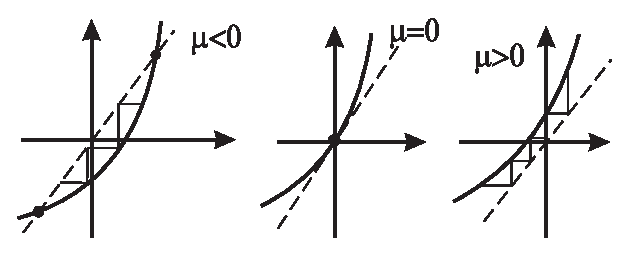
\includegraphics [scale=1.4]{jtr317}
	\caption{Bifurcation of the saddle-node for diffeomorphisms.}
	\label{fig:3.17}
\end{figure}
We also assume that for $\mu =0$ the orbit is non-hyperbolic, i.e. the constant point $z=0$ of the diffeomorphism $f_{0}$ is non-hyperbolic. Depending on the type of hyperbolic we have different types of bifurcations. We will discuss only two here.
\begin{enumerate}
	\item [\textbf{A.}]\textbf{Saddle-node bifurcation for a limit cycle.} Here we have $\lambda _{1}=1$ and $\left\vert \lambda _{j}\right\vert \not=1$ $(j>1)$ for the eigenvalues of the matrix $A$. Bringing situations to the central manifold (i.e. 1-dimensional for diffeomorphism) and applying appropriate conditions of non-degeneration (i.e. $\frac{\partial
	^{2}f}{\partial z^{2}}(0;0)$, $\frac{\partial f}{\partial \mu }(0;0)$ $\not=0)$, we reduce the situation to a 1-dimensional family following the model
	$$
	f(z;\mu) = z+\mu \pm z^2.
	$$
	
	The appropriate bifurcations are shown in Figure \ref{fig:3.17}. We see that for $\mu <0$ we have two limit cycles that merge at $\mu =0$ and then disappear.
	\item [\textbf{B.}]\textbf{Period doubling bifurcation.} Here we have $\lambda _{1}=-1$ and $\left\vert \lambda _{j}\right\vert \not=1$ for $j>1.$ Because the transformation of the return map changes the orientation, the central manifold for the orbit is a Möbius strip (see Figure \ref{fig:3.19}).
	\begin{figure}[!ht]
		\centering
		\includegraphics [scale=1.4]{jtr318}
		\caption{Period doubling bifurcation for diffeomorphisms.}
		\label{fig:3.18}
	\end{figure}
	
	The model family transformed in this case is
	$$
	f_{\mu }(z)=f(z,\mu )=\left( -1+\mu \right) z\pm z^{3}.
	$$
	Of course, this transformation has only one fixed point, i.e. $z = 0$. But its second iteration has the form
	$$
	f_{\mu }\circ f_{\mu }(z)=(1-2\mu )z\mp 2z^{3}+\ldots
	$$
	and has two additional fixed points $z_{1,2}\approx \sqrt{\mp \mu }$ for $%
	\mp \mu >0$. These fixed points correspond to the periodic orbit for $f_{\mu}$ with period 2. Thus, the name of bifurcation is taken; sometimes also the name \textit{fork bifurcation} is used (from the shape of the curve of periodic points on the plane$\left( \mu ,z\right)$).
	
	The appropriate bifurcations for $\left\{ f_{\mu }\right\} $ are shown in Figure \ref{fig:3.18}.\footnote{The Period doubling bifurcation lies at the basis of the known Feigenbaum bifurcation for the irreversible transformation of the episode $g:I\longmapsto I$ into itself. First, the fixed point loses stability when passing the eigenvalue by -1. Then there is a periodic period of rotation with period 2 again loses stability and a periodic orbit of period $2^2$ is created, etc. For the parameter's limiting value, we have Feigenbaum bifurcations.}
	
	\begin{figure}[!ht]
		\centering
		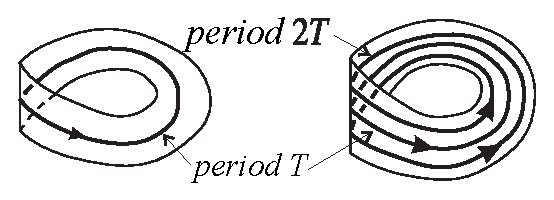
\includegraphics [scale=1.4]{jtr319}
		\caption{Period doubling bifurcation for limit cycles.}
		\label{fig:3.19}
	\end{figure}
\end{enumerate}

On this end we discuss the bifurcation of vector fields. For more details on the bifurcation described above and other bifurcations I refer the readers to literature (\cite{ALG1}, \cite{ALG2}, \cite{Ar2}, \cite{ArPl},
\cite{BaLe}, \cite{BNF}, \cite{GuHo}, \cite{MaMc}).

\chapter{Equations with a small parameter}
A small parameter in the differential equation can appear in essentially two ways:  either on the right side or on the left side. In the first case we deal with a small perturbation of the system, which we know a lot about in general and in the second case they are so-called relaxation oscillations. Both cases are discussed in successive sections.

\section{Averaging}
An example of a system from the first group is the known Van der Pole system
$$
\dot{x}=y,\text{ \ }\dot{y}=-x+\varepsilon (1-x^{2})y,
$$
where $\varepsilon$ is our small parameter. This is a special case of a perturbation of the Hamiltonian system with one degree of freedom (with the Hamiltonian function: $H(x,y)=1/2 x^2 + 1/2 y^2$)
\begin{equation}
\label{4.1}
\dot{x} = \frac{\partial H}{\partial y} +\varepsilon P(x,y),\text{ \ \ }\dot{y}%
=-\frac{\partial H}{\partial x} +\varepsilon Q(x,y).
\end{equation}
In applications often appear Hamiltonian systems with many degrees of freedom of the form 
\begin{equation}
\label{4.2}
\dot{q}_{i}= \frac{\partial H}{\partial p_i},\text{ \ \ }\dot{p}_{i}=- \frac{\partial H}{\partial q_i},%
\text{ \ \ \ }i=1,\ldots n,
\end{equation}
where $q_i$ are generalized coordinates, $p_i$ are generalized momenta and the function \linebreak
$H(q_{1}, \ldots, q_{n}, p_{1}, \ldots, p_{n})$ is a \textbf{hamiltonian function}, or \textit{Hamiltonian} (Tasks 4.11 and 4.12). In general, the system \eqref{4.2} can not be solved. However, there is a class of Hamiltonian systems fully solvable.

\begin{definition}\label{def:4.1}
	The system \eqref{4.2} is called \textbf{completely integrable} if there is a system of \textbf{functionally independent} of the first integrals $F_1 = H, F_2,\ldots , F_n$ such that each function $F_j$ is the first integral for other Hamiltonian systems generated by other $F_i$ functions. It is also said that the \textit{functions} $F_j$ \textit{are in involution}, i.e.
	$$ \sum_{i=1}^{n} \frac{\partial F_i}{\partial q_i} \dot{q_i} + \sum_{i=1}^{n} \frac{\partial F_i}{\partial p_i} \dot{p_i} = \sum_{i=1}^{n} \frac{\partial F_i}{\partial q_i} \frac{\partial F_k}{\partial p_i} + \sum_{i=1}^{n} \frac{\partial F_i}{\partial p_i} \left( -\frac{\partial F_k}{\partial q_i}\right) = 0.$$
\end{definition}

Examples of completely integrable systems are the Kepler problem and geodesic flow on the surface of an ellipsoid (see \cite{Ar3}); both have two degrees of freedom.

For systems that satisfy the condition of Definition \ref{def:4.1}, the following statement is made, which we quote without proof (see \cite{Ar3}).

\begin{theorem} \emph{(Liouville-Arnold).}\label{theo:4.4}
	If the common levels $\{F_{1}=c_{1},\ldots ,$ $F_{n}=c_{n}\}$ of a completely integrable Hamiltonian system are compact and smooth, these are the $\mathbb{T}^n$ torus.
	
	In addition, in the neighborhood of a given torus there is a system of coordinates $\left( I_{1},\ldots ,I_{n},\varphi _{1},\ldots ,\varphi
	_{n}\right) $, the so-called \textbf{action-angle variables}, in which the system \eqref{4.2} takes the following Hamiltonian form 
	\begin{equation}
	\label{4.3}
	\dot{I}_{j}=0,\text{ \ \ }\dot{\varphi}_{j}=\omega _{j}(I)=\partial
	H_{0}/\partial I_{j},\text{ \ \ \ \ }j=1,\ldots ,n,
	\end{equation}
	where $H(q,p)=H_{0}(I_{1},\ldots ,I_{n})$ is the Hamiltonian after the exchange. In general, torus movement $\left\{
	I_{1}=d_{1},\ldots ,I_{n}=d_{n}\right\} $, which are parameterized by angles $\varphi _{j}$ mod $2\pi $, is periodic or quasi-periodic (see Figure \ref{fig:4.1}):
	$$
	\varphi _{j}(t)=\varphi _{j}(0)+\omega _{j}(I)t.
	$$
\end{theorem}

\begin{figure}[!ht]
	\centering
	\includegraphics [scale=1.4]{jtr41}
	\caption{The dynamics are quasi-periodic on a torus.}
	\label{fig:4.1}
\end{figure}

\begin{example}
	For the Van der Pol system with $\varepsilon =0$ and $H=%
	\frac{1}{2}(x^{2}+y^{2})$, the action-angle variables are: $I=H$ and $\varphi =\arg (x+iy).$
	
	Consider now the following perturbation of system \eqref{4.3}
	\begin{equation}
	\label{4.4}
	\dot{I}=\varepsilon g(I,\varphi ),\text{ \ \ }\dot{\varphi}=\omega
	(I)+\varepsilon f(I,\varphi ),
	\end{equation}
	where $I=(I_{1},\ldots ,I_{n}),$ $\varphi =(\varphi _{1},\ldots ,\varphi
	_{n})$\ and $\omega =\left( \omega _{1},\ldots ,\omega _{n}\right) $.
	It is natural to expect that the solution of the system \eqref{4.4} after time of order $O(1)$ differs from the solution of the system \eqref{4.3} with the same initial conditions by size of order $O(\varepsilon )$. Meanwhile, Theorem \ref{theo:4.4} says that the same size $O(\varepsilon )$ can be obtained after a time that tends to infinity at $\varepsilon \rightarrow 0.$ This kind of phenomenon takes place thanks to the so-called averaging.
	
	The idea of averaging is connected with the fact that on the surface of torus $\mathbb{T}^{n}=\left\{ I=d\right\} $ the trajectories of a non-perturbed system are dense (as in Figure \ref{fig:4.1}). Therefore, the average deviation of action $I(t)$ can be calculated (approximately) by averaging on the torus.
\end{example}

We define the average system
\begin{equation}
\label{4.5}
\dot{J}=\varepsilon G(J),
\end{equation}
where
$$
G(J)=\left( \frac{1}{2\pi }\right) ^{n}\int_{0}^{2\pi }\ldots \int_{0}^{2\pi
}g(J,\varphi )d\varphi _{1}\ldots d\varphi _{n}
$$
is the average of the speed of change of action on $\mathbb{T}^{n}$.

\begin{theorem}\emph{(About averaging).}
	Let $n=1$ and functions $\omega ,f,g$ be of class $C^1$ and $\omega (I)>0$ be an open subset of $\mathbb{R}^{1}\times \mathbb{T}^{1}$. If $\left( I(t),\varphi (t)\right) $ and $\left( J(t),\psi (t)\right) $ are solutions of the systems \eqref{4.4} and \eqref{4.5} such that $I(0)=J(0)$, then for
	$$
	0<t<1/\varepsilon
	$$
	we have
	$$
	\left\vert I(t)-J(t)\right\vert <C\cdot \varepsilon ,
	$$
	where constant $C$ depends only on $\omega ,f,g.$
	\begin{proof}
		Let's replace
		\begin{equation}
		\label{4.6}
		K=I+\varepsilon k(I,\varphi )
		\end{equation}
		so that there is $\dot{K}=O(\varepsilon ^{2})$. The calculation $k(J,\varphi
		)$ follows form the following
		$$
		\begin{array}{lll}
		\dot{K} &=&\dot{I}+\varepsilon \frac{\partial k}{\partial I}\dot{I}%
		+\varepsilon \frac{\partial k}{\partial \varphi }\dot{\varphi}=\varepsilon
		\left\{ g+\frac{\partial k}{\partial \varphi }\omega \right\} +O(\varepsilon
		^{2}) \\
		&=&\varepsilon \left\{ g(K,\varphi )+\frac{\partial k}{\partial \varphi }%
		(K,\varphi )\omega (K)\right\} +O(\varepsilon ^{2}).
		\end{array}
		$$
		So we want to solve the equation
		$$
		\frac{\partial k}{\partial \varphi }(K,\varphi )\omega (K)=-g(K,\varphi),
		$$
		with the obvious solution $g(K,\varphi )=\frac{-1}{\omega (K)}%
		\int_{0}^{\varphi }g(K,\psi )d\psi .$  Unfortunately, usually this solution is not an explicit (or periodic) function from $\varphi$. The obstacle is the quantity $\int_{0}^{2\pi }g(h,\psi )d\psi$, which can be non-zero.
		
		But, by writing
		$$
		g(K,\varphi )=G(K)+\tilde{g}(K,\varphi )
		$$
		so that $\int_{0}^{2\pi }\tilde{g}(h,\psi )d\psi =0$, we can define the unambiguous functions
		$$
		g(K,\varphi )=\frac{-1}{\omega (K)}\int_{0}^{\varphi }\tilde{g}(K,\psi)d\psi .
		$$
		We get the equation
		$$
		\dot{K}=\varepsilon G(K)+O(\varepsilon ^{2}).
		$$
		
		You can see that after the time $O(1/\varepsilon )$ the difference between $J(t)$ and $K(t)$ is of order $O(\varepsilon )$. On the other hand, the difference between $K (t)$ and $I (t)$ is of order $O(\varepsilon )$, thanks to the change \eqref{4.6}.
	\end{proof}
\end{theorem}

For perturbations of type \eqref{4.4} of completely integral Hamiltonian systems with many degrees of freedom of estimation, they are weaker than in the thesis of Theorem \ref{theo:4.4}. It turns out that after time of order $O(1/\varepsilon ^{a})$, for initial conditions outside the set with Lebesque's measure $O(\varepsilon ^{b})$, the deviation $J(t)$ from $I(t)$ does not exceed $O(\varepsilon ^{c})$, where $a, b, c> 0$ are exponents dependent on $\omega ,f,g.$ For more information, I refer the reader to \cite{Ar2}.

\begin{example}\label{example:4.5}
	(Abel integrals). Let's consider the following perturbation of the two-dimensional Hamiltonian system
	$$
	\dot{x}=H_{x}^{\prime }+\varepsilon P(x,y),\text{ \ \ \ }\dot{y}%
	=-H_{x}^{\prime }+\varepsilon Q(x,y).
	$$
	For $\varepsilon =0$, the phase curves lie in the levels of Hamilton function $H (x, y)$. In some area of the phase space these curves are closed.
	As we have already done several times, the study of limit cycles of the perturbed system consists in analyzing the transformation of Poincaré's return from $S$ (transversal cut to phase curves) to $S$. Parameterizing $S$ with $H|_{S}$ the boundary cycle condition is $\Delta H=H(B)-H(A)=0$ (see Figure \ref{fig:4.2}). We have
	$$
	\begin{array}{lll}
	\Delta H &=&\int_{0}^{T}\frac{dH}{dt}dt=\int_{0}^{T}\left\{ H_{x}^{\prime
	}\left( H_{y}^{\prime }+\varepsilon P\right) +H_{y}^{\prime }(-H_{x}^{\prime
	}+\varepsilon Q\right\} dt \\
	&=&\varepsilon \int \left( PH^{\prime }x+QH_{y}^{\prime }\right)
	dt=\varepsilon \int \left\{ P(H_{x}^{\prime }-\varepsilon Q)+Q\left(
	H_{y}^{\prime }+\varepsilon P\right) \right\} \\
	&=&\varepsilon \int_{\Gamma (h)}Qdx-Pdy=\varepsilon \oint_{H=h}\left(
	Qdx-Pdy\right) +O(\varepsilon ^{2}),
	\end{array}
	$$
	where $T$ is the time to return to $S$ and $\Gamma (h)$ is the phase curve of the perturbed system starting from $A\in S$ such that $H (A) = h$.
	\begin{figure}[!ht]
		\centering
		\includegraphics [scale=1.4]{jtr42}
		\caption{Conversion of a return map to the perturbed Hamiltonian system.}
		\label{fig:4.2}
	\end{figure}

	The expression
	\begin{equation}
	\label{4.7}
	I(h)=\oint_{H=h}Qdx-Pdy
	\end{equation}
	is so-called \textbf{Abel's integral}.\footnote{The concept of the abelian integral derives from the complex algebraic geometry. They are integrals of meromorphic 1-forms along certain closed curves on complex algebraic curves (Riemann surfaces). When $H(x,y),$ $P(x,y)$ and $Q(x,y)$ are polynomials, then the Riemann surface is the complex curve $\left\{ H(x,y)=h\right\} \subset \mathbb{C}^{2}$ and the 1-form is $\omega = \left( Qdx-Pdy\right) |_{H=h}.$} Theorems about implicit functions result from the fact that if $I(h_{0})=0$ and $I^{\prime }(h_{0})\not=0$, then for small $\varepsilon \not=0$ and small there is a limit cycle $\gamma_{\varepsilon }$, which strokes the curve $H=h_{0}$ as $\varepsilon \rightarrow 0$. This approach to the problem of limit cycles is widely used in the Qualitative Theory.

	It is not difficult to notice that the function $I(h)$ is the equivalent of the integral of $G(J)$, which occurs in the formula \eqref{4.5}.
\end{example}

\section{KAM Theory}
Consider the Hamiltonian system
$$
\dot{q}=H_{p}^{\prime },\text{ \ \ \ }\dot{p}=-H_{q}^{\prime },
$$
$p=\left( p_{1},\ldots ,p_{n}\right) ,$ $q=\left( q_{1},\ldots ,q_{n}\right)$, with the Hamiltonian form
$$
H(p,q)=H_{0}(p,q)+\varepsilon H_{1}(p,q),
$$
where $H_{0}$ is the Hamiltonian of a completely integer system, i.e. a system of type \eqref{4.3} in action-angle variables. This situation is connected with one of the most important mathematical theorems of the second half of the XX century. Before formulating it, we have to introduce two more assumptions regarding the non-degeneration of the unperturbed $H_0$ Hamiltonian:
\begin{equation}
\label{4.8}
\det \left( \frac{\partial \omega _{i}}{\partial I_{j}}\right) =\det \left(
\frac{\partial ^{2}H_{0}}{\partial I_{i}\partial I_{j}}\right) \not=0,
\end{equation}%
\begin{equation}
\label{4.9}
\det 
\begin{pmatrix}
\frac{\partial ^{2}H_{0}}{\partial I_{i}\partial I_{j}} & \frac{\partial
	H_{0}}{\partial I_{i}} \\
\frac{\partial H_{0}}{\partial I_{j}} & 0%
\end{pmatrix} \neq 0.
\end{equation}

The condition \eqref{4.8} means that frequencies $\omega _{i}(I)$ will become independent and fit quickly with the change of actions $I_{j}$, while the condition \eqref{4.9} means that these frequencies change quickly and independently, after limitation to the levels $\left\{ H_{0}=\textrm{const}\right\}$.

\begin{theorem}\emph{(Kolmogorov–Arnold–Moser).}
	If the non-degeneration conditions \eqref{4.8} and \eqref{4.9} are satisfied for $H_{0}$, then for a small perturbation $H=H_{0}+\varepsilon H_{1}$ most of the invariant torus ${I = \textrm{const}}$ do not disappear, but only slightly deforms and movement on them are still quasi-periodic.
\end{theorem}

This theorem was formulated in 1954 at the International Congress of Mathematicians in Amsterdam, but it had to wait for the strict proof until the beginning of the sixties. It was given by V. Arnold (in the analytical case) and J. Moser (in the case of a smooth of class $C^{333}$). The smoothness class was later reduced to $C^3$. Of course I am not able to present this proof here.

\begin{example} (The flat limited problem of three bodies).
	The \textbf{flat limited problem of the three bodies} is a system in which two bodies (interacting forces of gravity) rotate at a constant angular velocity around their center of mass (at the beginning of the coordinate system) and the third body moves in the plane of rotation of two bodies and has a mass so small that it does not interfere with their movement. In Figure \ref{fig:4.3} we have a system in which $S$ means Sun, $J$ means Jupiter, and $A$ is an Asteroid. Units of time, length and mass can be chosen so that the angular velocity, the sum of  the masses of $S$ and $J$ and the gravitational constant are equal to 1. Then the distance between $S$ and $J$ also equals 1. The only parameter characterizing the system is the mass of Jupiter $\mu$.
	
	The Asteroid motion equations are Hamiltonian with the Hamiltonian
	$$
	\frac{1}{2}(p_{1}^{2}+p_{2}^{2})-\frac{1-\mu }{\rho _{1}}-\frac{\mu }{\rho_{2}},
	$$
	where $\rho _{1}$ and $\rho _{2}$ are the distances $A$ from $S$ and $J$, respectively. Note that the positions $S$ and $J$ change over time: $J=\left( 1-\mu \right) (\cos t,\sin t),$\ $S=(-\mu
	)\left( \cos t,\sin t\right)$; therefore, the Hamiltonian depends directly on time.
	\begin{figure}[!ht]
		\centering
		\includegraphics [scale=1.4]{jtr43}
		\caption{The problem of three bodies and invariant torus.}
		\label{fig:4.3}
	\end{figure}

	To get rid of this dependence on time, we make the following change (simultaneous rotation of coordinates and sprouts)
	$$
	q^{\prime }=M(t)q,\text{ \ \ }p^{\prime }=M(t)p,\text{ \ \ }M(t)=\left(
	\begin{array}{ll}
	\cos t & \sin t \\
	-\sin t & \cos t%
	\end{array}%
	\right) .
	$$
	It turns out that the new variables are still Hamiltonian with the new Hamiltonian
	\begin{equation}
	\label{4.10}
	H =\frac{1}{2}\left( p_{1}^{\prime }+q_{2}^{\prime }\right) ^{2}+\frac{1}{2%
	}\left( p_{2}^{\prime }-q_{1}^{\prime }\right) ^{2}-V(q_{1}^{\prime
	},q_{2}^{\prime }),
	\end{equation}
	
	$$
	V =\frac{q_{1}^{\prime 2}+q_{2}^{\prime 2}}{2}+\frac{1-\mu }{\rho _{1}}+%
	\frac{\mu }{\rho _{2}},
	$$
	$\rho _{1}^{2}=\left( q_{1}^{\prime }+\mu \right) ^{2}+q_{2}^{\prime 2}$, $\rho _{2}^{2}=\left( q_{1}^{\prime }+\mu -1\right) ^{2}+q_{2}^{\prime 2}$ (Task 4.13). In the new variables $q_{1}^{\prime }$, $q_{2}^{\prime }$, the bodies $S$ and $J$ are resting.
	
	The Hamiltonian's system equilibrium points are the critical points of the Hamiltonian function (Task 4.14). In the case of Hamiltonian \eqref{4.10}, these points, which we call \emph{relative positions of equilibrium}, are given by 
	$$
	p_{1}^{\prime }=-q_{2}^{\prime },\text{ \ \ }p_{2}^{\prime }=q_{1}^{\prime },%
	\text{ \ \ }\partial V/\partial q_{1}^{\prime }=\partial V/\partial
	q_{2}^{\prime }=0.
	$$
	We have
	\begin{eqnarray*}
		\frac{\partial V}{\partial q_{2}^{\prime }} &=&q_{2}^{\prime }\left( 1-\frac{%
			1-\mu }{\rho _{1}^{3}}-\frac{\mu }{\rho _{2}^{3}}\right) =q_{2}^{\prime }f,
		\\
		\frac{\partial V}{\partial q_{2}^{\prime }} &=&q_{1}^{\prime }f-\mu (1-\mu
		)\left( \frac{1}{\rho _{1}^{3}}-\frac{1}{\rho _{2}^{3}}\right) .
	\end{eqnarray*}
	We have two options:
	\begin{enumerate}
		\item $q_{2}^{\prime }=0$; here we find three points of the so-called \emph{collinear liberty points} $L_{1}$, $L_{2}$, $L_{3}$	(Task 4.15), which are unstable.
		\item $f=0$ and $\rho _{1}=\rho _{2}=1$; here we have two so-called \emph{triangular points of liberty} $L_4$ and $L_5$, which lies in the vertices of two equilateral triangles with a base $\overline{SJ}.$
	\end{enumerate}

	Calculations that we do not carry out show that for $27\mu
	(1-\mu )>1$, $L_{4,5}$ points are unstable whereas in the opposite case, i.e. for $\mu <\mu _{1}=\frac{1}{2}(1-\sqrt{23/27})\approx 0.03852$, the eigenvalues of the linear part of the Hamiltonian system are in the form $\pm i\omega _{1}$, $\pm i\omega _{2}$, where $\omega _{1}<0<\omega _{2}\not=\omega _{1}$. We are on the border of the stability area.
	
	In addition, the square part of $H$ at point $L_{4}$ takes the form
	$$
	H_{0}=\frac{1}{2}\omega _{1}(\tilde{p}_{1}^{2}+\tilde{q}_{1}^{2})+\frac{1}{2}%
	\omega _{2}\left( \tilde{p}_{2}^{2}+\tilde{q}_{2}^{2}\right)
	$$
	in the appropriate coordinate system in the neighborhood of $L_{4}$ (see \cite{Zol1}). It is a completely integrable Hamiltonian system with a change in action-angle $I_{1}=\frac{1}{2}(\tilde{p}_{1}^{2}+\tilde{q}%
	_{1}^{2})$, $I_{2}=\frac{1}{2}\left( \tilde{p}_{2}^{2}+\tilde{q}%
	_{2}^{2}\right) $, $\varphi _{1}=\arg \left( \tilde{q}_{1}+i\tilde{p}%
	_{1}\right) $, $\varphi _{2}=\arg \left( \tilde{q}_{2}+i\tilde{p}%
	_{2}\right) $ and with $H_{0}=\omega _{1}I_{1}+\omega _{2}I_{2}$ (Task 4.16).
	
	We have situations like in KAM theorem: $H=H_{0}+H_{1}$, where $H_0$ is completely integrable and $H_1$ contains terms of order $> 2$ due to $I_{j}$ (which are small). Unfortunately, this is not enough because the frequencies of $\omega _{j}=\partial H_{0}/\partial I_{j}$ are constant, and from the condition of non-degeneration \eqref{4.8} should change with $I_{j}$. Therefore, we should take into account further terms of the $H$ expansion in the $L_4$ neighborhood.
	
	More specifically, we simplify the terms of the third and fourth order in the Hamiltonian $H$. This simplification is an analogue of Poincaré-Dulac's normal form and has been proved by G. Birkhoff in Theorem \ref{theo:4.9} below. This \emph{Birkhoff normal form} in our case has the following form
	\begin{equation}
	\label{4.11}
	H=H_{0}+H_{1},\text{ \ }H_{0}=\omega _{1}I_{1}+\omega _{2}I_{2}+\sum \omega
	_{ij}I_{i}I_{j},\text{ \ }I_{j}=\frac{1}{2}(P_{j}^{2}+Q_{j}^{2}),
	\end{equation}
	where $P_{j}=\tilde{p}_{j}+\ldots$, $Q_{j}=\tilde{q}_{j}+\ldots $ are new variables and $H_1$ contains terms of order 5 (and $H_0$ and $H_1$ are different than above). In the assumption of Birkhoff's theorem, there is a condition of no resonant relations of order 4 and 3. It turns out that such relations occur for the values of $\mu_{2}=\frac{1}{2}\left( 1-\sqrt{1833}/45\right) \approx 0.02429$ and $\mu _{3}=\frac{1}{2}\left( 1-\sqrt{213}/15\right) \approx 0.01352$; therefore, these values of the $\mu$ parameter should be excluded.
	
	Hamiltonian $H_{0}=H_{0}(I_{1},I_{2})$ is a completely integrable Hamiltonian and has a chance of satisfying non-degeneration conditions \eqref{4.8} and \eqref{4.9}. It turns out that only condition \eqref{4.9} is significant. A. Leontovych showed that it can be violated only for a discrete set of values of parameter $\mu$.\footnote{In \cite{Zol1} one can find out that the condition \eqref{4.9} is violated for adding one specific value of the $\mu$ parameter. This value resulted from the formula for the determinant in equation \eqref{4.9} given by the French astronomers A. Deprit and A. Deprit-Bartholomé (and cited in very serious monographs). Recently, with my graduate student W. Barwicz, we discovered that this pattern is not true, and even contrary to the calculations of Leontovych. In fact, the determinant is a very complicated algebraic function from $\mu$, which is not identical to zero.} Let us assume then that $\mu$ satisfies all the conditions listed above, which is the real thesis of KAM theorem.
	
	How does stability result from the KAM theorem? Well, we are in a 4-dimensional space surrounded by an equilibrium point. Because the system is Hamiltonian with the Hamiltonian independent of time, so the movement takes place on the surfaces $H=\textrm{const}$. They are three-dimensional. From the KAM theorem, it follows that every such surface is almost filled with the invariant torus $\mathbb{T}^{2}$, which is the more we are closer to the torus $I_{1}=I_{2}=0$. Each invariant torus breaks down the $H=\textrm{const}$ surface into two parts, its interior and exterior. No interior point comes out of it during evolution. Because in the space of P, Q variables, toruses can be arbitrarily small, this results in stability in the sense of Lyapunov.
\end{example}

We will complete the above example. Let's assume we have a Hamiltonian in the form
$$
H=\sum \omega _{j}\cdot \frac{1}{2}(p_{j}^{2}+q_{j}^{2}) + \ldots .
$$

\begin{definition}
	We say that the `frequencies' $\omega _{j}$ satisfies the \textbf{resonance relations of order} $d$, if there are integers $k_{1},\ldots ,k_{n}$ with $\sum \left\vert
	k_{j}\right\vert =d$ such that
	$$
	\sum k_{j}\omega _{j}=0.
	$$
\end{definition}

\begin{theorem}\label{theo:4.9}\emph{(Birkhoff).}
	If the frequencies $\omega _{j}$ do not satisfy any resonant relation of order $\leq 2m$, then there is a canonical exchange of variables $\left( p,q\right) \longmapsto \left( P,Q\right) =\left( p+\ldots ,q+\ldots
	\right) $ leading to the Hamiltonian
	$$
	H=\sum_{\left\vert l\right\vert \leq m}a_{l}I^{l}+O\left( \left\vert \left(
	p,q\right) \right\vert ^{2m+1}\right) ,
	$$
	where $I_{j}=\frac{1}{2}(P_{j}^{2}+Q_{j}^{2})$ and the summation runs along the $\left( l_{1},\ldots
	,l_{n}\right) $ multi-planes with $\left\vert l\right\vert =l_{1}+\ldots +l_{n}$ and $I^{l}=I_{1}^{l_{1}}\ldots I_{n}^{l_{n}}$.
\end{theorem}

\begin{remark}
	Conversion $\left( p,q\right) \longmapsto \left(P,Q\right) $, occurring in the above theorem is canonical if
	$$
	\sum dp_{j}\wedge dq_{j}=\sum dP_{j}\wedge dQ_{j}.
	$$
	It turns out that after the canonical exchange of variables, the Hamiltonian system changes into the Hamiltonian system (see \cite{Ar3}).
\end{remark}

\subsection*{Tasks}
\begin{task}
	Show that if the Hamilton function $H$ does not depend directly on time, it is the first integral for the system \eqref{4.2}.
\end{task}

\begin{task}
	Show that the vector field given by the formula \eqref{4.2} has zero divergence. Deduce the form that the corresponding phase stream keeps its volume.
\end{task}

\begin{task}
	Prove formula \eqref{4.10}.
\end{task}

\begin{task}
	Show that if $H$ does not depend directly on time, the equilibrium points of the system \eqref{4.2} are exactly critical points of the function $H$.
\end{task}

\begin{task}
	Show that there are exactly three collinear libration points.
\end{task}

\begin{task}
	Show that the Hamiltonian form $H_{0}=\omega
	_{1}I_{1}+\omega _{2}I_{2}$ (or as in formula \eqref{4.11}) is the Hamiltonian of a completely integrable system.
\end{task}

\begin{task}
	Apply the abelian integrals method (Example \ref{example:4.5}) to show that the van der Pol system $\dot{x}=y$, $\dot{y} = -x-a(x^{2}-1)y$ for the small parameter $a> 0$ has exactly one boundary cycle.
\end{task}

\section{Relaxation oscillations (slow-fast systems)}
Let's start with a known example.
\begin{example}(Van der Pol system).
	$$
	\dot{x}=y-x^{3}+x,\text{ \ \ }\dot{y}=-\varepsilon x.
	$$
	(When $\varepsilon =1$ and place $y_{1}=y-x^{3}+x$, then it gets $\dot{x}=y_{1}$, $\dot{y}_{1}=-x-(3x^{2}-1)y_{1}$; exact to scale it is the system from Example \ref{example:2.35}
	\begin{figure}[!ht]
		\centering
		\includegraphics [scale=1.4]{jtr44}
		\caption{The Van der Pol system	`slow-fast' type.}
		\label{fig:4.4}
	\end{figure}
	
	You can see that $x$ changes quickly compared to $y$; we say that $x$ is a \emph{fast variable} and $y$ is \emph{slow}. For $\varepsilon =0$ we have $y = \textrm{const}$ and in fact we have the equation for $x$ dependent on the parameter $y$	(theory of bifurcation bows, see Figure \ref{fig:4.4}). When $\varepsilon \not=0$ (but small), physicists would say that the parameter $y$ `flows'. It is expected that there will be a limit cycle $\gamma _{\varepsilon }$ (in fact $\gamma _{\varepsilon }$ is stable) to the slices of the smooth curve $\gamma_0$ shown in Figure \ref{fig:4.5}. The $\gamma _0$ cycle consists of:
	\begin{itemize}
		\item pieces of slow motion along the curve $y=x^{3}-x$ (where $\dot{x}=0$),
		\item sections of a jump along the straight $y = \textrm{const}$.
	\end{itemize}

	Such movement is an example of relaxation oscillations (like a heartbeat).
	\begin{figure}[!ht]
		\centering
		\includegraphics [scale=1.4]{jtr45}
		\caption{Relaxation oscillations.}
		\label{fig:4.5}
	\end{figure}
\end{example}

Consider now the general situation. We have an \textbf{unperturbed system}
$$
\dot{x}=f(x,y),\text{ \ \ \ }\dot{y}=0,
$$%
($x\in \mathbb{R}^{k}$, $y\in \mathbb{R}^{l}$); here $x$ are the \textbf{fast coordinates} and $y$ are the \textbf{slow coordinates}. We also have the \textbf{perturbed system}
$$
\dot{x}=F(x,y;\varepsilon ),\text{ \ \ }\dot{y}=\varepsilon
G(x,y;\varepsilon ),\text{ \ \ \ }F(x,y;0)=f(x,y).
$$

\begin{definition}
	The surface $S = {f (x, y) = 0}$ is called  \textbf{slow surface}.
	
	The slow surface is divided into \textbf{areas of stability} and \textbf{instability} of the undisturbed system; they correspond to situations when $\textrm{Re}\lambda _{j}(A)<0$, $j=1,\ldots ,k$, $A=\frac{\partial f}{\partial x}$, and when there is $\textrm{Re}\lambda _{j}(A)>0$.
	
	On a slow surface, we have a vector field defined as follows. We take the field
	$$
	\frac{\partial }{\partial \varepsilon }\left( F\partial _{x}+\varepsilon
	G\partial _{y}\right) |_{\varepsilon =0}=f_{1}(x,y)\partial
	_{x}+g(x,y)\partial _{y}
	$$
	at point $\left( x,y\right) \in S$ and project it on $T_{(x,y)}S$ along the variable $y$. This is a \textbf{slow motion field}.
\end{definition}

Let us reminding that at the beginning of this chapter we were saying that relaxation oscillations are characterized by the fact that a small parameter appears on the left side. To find out, we introduce slow time $\tau =\varepsilon t$. Then we get the system
$$
\varepsilon \frac{dx}{d\tau }=f(x,y)+O(\varepsilon ),\text{ \ \ }\frac{dy}{%
	d\tau }=g(x,y)+O(\varepsilon ).
$$
Now the \emph{slow motion equation} to $S$ (locally parameterized by $y$) has the form
$$
\frac{dy}{d\tau }=h(y)+O(\varepsilon )
$$
(with the corresponding function $ h$).

Let's analyze the movement of a typical point $(x_0, y_0)$. It consists of pieces of three types: approaching to the slow surface, movement along the slow surface and movement in the transition area.

\begin{figure}[!ht]
	\centering
	\includegraphics [scale=1.4]{jtr46}
	\caption{Approaching to the slow surface.}
	\label{fig:4.6}
\end{figure}

\subsection{Approaching to the slow surface}
Let the point $(x_0, y_0)$ from outside $S$ be projected (along the $y$ coordinates) to the point $(x_*, y_0)$, $x_* = x_* (y_0)$, to $S$ in the stability area (see Figure \ref{fig:4.6}). This means that point $x_0$ lies in the pool of attraction of the point $x_*$ for the equation $\dot{x} = f (x, y_0)$ ($y_0$ fixed). Consider the area $U = {\left| x - x_* (y_0) \right| <\delta, y_0 \in V}$, where $V$ is a certain area corresponding to a subset of the stability area in $S$. It turns out that the slow recovery time of the solution with the initial condition $(x_0, y_0)$ to $U$ is of order $\tau_1 \sim C_1 \varepsilon \left|\ln \varepsilon\right|$, which corresponds to the actual time
$$
t_1 \sim C_1  \left|\ln \varepsilon\right|
$$
$$
r(t)<C_{1}e^{-C_{2}/\varepsilon }\rightarrow 0,
$$
(constant $C_1$ depends on $U$ and $F$, $G$).

\subsection{Movement along the slow surface}
In the area of $U$, we have slow motion, described by the equation $dy/d\tau =h(y)+O(\varepsilon )$. It lasts until $\tau_{2}=T=O(1)$, which corresponds to the long real time $t_{2}=T/\varepsilon .$

\subsection{Movement in the transition area}
The transition area lies close to the border between the areas of stability and instability in $S$. We have two typical options (as in the bifurcation theory):
\begin{enumerate}
	\item[\textbf{A.}] $\lambda_1(A) = 0$ (where $A = \frac{\partial f}{\partial x} \mid_{f = 0})$;
	\item[\textbf{B.}] $\Re \lambda_{1,2} =0$.
\end{enumerate}

\subsubsection{A. Spurt}
This case (which corresponds to saddle-node bifurcation) is analyzed for situations where $x \in \mathbb{R}$ and $y \in \mathbb{R}$ (you can reduce everything to this). After the appropriate rescaling, we have the following system
$$
\dot{x}=x^{2}-y+\ldots ,\text{ \ \ }\dot{y}=-\varepsilon +\ldots
$$
We normalize
$$
\varepsilon =\mu ^{3},\text{ \ \ }x=\mu X,\text{ \ \ }y=\mu^{2}Y.
$$
and it is easy to check that it leads to the field
$$
\dot{X}=\mu \left\{ X^{2}-Y+O(\mu )\right\} ,\text{ \ \ }\dot{Y}=\mu \left\{-1+O(\mu )\right\}
$$
orbitally equivalent to field $\left( X^{2}-Y\right) \partial_{X}-\partial _{Y}$. Its phase portrait is given by the Riccati equation
\begin{equation}
\label{4.12}
dX/dY=Y-X^{2}
\end{equation}
and is shown in Figure \ref{fig:4.7}.\footnote{The equation \eqref{4.12} is probably the simplest example of a differential equation that can not be solved in the so-called quadrature.} The phenomenon that we observe here is called the \textbf{spurt}.

\begin{figure}[!ht]
	\centering
	\includegraphics [scale=1.4]{jtr47}
	\caption{The phenomenon of `spurt'.}
	\label{fig:4.7}
\end{figure}

\subsubsection{B. Delay in the loss of stability.}
In this case, which corresponds to the Andronov-Hopf bifurcation, the problem is reduced to the following model system
\begin{equation}
\label{4.13}
\dot{z}=\left( y+i\omega \right) z+cz\left\vert z\right\vert ^{2},\text{ \ \
}\dot{y}=\varepsilon ,
\end{equation}
$z = x_{1}+ix_{2}\in \mathbb{C}\simeq \mathbb{R}^{2},$ $y\in \mathbb{R}.$ Of course, $y=\varepsilon t$ is a `flowing' parameter. Suppose further that
$$
c=-1;
$$
the case of $c> 0$ is less interesting. For the amplitude $r=\left\vert z\right\vert$ we get the Bernoulli equation
$$
\dot{r}=r\left( \varepsilon t-r^{2}\right).
$$

Let's put the initial condition
$$
y(t_{0})=-\mu ,\text{ \ \ \ }r(t_{0})=r_{0},\text{ \ \ }t_{0}=-\mu
/\varepsilon ,
$$
where $\mu >0$ is a fixed constant (not too big and not too small). This initial problem has the following solution
\begin{equation}
\label{4.14}
r(t)=r_{0}\left\{ e^{\varepsilon \left( t_{0}^{2}-t^{2}\right)
}+2r_{0}^{2}\int_{t_{0}}^{t}e^{\varepsilon \left( s^{2}-t^{2}\right)
}ds\right\} ^{-1/2}
\end{equation}
(Task 4.24). We will examine the asymptotic behavior of this solution at $\varepsilon \to 0$ by dividing the time range $t$ into four areas:
\begin{enumerate}[(a)]
	\item $0<t-t_{0}<O(1)$, or $0<y+\mu <O(\varepsilon ).$\\
	Let $u=t-t_{0}$. Then $\varepsilon \left( t_{0}^{2}-t^{2}\right)
	=\varepsilon (t_{0}+t)u\approx 2\mu u$ and $\varepsilon \left(
	s^{2}-t^{2}\right) \approx 2\mu (u-v)$, where $v=s-t_{0}$. Thus,
	$$
	\int_{t_{0}}^{t}e^{\varepsilon \left( s^{2}-t^{2}\right) }ds\approx
	\int_{0}^{u}e^{2\mu (u-v)}dv=\frac{1}{2\mu }(e^{2\mu u}-1)
	$$
	and
	$$
	r(t)\approx r_{0}\left\{ e^{2\mu u}+r_{0}^{2}(e^{2\mu u}-1)/\mu \right\}
	^{-1/2}
	$$
	is a decreasing function from $u$.
	\item $y=\varepsilon t$ is the set such that $-\mu <y<\mu$.\\
	Here, $e^{\varepsilon \left( t_{0}^{2}-t^{2}\right) }\approx e^{\left( \mu
		^{2}-y^{2}\right) /\varepsilon }\rightarrow \infty$. Thus,
	$$
	r(t)<C_{1}e^{-C_{2}/\varepsilon }\rightarrow 0,
	$$%
	which is a very quick pursuit of zero.
	\item $0<\left\vert t_{0}\right\vert -t<O(1)$, or $0<\mu -y<O(\varepsilon )$\\
	Let's introduce the variable $w=\left\vert t_{0}\right\vert -t$. As in case (a), we have $e^{\varepsilon \left( t_{0}^{2}-t^{2}\right) }\approx
	e^{2\mu w}.$
	
	We will divide the integration area for the integral in the formula \eqref{4.14} into three sections: from $t_{0}$ to $t_{0}/2<0$, from $t_{0}/2$ to $\left\vert t_{0}\right\vert /2$ and from $\left\vert t_{0}\right\vert /2$ to $t$. Through $I_{1},$ $I_{2}$ and $I_{3}$ we will determine the relevant integrals. Similarly as in case (a), it shows that $I_{1}=O(1)$ and $I_{3}=O(1)$. The calculations in (b) show that $I_{2}\to 0$ very quickly. Thus,
	$$
	r(t)=O(1).
	$$
	\item $\left\vert t_{0}\right\vert <t$, or $y>\mu $ and it is fixed. Now
	$e^{\left\{ \varepsilon \left( t_{0}^{2}-t^{2}\right) \right\}} \approx e^{\left\{ -(y^{2}-\mu ^{2})/\varepsilon \right\}} \to 0$. Then $\varepsilon \left( s^{2}-t^{2}\right) \approx (s-t)\cdot 2y$ for $s$ close to $t$, i.e. for those $s$, for which the contribution to the integral is dominant. We get $\int^{t}e^{2y(s-t)}ds \approx \frac{1}{2y}$. Hence
	$$
	r(t)\approx r_{0}\left\{ r_{0}^{2}/2y\right\} ^{-1/2}=\sqrt{y}.
	$$
\end{enumerate}

\begin{figure}[!ht]
	\centering
	\includegraphics [scale=1.4]{jtr48}
	\caption{The phenomenon of delayed loss of stability.}
	\label{fig:4.8}
\end{figure}

We can summarize the above calculation.

\begin{theorem}
	In the case B described by the system \eqref{4.13} with $c <0$, the phenomenon of delay in the loss of stability occurs. It depends on changing the variable $y$ (which is the coefficient of unstable motion of stability) from the negative value $y(t_{0})=-\mu $ to the positive value $\mu $ the system (with respect to $z$) is stable all the time, and the change in the stability of the solution takes place for parameter $y = \mu $, whereby the amplitude of the oscillation increases as in the normal Andronov-Hopf bifurcation.
\end{theorem}

The phenomenon of \textbf{delay in the loss of stability} can be explained physically. The variable $y$ is negative for a very long time, on the order of $1/\varepsilon$. Then the physical system will come very close to the balance; close enough that you need the same amount of time later to leave the balance (see Figure \ref{fig:4.8}).


\subsection*{Tasks}
\begin{task}
	Prove formula \eqref{4.14}.
\end{task}

\chapter{Chaotic dynamics in differential equations}
\section{Introduction to chaos theory and one example}

For the autonomous vector field in $\mathbb{R}^{2}$ the phase portrait and movement is fully determined; this is described in Section \ref{2.4}. But when the phase space is not so simple, interesting phenomena can happen.

\begin{figure}[!ht]
	\centering
	\includegraphics [scale=1.5]{jtr51}
	\caption{Transitivity and mixing.}
	\label{fig:5.1}
\end{figure}

For example, a fixed vector field
$$
\dot{\varphi}_{1}=\omega _{1},\dot{\varphi}_{2}=\omega _{2}
$$
on the torus $\mathbb{T}^{2}=\left\{ \left( \varphi _{1}, \varphi_{2}\right) \right\} $ can have dense phase curves, i.e. when $omega_{2}/\omega _{1}$ is irrational. Then the phase curves are dense (as in Figure \ref{fig:4.1} above) and the motion is \emph{quasi-periodic}, which means that the solution returns roughly periodically to each small area of the phase space. In addition, you can reach any other small area from any small area. Such property is called \emph{transitivity} in the theory of Dynamic Systems. The movement is not fully deterministic, because after a long time it is difficult to say where the evolving particle is. However, this is not a chaotic movement, because if at the beginning we had a focused area of the phase space, then this area retains its focused shape during evolution. Meanwhile, in a \emph{chaotic movement}, such a cell begins to `dissolve' in the phase space.

\begin{example} (Transitivity and chaos).
	A good example of a situation illustrating the difference between transitivity and chaos are two glasses of water, such that one dropped in a small drop of oil and the other one poured the same amount of juice (Figure \ref{fig:5.1}). The oil droplet will drift, visit every spot in the water, and the juice will start to dissolve, filling the entire water area evenly (this property is also called \emph{mixing}).
\end{example}

\begin{figure}[!ht]
	\centering
	\includegraphics [scale=1.5]{jtr52}
	\caption{Swing.}
	\label{fig:5.2}
\end{figure}

Perhaps the simplest differential systems in which chaos can be observed are periodic non-autonomous systems of the form
\begin{equation}
\label{5.1}
\dot{x}=v(t,x),\text{ \ \ }x\in M,\text{ \ \ }v(t+T,x)=v(t,x),
\end{equation}
where $M$ is a $2-$dimensional variety. As we know, such a system can be treated as autonomous in the expanded phase space $\mathbb{S}^{1}\times M$. Then it is convenient to work with the monodromy map (after the period)
$$
\mathcal{P}:M\longmapsto M,\text{ \ \ \ } \mathcal{P}=g_{0}^{T},
$$
where $g_{s}^{t} = \phi(t; x_0, s)$, $\phi(s;x_0, s) = x_0$, is a $2-$parameter family of diffeomorphisms defining evolution. In terms of the extended phase space it is the conversion of the return map to the hypersurface $\left\{0\right\} \times M$. In the monograph of J. Guckenheimer and P. Holmes \cite{GuHo}, an example of the Duffing system is analyzed with the external force
$$
\ddot{x}=x-x^{3}+\varepsilon \left\{ \cos (\omega t)-ax\right\} .
$$
We will take a slightly different example.

\begin{example}(Swing).
	Let be the equation
	$$
	\ddot{x}=-\sin x+\varepsilon \cos (\omega t),\
	$$
	where $\varepsilon \cos \left( \omega t\right) $ is a small periodic external force, with the period $T=2\pi /\omega $. This can be interpreted as the equation of a swing with a girl, which performs periodic crouching (see Figure \ref{fig:5.2}). You can also treat this system as a subsystem of the $4-$dimensional autonomous system
	$$
	\dot{x}=y,\text{ \ }\dot{y}=-\sin x+\varepsilon z,\text{ \ }\dot{z}=\omega u, \text{ \ }\dot{u}=-\omega z.
	$$
	
	However, let's focus on the expanded phase space $\mathbb{S}^{1}\times M$, where $M=\mathbb{S}^{1}\times \mathbb{R}$ is a cylinder and we have
	\begin{equation}
	\label{5.2}
	\dot{t}=1,\text{ \ \ \ }\dot{x}=y,\text{ \ \ }\dot{y}=-\sin x+\varepsilon
	\cos (\omega t).
	\end{equation}
	For a non-perturbed situation ($\varepsilon =0$), the phase portrait is known (see Figure \ref{fig:2.1} above); we present it in Figure \ref{fig:5.3}, where the upper and lower edges of the cylinder are shown as concentric dotted circles. We are interested in what will happen with the separatrix loop $\Gamma$ of the saddle point $x=\pi$, $y=0$.
	
	\begin{figure}[!ht]
		\centering
		\includegraphics [scale=1.4]{jtr53}
		\caption{Phase portrait for a pendulum.}
		\label{fig:5.3}
	\end{figure}
	
	\begin{figure}[!ht]
		\centering
		\includegraphics [scale=1.4]{jtr54}
		\caption{Separation of the saddle separatrices for the vector field.}
		\label{fig:5.4}
	\end{figure}
	
	If the perturbation was independent of time, then the expected phase portrait of the disturbed field would be as in Figure \ref{fig:5.4}, that is, the separatrices of the saddle point would be separated. However, in the case of a non-autonomous system, but periodically due to time, the phase portrait of a non-perturbed system should be treated as the dynamics of the transformation of monodromy. In the perturbed system, separatrices are not obliged to disconnect. We expect them to cross transversally, as in Figure \ref{fig:5.5}. We'll show it below.
	\begin{figure}[!ht]
		\centering
		\includegraphics [scale=1.4]{jtr55}
		\caption{Disconnection of saddle separatrices for diffeomorphism.}
		\label{fig:5.5}
	\end{figure}
	
	The solution of the non-perturbed system, corresponding to the upper separatrix loop, is the following
	\begin{equation}
	\label{5.3}
	x=x_{0}(t)=\pi -4\tan ^{-1}e^{-(t-t_{0})},\text{ \ }y=y_{0}(t)=2/\cosh
	(t-t_{0})
	\end{equation}
	(compare Task 2.44). It has the property that $x(t_{0})=0$, $y(t_{0})=2$ and the value of the first integral
	\begin{equation}
	\label{5.4}
	H(x,y)=\frac{1}{2}y^{2}-\cos x
	\end{equation}
	at those points is $1$ (see Figure \ref{fig:5.6}).
	\begin{figure}[!ht]
		\centering
		\includegraphics [scale=1.4]{jtr56}
		\caption{Determination of the Mielnikov integral.}
		\label{fig:5.6}
	\end{figure}
	
	For the study of the perturbed system ($\varepsilon \not=0$) we will use the whole family of monodromy transformations
	$$
	\mathcal{P}_{z}=g_{z}^{z+T}:M\longmapsto M,\text{ \ \ \ }z\in \lbrack 0,T],
	$$
	where $M=\mathbb{S}^{1}\times R$ is identified with a cut $\left\{ z\right\} \times M$ in the expanded phase space $\left(\mathbb{R} /T\mathbb{Z}\right) \times M$. Each transformation $\mathcal{P}_{z}$ has its fixed point $q(z)$ (identified with $p(z) = q(z) + (2\pi, 0)$); this point depends on $z$ and $\varepsilon$ and lies close to the point $x=-\pi$, $y=0$. Because it is a fixed and hyperbolic point (saddle), it has its stable submanifold $W^{s}(p(z))$ and unstable $W^{u}(q(z))$ (see Figure \ref{fig:5.6}); of course, these submanifolds also depend on $z$ and $\varepsilon$.
	
	Select the cut $S=\left\{ x=0,1<y<3\right\} $ transversal to $W^{s}(p(z))$ and to $W^{u}(q(z))$. Let $\phi (t)$ (respectively $\psi (t)$) be a solution with the initial condition $\phi (z)=S\cap
	W^{s}(p(z))$ (respectively $\psi (z)=S\cap W^{u}(q(z))))$. Of course, $\phi (t)\rightarrow p(z)$ at $t\rightarrow +\infty $ and $\psi
	(t)\rightarrow q(z)$ at $t\rightarrow -\infty$. In addition, $\mathcal{P}%
	_{z}(\phi (z))=\phi (z+T)$ and $\mathcal{P}_{z} (\psi (z)) = \psi (z+T)$ (invariance of the submanifold).	
	
	The intersection of the stable and unstable submanifolds is the situation when $\phi (z)=\psi (z)$ for the corresponding $z$. As in the case of perturbations of the autonomous Hamiltonian systems (see Example \ref{example:4.5}), the distance between $\phi (z)$ and $\psi (z)$ is calculated using the difference of the value of the first integral at these points,
	$$
	\Delta H|_{S}=H(\psi (z))-H(\phi (z))=\left[ H(\psi (z))-H(q(z))\right]
	+\left[ H(p(z))-H(\phi (z))\right] .
	$$
	We have
	$$
	\begin{array}{lll}
	H(\psi (z))-H(q(z)) &=&\int_{-\infty }^{z}\dot{H}dt=\varepsilon \int_{-\infty
	}^{z}y\cos \left( \omega t\right) dt, \\
	H(p(z))-H(\phi (z)) &=&\int_{z}^{\infty }\dot{H}dt=\varepsilon
	\int_{z}^{\infty }y\cos \left( \omega t\right) dt.
	\end{array}
	$$
	Therefore, $\Delta H=\varepsilon \int_{-\infty }^{\infty } y\cos \left( \omega t\right) dt$, which we shall approximate by putting $y=y_{0}(t)$ from formula \eqref{5.3}. We get the so-called \textbf{Mielnikov integral} (analog of Abel integral)
	\begin{equation}
	\label{5.5}
	\Delta H=\varepsilon M(z)+O(\varepsilon ^{2})=\varepsilon \cdot
	2\int_{-\infty }^{\infty }\frac{\cos \omega t}{\cosh (t-z)}dt+O(\varepsilon
	^{2}).
	\end{equation}
\end{example}

It is not difficult to show the following
\begin{lemma}\label{lemma:5.3}
	If $M\left( z_{0}\right) =0$ and $M^{\prime }(z_{0})\not=0$, then the submanifolds $W^{s}(p(z))$ and $W^{u}(q(z))$ transversally at a point close to $S$ \emph{(Task 5.5)}.
\end{lemma}

It turns out that the Mielnikov integral from the formula \eqref{5.5} is countable. Substituting $s=e^{-t}$ (with $ds=-sdt$) we get
$$
M(z)=-2\int_{0}^{\infty }\frac{e^{i\omega z}s^{-i \omega}+e^{-i\omega z}s^{i\omega }}{1+s^{2}}ds.
$$
\begin{figure}[!ht]
	\centering
	\includegraphics [scale=2]{jtr57}
	\caption{Contour of integration.}
	\label{fig:5.7}
\end{figure}

We calculate the integral $I=\int_{0}^{\infty} s^{i\alpha} (1+s^{2})^{-1}ds$ by the contour method. The integral along the contour from Figure \ref{fig:5.7}, in the boundary with the radius of circles going to $0$ and $\infty $ respectively, is
$$
\begin{array}{lll}
(1-e^{-2\pi i\alpha })I &=&2\pi i\left\{ \textrm{res}_{s=i}s^{i\alpha
}(1+s^{2})^{-1}+\textrm{res}_{s=-i}s^{i\alpha }(1+s^{2})^{-1}\right\} \\
&=&\frac{2\pi i}{2i}\left( e^{-\pi \alpha /2}-e^{-3\pi \alpha /2}\right) = 2\pi e^{-\pi \alpha }\sinh \left( \pi \alpha /2\right).
\end{array}
$$
That gives $I=\pi /(2\cosh (\pi \alpha /2))$ and
$$
M(z)=-2\pi \frac{\cos (\omega z)}{\cosh (\pi \omega/2)}.
$$

It is easy to see that this function satisfies the requirement $M^{\prime}|_{M=0} \not = 0$.

We have found at least one point $r_{0}$ of intersection of the stable and unstable manifolds fixed point $q=q(0)$ for the diffeomorphism
$$
\mathcal{P}=\mathcal{P}_{0}:U\longmapsto U,
$$
where $U$ is a certain environment of the separatrix loop $\Gamma$ of the saddle $x=\pm \pi$, $y=0$, and $\mathcal{P}_{0}$ is a distinguished transformation of monodromy from the native $\left\{ \mathcal{P}_{z} \right\} $ (with hyperbolic fixed points $q(z)$). But there are many more such points; they are of the form $r_{n} = \mathcal{P}^{n}(r_{0})$,  $n\in \mathbb{Z}$. At $n\to \infty $ and $n\to \infty $ the points $r_{n}$ strive to the fixed point $q_{0}$.

However, the submanifolds $W^{s}=W^{s}(q(0))$ and $W^{u}=W^{u}(q(0))$ behave at least as non-standard. For example, the variety $W^{u}$ in going through more and more points $r_{n}$ ($n\to \infty$) begins to become more and more parallel to itself, but in the vicinity of the saddle $q$ (i.e. to the local unstable variety $W_{loc}^{u}$). Of course, between the points $r_{n}$ and $r_{n+1}$, it makes a sharp turn. The same is more or less the case with the variety of $W^{s}$ when passing through the points $r_{n}$ for $n\to  -\infty $ and between these points. In particular, the $W^{u}$a nd $W^{s}$, highlighted above, begin to intersect in other points (than $r_{n}$).Until they start to think about what is happening at further iterations; for example, pieces of $W_{u}$ in parallel to $W_{loc}^{u}$ become longer and longer (see Figure \ref{fig:5.8}).
\begin{figure}[!ht]
	\centering
	\includegraphics [scale=1.4]{jtr58}
	\caption{Intersection of a stable submanifold with an unstable submanifold.}
	\label{fig:5.8}
\end{figure}

\subsection*{Tasks}
\begin{task}
	Show that if $g_{s}^{t}$ is a $2-$parameter family of diffeomorphisms defining the evolution of a non-autonomous vector field $\dot{x}=v(t,x)$, which is periodic with a period $T$ respect to time, then $g_{s+T}^{t+T}=g_{s}^{t}$.
\end{task}

\begin{task}
	Prove Lemma \ref{lemma:5.3}.
	
	Indication: First, show that (as close to the phase curve from equation \eqref{5.3}) in the neighborhood of the point $x = 0$, $y = 1$ submanifolds $W^{s}(p(z))$ and $W^{u}(q(z))$ are lying horizontally, i.e. are graphs of some functions from $x$. For $z = z_0$ we will treat them as graphs of the functions $F$ and $G$ from a certain segment $J$ (on the $x-$axis) to the cut $S$, where $S$ is parameterized by $H|_{S}$.
	
	Second, the transformations $\mathcal{P}_{z_{0}}$ and $\mathcal{P}_{z}$ are coupled, $\mathcal{P}_{z} = g_{z_{0}}^{z}\circ \mathcal{P}_{z_{0}} \circ \left( g_{z_{0}}^{z}\right) ^{-1}$. Infer from here that $W^{s}(p(z))=g_{z_{0}}^{z}(W^{s}(p(z)))$ and the same with $W^{u}$. The transformations $g_{z_{0}}^{z}$ are close to the transformations $g_{0}^{z-z_{0}}|_{\varepsilon =0}$ of the phase stream of the unperturbed system \eqref{5.2}, which in the neighborhood of the point $x = 0$, $y = 2$ is roughly `clockwise'. Hence, it follows that when the variety $z$ is changed $W^{s}(p(z))$ arise from the variety $W^{s}(p(z_{0}))$ by `moving' it. Thus it follows that if $x_{0}(t)$ is set as in \eqref{5.3}, the function $H=F(x)$, whose graph is $W^{s}(p(z_{0}))$, can be set to a first approximation as
	$$
	F(x)\approx H\circ \phi \left( x_{_{0}}^{-1}(x)\right) .
	$$
	Similarly, the graph of the $G(x) \approx H \circ \psi \left( x_{0}^{-1} (x)\right)$ function first deals with $W^{u}(q(z_{0}))$. The difference $G(x)-F(x)\approx \Delta H\approx \varepsilon M(z)$ show that the transversality condition $W^{s}$ and $W^{u}$ results from the property: $\frac{d}{dx}\left( G-F\right) \not=0$ for $G-F=0$.
\end{task}


\section{The Smale horseshoe map, Anosov diffeomorphisms and attractors}

Probably S. Smale was the first who understood the phenomenon from the end of the previous chapter and described it in strict mathematical terms. In Figure \ref{fig:5.9} we see a (slightly curvilinear) `rectangle' $R$ along the local stable variety $W_{loc}^{s}$ which, under the action of the correspondingly high iteration of the transformation $\mathcal{P}$, passes to a figure that cuts $R$ in two places. One can choose the parameters defining the rectangle $R$ so that it actually takes place (we do not do this, but we can refer the reader back to R. Devaney's books \cite{Dev}, C. Robinson \cite{Rob} and W. Szlenek \cite{Szl}).

\begin{figure}[!ht]
	\centering
	\includegraphics [scale=1.4]{jtr59}
	\caption{Generating horseshoe transformation.}
	\label{fig:5.9}
\end{figure}

A model example of the transformation as in Figure \ref{fig:5.9} is the transformation of Smale horseshoe shown in Figure \ref{fig:5.10}.

\begin{definition} (Smale horseshoe).
	We have an (authentic) rectangle $A$ on the plane with which we perform the following operations. First, extend it in the vertical direction and narrow it in the horizontal direction. Next, we bend our elongated rectangle and place it on the plane so that it intersects the output rectangle along two parallel vertical stripes
	$$
	f(A)\cap A=A_{1}\cup A_{2}.
	$$
	In this way, we get a new figure, designated $f(A)$, where $f:A\longmapsto f(A)$ is a \textbf{horseshoe diffeomorphism}.\footnote{You can extend this transformation. Let's stick  a semicircle to the bottom and top bases of $A$ and mark the new figure by $M$. Let us extend $f$ onto the semicircle so that their images adhere to the lower ends $f(A)$. Assuming that the new figure lies completely in $M$, we get a well-defined diffeomorphism $f:M\longmapsto M$.}
\end{definition}

Smale horseshoe, although simply defined, is not so simple at all. It is easy to say that $f^{2}(A)\cap A$ consists of 4 vertical bars; more generally, $f^{n}(A)\cap A$ consists of $2^{n}$ horizontal stripes (Task 5.14). On the other hand, $f^{-1}(A)\cap A=f^{-1}(A\cap f(A))$ consists of two horizontal stripes; more generally, $f^{-m}(A)\cap A$, $n>0$, consists of $2^{m}$ horizontal and thin stripes (Task 5.15). Thus $f^{n}(A)\cap f^{-m}(A)$, $m,n>0$, consists of $2^{n}\times 2^{m}$ small rectangles. Very important is the following set
\begin{equation}
\label{5.6}
\Lambda =\bigcap_{n\in \mathbb{Z}}f^{n}(A).
\end{equation}

\begin{figure}[!ht]
	\centering
	\includegraphics [scale=1.4]{jtr510}
	\caption{Smale horseshoe.}
	\label{fig:5.10}
\end{figure}

It is easy to check that it is a set invariant to $f:$\ $f(\Lambda )=f^{-1}(\Lambda )=\Lambda $ (Task 5.16). We can say more about $\Lambda $ and about $f|_{\Lambda}$, but first we should introduce one definition.

\begin{definition}
	Let $\Sigma =\Sigma _{k}=\left\{ 1,\ldots ,k\right\} ^{\mathbb{Z}}$ be a numerable Cartesian product of a fixed $k-$elements set; it consists of strings $a=\left( \ldots ,a_{-1},a_{0},a_{1},\ldots \right)$, $a_{j}\in \left\{
	1,\ldots ,k\right\}$. We define the transformation $\sigma :\Sigma \longmapsto \Sigma $ as follows:
	$$
	\sigma \left(a _{j}\right)=a_{j+1}.
	$$
	The dynamic system $\left( \Sigma ,\sigma \right) $ defined above is called a \textbf{symbolic system}, or a \emph{shift map}.
	
	On the space $\Sigma$ the product topology is introduced, where the surroundings of the given symbol sequence $a=\left( \ldots, a_{-1}, a_{0}, a_{1}, \ldots \right) $ are \emph{cylindrical sets} of the form
	$$
	\left\{ b=\left( \ldots ,b_{-1},b_{0},b_{1},\ldots \right)
	:b_{-M}=a_{-M},b_{-M+1}=a_{-M+1},\ldots ,b_{N}=a_{N}\right\}
	$$
	(for fixed $ M, N $). $\Sigma$ is also a metric space, because the distance of two strings is $\textrm{dist}\left(a, b\right) = \sum_{n \in Z}2^{ -\left\vert n\right\vert }\left\vert a_{n} - b_{n} \right\vert$.
\end{definition}

It takes place the following

\begin{theorem}
	There is a homeomorphism $\Phi: \Lambda \longmapsto \Sigma _{2}$, which conjugates $\sigma $ with $f|_{\Lambda }:$
	$$
	\sigma \circ \Phi =\Phi \circ f.
	$$
	\begin{proof}
		Transformation $\Phi $ is easy to define. If $x\in \Lambda $, we put $\Phi (x)=\left(
		\ldots ,a_{-1},a_{0},a_{1},\ldots \right)$, where
		$$
		a_{n}=1\text{ \ if \ }f^{n}(x)\in A_{1}\text{ \ and \ }a_{n}=2\text{ \ if \ } f^{n}(x)\in A_{2}.
		$$
		The conjugation property works directly (Task 5.18). Therefore, it remains only to check the continuity and reversibility of the transformation $\Phi$.
		
		These two properties result from hyperbolic transformation of the horseshoe: in the horizontal direction is compression with the constant $\lambda _{1}<1$ and in the vertical direction we have tension with the constant $\lambda _{2}>1$. Thus, rectangles, appearing at the location of points $x$, i.e., \begin{equation}
		\label{5.7}
		\left\{ x:f^{-M}(x)\in A_{a_{-M}},\ldots ,f^{N}(x)\in A_{a_{N}}\right\} ,
		\end{equation}
		become exponentially small with $M$ and $N$ very large. We only get one point in the border (reversibility). Small sizes of sets \eqref{5.7} correspond to the small cylindrical sets in $\Sigma_2$; this is exactly the continuity of $\Phi$ and $\Phi ^{-1}$.
	\end{proof}
\end{theorem}

Since $\Lambda $ is the only invariant set in rectangle $A$, all the interesting dynamics of the transformation of the horseshoe are limited to the dynamics of $f|_{\Lambda }$. Thanks to the above theorem, it is the same dynamics as for the symbolic transformation of $\sigma $ on $\Sigma$. On the other hand, the symbolic transformation is pleasant to study. It has the following interesting properties.

\begin{proposition}
	The periodic points of $\sigma $ are dense in the symbolic space $\Sigma $.
	\begin{proof}
		Let $a=\left( \ldots, a_{p-1}, a_{0},\ldots, a_{p-1}, a_{0}, a_{1}, \ldots, a_{p-1}, a_{0}, \ldots\right) \in \Sigma $. For a large $N> 0$ all sequences $b=\left(\ldots ,b_{-1},b_{0},b_{1},\ldots \right) $ such that $b_{-N}=a_{-N},\ldots ,b_{N}=a_{N}$ are close to $a$. Thus, the sequence formed from the block $\left( a_{-N},\ldots ,a_{N}\right) $ (length $2N + 1$) and periodically repeated is also close. It corresponds to the periodic point of $\sigma$ of period $2N + 1$.
	\end{proof}
\end{proposition}

\begin{proposition}
	The dynamic system $\left( \Sigma, \sigma \right) $ is transitive, i.e. for any open subsets $U,V\subset \Sigma $ there exists $n>0$ such that $f^{n}(U)\cap V\not=\varnothing.$
	\begin{proof}
		It suffices to consider the case when $U$ and $V$ are cylindrical sets defined by means of blocks $\left(
		a_{1},\ldots ,a_{M}\right) $ and $\left( b_{1},\ldots ,b_{N}\right)$. Then just take any sequence with the block $\left( a_{1},\ldots, a_{M},b_{1},\ldots b_{N}\right) $ (length $M + N$).
	\end{proof}
\end{proposition}

\begin{remark}
	One can introduce on $\Sigma$ the probabilistic product measure $\mu$, such that $\mu \left( \left\{ a_{0}=j\right\} \right) =1/k$ (Bernoulli measure). It turns out to be invariant to the $\sigma$ shift. In addition, there is a mixing property that was mentioned at the beginning of the chapter and which do not want to strictly define. Therefore, the Smale horseshoe system as well as the swing system are chaotic systems.
\end{remark}

The subset $\Lambda \subset \mathbb{R}^{2}$, invariant for transforming the Smale horseshoe, has one more important property. Namely, it is \textbf{hyperbolic}, which means that induced linear transformations $f_{\ast }(x):T_{x}\mathbb{R}^{2}\longmapsto
T_{f(x)}\mathbb{R}^{2}$ are hyperbolic (they have one eigenvalue $\lambda _{1}\in \left( 0,1\right) $ and a second $\lambda _{2}>1$).

Unfortunately, the set $\Lambda$ is very thin (its Hausdorff dimension depends on $\lambda _{1}$ and $\lambda _{2}$) and it is certainly not a variety (even locally). But there are chaotic dynamic systems with a hyperbolic structure on the whole variety. They are so-called \textbf{Anosov diffeomorphisms}, which the most well-known representative is the following

\begin{example}\label{example:5.12}(Hyperbolic torus automorphism).
	Let's identify the two-dimensional torus with the plane divided by the grating, $\mathbb{T}^{2}=\mathbb{R}^{2}/\mathbb{Z}^{2}$. The matrix
	$$
	A=\left(
	\begin{array}{ll}
	2 & 1 \\
	1 & 1%
	\end{array}%
	\right)
	$$
	inflicts a transformation of the plane, which points with integer coordinates are transformed into similar points. Thus, it defines the transformation $f:\mathbb{T}^{2}\longmapsto \mathbb{T}^{2}$. Since the determinant of our matrix is equal to 1, the inverse transformation  preserves the grating; thus $f$ is a diffeomorphism.
	
	The transformation $f$ has exactly one fixed point, corresponding to the point $(0, 0)$. However, equations for periodic points with period 2 take the form $4x_{1}+3x_{2}=m_{1}$, $3x_{1}+x_{2}=m_{2}$, $m_{1,2}\in \mathbb{Z}$. It is not difficult to see that this gives 25 solutions. In general, with the increase of $n$, the number of periodic points for $f$ with a period $\leq n$ grows to infinity; in particular, points with measurable two coordinates are periodic (Task 5.19).
	
	Derivative matrix $f_{\ast}(x) : T_{x} \mathbb{T}^{2} \longmapsto T_{f(x)} \mathbb{T}^{2}$ at each point $x$ is the same and equal to $A$. In turn, matrix $A$ is hyperbolic, with eigenvalues $\lambda _{1}=\frac{1}{2}(3-\sqrt{5})<1$ and $\lambda _{2}=\frac{1}{2}(3+\sqrt{5})>1$. Thus $f$ has (even) a hyperbolic structure (this property comes into the definition of Anosov diffeomorphism, which I do not quote).
	
	What's more, two special curves go through each point $x\in \mathbb{T}^{2}$: one $W^{s}(x)$ corresponds to the straight line in its own direction corresponding to $\lambda _{1}$, and the second $W^{u}(x)$ corresponds to the straight line in the second own direction. Since eigenvalues are irrational, the slope coefficients of the two own directions are irrational. Thus, each of the manifolds $W^{s}(x)$ and $W^{u}(x)$ is dense in the torus (creates a blot); in topology, one speaks of immersed submanifolds.
	
	It turns out that the hyperbolic torus automorphism has the property of mixing transitivity relative to the Lebesgue measure (which is retained by $f$).
	
	Finally, I will inform readers that diffeomorphism $f$ is structurally stable. This means that any diffeomorphism $g$ close to it is conjugated to it with the help of a certain torus homeomorphism $h$ (analog to Hartman-Grobman Theorem). This is the general property of Anosov diffeomorphisms.
\end{example}

Another natural system of the Anosov type is the geodesic flow on a surface with a constant negative curvature.

Very important examples of dynamic systems are so-called \textbf{hyperbolic attractors}. These are smooth transformations (not necessarily reversible) $f:M\longmapsto M$ for which there exists a closed invariant subset $\Lambda \subset M$ with the environment $U\supset \Lambda $ such that $\Lambda =\bigcap_{n\geq 0}f^{n}(U)$. Locally, $\Lambda $ has the form $N\times C$, where $N$ is a regular variety (with $0 <dim N <dim M$) and $C$ is the Cantor set.

In addition, $\Lambda$ has a hyperbolic structure in the sense that $f_{\ast }(x)$ uniformly extends in the $N$ direction and uniformly compresses in a transversal direction to $N$.

\begin{example}(Solenoid).
	Let $M=D^{2}\times \mathbb{S}%
	^{1}=\left\{ \left( z,y\right) \right\}$ be a full torus, where $D^{2}=\left\{ z:\left\vert z\right\vert \leq 1\right\} \subset \mathbb{C}$ is the disk and $\mathbb{S}^{1}=\left\{ y\text{ }\textrm{mod}\text{ }\mathbb{Z}%
	\right\} $. The transformation is given as$$
	f:\left( z,y\right) \longmapsto \left( \frac{1}{4}z+\frac{1}{2}e^{2\pi iy},2y%
	\text{ }\textrm{mod}\text{ }\mathbb{Z}\right) .
	$$
	The image $f(M)\subset M$ will be four times thinner and twice longer and inserted in $M$ so that it wraps twice around the `equator' $M$ while slightly twisting (see Figure \ref{fig:5.11}).
	
	Of course, $\Lambda =\bigcap_{n\geq 0}f^{n}(M)$ is an invariant set and meets the requirements that were imposed above on hyperbolic attractors.
\end{example}

\begin{figure}[!ht]
	\centering
	\includegraphics [scale=1.4]{jtr511}
	\caption{Solenoid.}
	\label{fig:5.11}
\end{figure}

Finally, I would like to point out that in the theory of dynamic systems, the so-called \emph{strange attractors} problem is difficult to solve. Strange attractors satisfy the property $\Lambda = \bigcap_{n\geq 0}f^{n}(U)$, but do not want to be uniformly hyperbolic. The best-known are the \textbf{Hénon map}, given by
$$
\left( x,y\right) \longmapsto \left( y+1-ax^{2},bx\right)
$$
(where e.g. $a=1.4$ and $b=0.3$) and the \textbf{Lorenz attractor}, given the by vector field
$$
\dot{x}=-\sigma x+\sigma y,\text{ \ }\dot{y}=-xz+rx-y,\text{ \ }\dot{z}=xy-bz
$$
(where e.g. $\sigma =10$, $r=28$ and $b=8/3$).

\subsection*{Tasks}
\begin{task}
	Draw $f^{2}(A)$.
\end{task}

\begin{task}
	Show that $f^{-n}(A)\cap A$, $n>0$, consists of $2^{n}$ horizontal stripes.
\end{task}

\begin{task}
	Prove that $\Lambda $ of the formula \eqref{5.6} is invariant.
\end{task}

\begin{task}
	Show that $\Lambda $ (in \eqref{5.6}) is homeomorphic with $C\times C$, where $C$ is the (properly defined) set of Cantor.
\end{task}

\begin{task}
	Check that $\Phi $ engages $f$ with $\sigma$.
\end{task}

\begin{task}
	Prove that the set of periodic transformation points from Example \ref{example:5.12} coincides with the set of points with both coordinates out.
	
	Note: The set $\left\{ \left( \frac{p}{N},\frac{q}{N}\right)
	\text{ }\textrm{mod}\text{ }\mathbb{Z}^{2}:\text{ }p,q\in \mathbb{N}\right\}$ for the set $N\in \mathbb{N}$ is finite and invariant in terms of $f$. In addition, the equations for the periodic point of the period $n$ take the form $\left( A^{n} - I\right) x=m$, where $m=\left(m_{1}, m_{2}\right) \in \mathbb{Z}^{2}$.
\end{task}
\chapter{Appendix. Basic concepts and theorems of the ODEs theory}
\section{Definitions}
Under the \emph{ordinary differential equation} we understand the equation of the form
\begin{equation}
\label{6.1}
\frac{dx}{dt}=\dot{x}=v(t,x),
\end{equation}
where $t\in I\subset \mathbb{R}$ is real time ($I$ is an open interval), $x$ belongs to the phase space (manifold) $M$ and $v$ is time-dependent on the vector field on $M$, $v:I\times M\longmapsto TM$ corresponds to $v(t,x)\in T_{x}M$. Often $M = U$ is a subset of the open euclidean space $\mathbb{R}^{n}$; then $v:I\times U\longmapsto \mathbb{R}^{n}$ and we are talking about a system of ordinary differential equations. If $v$ does not depend on time, $v = v (x)$, then equation \eqref{6.1} is an \emph{autonomous equation} (and $v$ is an \emph{autonomous vector field}), otherwise we are dealing with a non-autonomous equation. The space $I \times M$ is called the \emph{extended phase space}.

We call \emph{solution} of equation \eqref{6.1} to any differentiable curve $\varphi :J\longmapsto M$, $J\subset I$, which satisfies the equation
$$
\frac{d\varphi }{dt}(t)\equiv v(t;\varphi (t)).
$$

We call \emph{initial value problem} to the following two conditions:
\begin{equation}
\label{6.2}
\dot{x}=v(t,x),\text{ \ \ }x(t_{0})=x_{0},
\end{equation}
the second of which is called the \emph{initial condition}. The \emph{solution to the initial value problem} \eqref{6.2} is the solution
$$
\varphi (t)=\varphi (t;x_{0},t_{0})
$$
of the equation \eqref{6.1}, which has the property $\varphi (t_{0})=x_{0}.$

If $\varphi (t)$ is a solution of the system \eqref{6.1}, then the curve $\left\{ \left( t,\varphi (t)\right) :t\in J\right\} \subset I\times M$ (i.e. the graph of the solution) is called \emph{integral curve}; if, in addition, the system \eqref{6.1} is autonomous, then the curve $\left\{ \varphi (t):t\in J\right\} $ (i.e. the image of the solution) is called \emph{phase curve}.

\begin{remark}\label{remark:6.1}
	By entering a new time $\tau$, we can rewrite the non-autonomous equation \eqref{6.1} in the form of the following autonomous system
	\begin{equation}
	\label{6.3}
	\frac{dt}{d\tau }=1,\text{ \ }\frac{dx}{d\tau }=v(t,x)
	\end{equation}
	in the extended phase space. Then, the integral curves for equation \eqref{6.1} will turn out to be phase curves for the system \eqref{6.3}.
\end{remark}

The \emph{differential equation of the order $n$}, i.e.
\begin{equation}
\label{6.4}
\frac{d^{n}x}{dx^{n}}=x^{(n)}=f(t,x,x^{(1)},\ldots ,x^{(n-1)}),\text{ \ }%
t\in I,\text{\ }x\in \mathbb{R},
\end{equation}
is replaced by the system of first order equations
\begin{equation}
\label{6.5}
\dot{y}_{1}=y_{2},\text{ }\dot{y}_{2}=y_{3},\ldots ,\text{ }\dot{y}%
_{n-1}=y_{n},\text{ }\dot{y}_{n}=f(t,y_{1},\ldots ,y_{n})
\end{equation}
by the substitution $x=y_{1},$ $x^{(1)}=y_{2},\ldots$, $x^{(n-1)} = y_{n}$. The natural initial condition for the equation \eqref{6.4} is
\begin{equation}
\label{6.6}
x(t_{0})=x_{0},\text{ }x^{(1)}(t_{0})=x_{1},\ldots ,\text{\ }%
x^{(n-1)}(t_{0})=x_{n-1}.
\end{equation}
Note that by using the trick from Remark \ref{remark:6.1}, we can substitute (in general) the non-autonomous system \eqref{6.5} with the appropriate autonomous system in $\mathbb{R}^{n+1}.$

\begin{remark}
	In books on differential equations, the ``implicit equations with respect to the derivative", of type
	\begin{equation}
	\label{6.7}
	F(t,x,\dot{x})=0,\text{ \ \ }t\in \mathbb{R},\text{ \ }x\in \mathbb{R}
	\end{equation}
	are also considered. It turns out that if the equation $F(t,x,p)=0$ can be solved around a certain point $\left(t_{0}, x_{0}, p_{0}\right) $ in the form of $x=g(t,p)$, then the equation \eqref{6.7} can be rewritten in the form of an autonomous system
	$$
	\frac{dt}{d\tau }=g_{p}^{\prime }(t,p),\text{ \ }\frac{dp}{d\tau } = p-g_{t}^{\prime }(t,p),
	$$
	where $\tau$ is the new `time'. Indeed, we have $\frac{dx}{d\tau }%
	=\frac{dx}{dt}\frac{dt}{d\tau }=p\frac{dt}{d\tau }.$ Thus, by differentiating the identity $x(\tau) = g(t(\tau ), p(\tau ))$, we get the condition $p\frac{dt}{d\tau }\equiv g_{t}^{\prime }\frac{dt}{d\tau } + g_{p}^{\prime }\frac{dp}{d\tau }.$ It is satisfied for the above vector field.
	
	A similar system can be written when the equation $F=0$ is solved with respect to $t$, and also when $x\in \mathbb{R}^{n}$ and $F\in	\mathbb{R}^{n}$. In this script, equations of type \eqref{6.7} are not studied, but we cited them to demonstrate a certain universal property of autonomous differential equations.
\end{remark}

The concept of a phase stream is connected with the autonomous equation
\begin{equation}
\label{6.8}
\dot{x}=v(x).
\end{equation}
Note that the solutions $\varphi (t;x_{0},0)$ of the equation \eqref{6.8} with the initial condition $x(0)=x_{0}$ ask the mapping family
$$
g^{t}:D_{t}\longmapsto M,\text{ \ }x_{0}\longmapsto \varphi (t;x_{0},0),
$$
where $D_{t}$ is the mapping field of $g^t$. This family should fulfill two natural properties of
\begin{eqnarray}
g^{0} &=&id,  \label{6.9} \\
g^{t}\circ g^{s} &=&g^{t+s}.  \label{6.10}
\end{eqnarray}
Property \eqref{6.9} is a definition of the initial condition. Property \eqref{6.10}, which should be satisfied for $x_{0}\in D_{s}\cap
\left( g^{s}\right) ^{-1}(D_{t})$, means that if we start at time $0$ from point $x_0$ and we get (along the solution) to the point $y_{0}=g^{s}(x_{0})$ and then reset the stopwatch and go with $y_{0}$ after time $t$, then we get to that same point as if we were going after the time $t+s$ with $x_{0}$ without resetting the stopwatch. Of course, here it is important that $v(s,y_{0})=v(0,y_{0})=v(y_{0})$ (autonomy).
The family $\left\{ g^{t}\right\} _{t\in I}$, $g^{t}:D_{t}\longmapsto M$ that satisfies the properties \eqref{6.9} - \eqref{6.10} is called the \emph{local phase flow}. The family of
$$
g^{t}:M\longmapsto M,\text{ \ }t\in \mathbb{R},
$$
(global) diffeomorphisms of phase space $M$, satisfying the properties \eqref{6.9} - \eqref{6.10} is called \emph{phase stream on $M$}. In other words, the mapping $t\longmapsto g^{t}$ is a homomorphism from the group $R$ to the group $\textrm{Diff}(M)$ of the diffeomorphisms of the manifold $M$.

\begin{example}
	The equation
	$$
	\dot{x}=x^{2}+1
	$$
	defines the global vector field on the projective space $\mathbb{RP}^{1} = \mathbb{R}\cup \infty $ (where the coordinate $y=1/x$ in the environment $x=\infty $ satisfies the equation $\dot{y}=-1-y^{2}$). Here, the local phase stream turns out to be a phase stream on $\mathbb{RP}^{1}$ composed of Möbius transformations
	$$
	g^{t}(x_{0})=\frac{x_{0}\cos t+\sin t}{\cos t-x_{0}\sin t}.
	$$
\end{example}

\begin{remark}
	In the case of a non-autonomous vector field we deal with a 2-parameter family of transformations
	$$
	g_{s}^{t}:M\longmapsto M
	$$
	(more specifically, with its local version) defined in such a way that $g_{s}^{t}(x_{0})=\varphi (t;x_{0};s)$, i.e. the value at the time $t$ of the solution starting from $x_0$ at the moment $s$. There are obvious identities
	$$
	g_{t}^{t}=id,\text{ \ \ }g_{s}^{t}\circ g_{u}^{s}=g_{u}^{t}.
	$$
\end{remark}

\section{Theorems}
Below the reader will find a number of theorems that are fundamental in the theory of ordinary differential equations and which are given without evidence. For more details, please refer to \cite{Ar1},\cite{Pal}.

\begin{theorem}\label{theo:6.5}
	\emph{(On the existence and uniqueness of local solutions).}
	Let's suppose that the field $v (t, x)$ is of class $C^1$ on an open set $I \times U \subset \mathbb{R}\times \mathbb{R}^{n}$. Let $(t_{0},x_{\ast })\in I\times U$.
	
	Then there is the segment $I_{0}\subset I$, containing the starting moment $t_{0}$, and a neighborhood $U_{0}\subset U$ of point $x_{\ast }$ such that for any $x_{0}\in U_{0}$ the initial value problem $dot{x}=v(t;x)$, $x(t_{0})=x_{0}$ has exactly one solution $\varphi (t;x_{0})$.
	
	In addition, the mapping
	\begin{equation}
	\label{6.11}
	\left( t,x_{0}\right) \longmapsto \varphi (t;x_{0})
	\end{equation}
	is continuous, and if the field $v(t,x)$ is analytical, then the mapping is also analytical.
\end{theorem}

We will remind that the basic idea of proof of this theorem consists in replacing the initial problem \eqref{6.2} with the integral equation
\begin{equation}
\label{6.12}
\varphi (t;x_{0})=x_{0}+\int_{t_{0}}^{t}v(t,\varphi (s;x_{0}))ds.
\end{equation}
This equation is treated as a constant point equation $\varphi = \mathcal{T}(\varphi )$ for the $\mathcal{T}$ operator defined on the right side of the equation \eqref{6.12} operating in the appropriate Banach space of mappings $\varphi (t,x_{0})$. In general, this is the Banach space of continuous functions at $I_{0}\times U_{0}$ with the supremum norm, while narrowing condition for the $\mathcal{T}$ operator results from the Lipschitz condition with respect to $x$ for the field $v (t, x)$. In the analytical case, the chosen Banach space is the space of holomorphic functions in a certain area in $\mathbb{C}\times \mathbb{C}^{n}$ with the supremum norm (Task 6.25).

\begin{example}
	The equation
	$$
	\dot{x}=\frac{3}{2}\sqrt[3]{x}
	$$
	has two solutions with the same initial condition $x(0) = 0$: $\varphi _{1}(t)=0$ for $t<0$ and $\varphi _{1}(t) = t^{3/2}$ for $t\geq 0$ and $\varphi _{2}(t) \equiv 0$. This standard example shows how important the Lipschitz condition is; here it does not occur at $x = 0$.
\end{example}

\begin{theorem}\label{theo:6.7}
	\emph{(On the dependence on the initial condition).}
	If, in Theorem \ref{theo:6.5}, we assume that $v$ is of class $C^2$, then the mapping \eqref{6.11} will be of class $C^1$. More generally, if $v$ is of class $C^r$, $1 \leq r \leq \infty$, then $\varphi $ is of class $C^{r-1}$.
\end{theorem}

\begin{theorem}\label{theo:6.8}
	\emph{(On the dependence on parameters).}\footnote{Some sources (e.g. \cite{Hart}, \cite{Hale}) show that the class $C^r$ depends on the solution of the parameters. For our purposes, class $C^{r-1}$ is sufficient, especially when considering the simplicity of the following sketch of the proof of this theorem.}
	If the field $v$ depends on the additionally parameter $\lambda \in V\subset \mathbb{R}^{k}$ and $v(t,x;\lambda )$ is of class $C^r$, $r \geq 2$, then the solution $\varphi (t;x_{0};\lambda )$ is of class $C^{r-1}$.
\end{theorem}

The proofs of the last two theorems use the notion of equation in variations.

\emph{Equation in variations with respect to the initial condition} is called the equation
\begin{equation}
\label{6.13}
\dot{y}=A(t)y,\text{ \ \ }A(t)=\frac{\partial v}{\partial x}(t,\varphi
_{0}(t)).
\end{equation}
Here $\varphi _{0}(t)$, $\varphi _{0}(t_{0})=x_{0}$, is a given solution, and the equation \eqref{6.13} is obtained by substituting the perturbation $x= \varphi_{0} (t) + \varepsilon y(t) + O(\varepsilon ^{2})$ ( with small $\varepsilon$) to the initial problem \eqref{6.2} with the initial condition $x(t_{0})=x_{0}+\varepsilon y_{0}$ and alignment terms of order $\varepsilon$.	 The partial derivative $\partial \varphi /\partial (x_{0})_{j}$ of the solution with respect to the initial condition is obtained as a solution of the system \eqref{6.13} with the initial condition $y_{0}=e_{j}$ (where $(e_{j})$ is the standard base in $\mathbb{R}^{n}$).

\emph{Equation in variations with a parameter} is called the equation
\begin{equation}
\label{6.14}
\dot{y}=A(t)y+b(t),\text{ \ \ }b(t)=\frac{\partial v}{\partial \lambda }%
(t,\varphi _{0}(t);\lambda _{0}).
\end{equation}
Here $\varphi _{0}(t)$ is a distinguished solution to the initial value problem $\dot{x}=v(t,x,\lambda _{0})$, $x(t_{0}) = x_{0}$, i.e. for a fixed parameter $\lambda =\lambda _{0}$, and the matrix $A(t)$ is same as in \eqref{6.13}. This equation is obtained by substituting $x=\varphi _{0}(t)+\varepsilon y(t)+O(\varepsilon ^{2})$ for the initial value problem $\dot{x}=v(t,x;\lambda _{0}+\epsilon \nu _{0})$, $x(t_{0})=x_{0}$, and comparing the linear terms with respect to the small $\varepsilon$.

In the proofs of Theorems \ref{theo:6.7} and \ref{theo:6.8}, the problem comes down to the system $\dot{x}=v(t,x)$, $\dot{y}=\frac{\partial v}{\partial x}(t,x)y$ or to the system $\dot{x}=v(t,x;\lambda )$, $\dot{y} = \frac{\partial v}{\partial x} (t,x;\lambda )y + \frac{\partial v} {\partial \lambda }(t,x;\lambda )$ and applies Theorem \ref{theo:6.5} (Tasks 6.26 and 6.27).

From the above theorems there are important conclusions about the qualitative behavior of the solutions of equation\eqref{6.1}.

\begin{theorem}\label{theo:6.9}
	\emph{(On the straightening for non-autonomous systems).}
	If $v (t, x)$ is of class $r\geq 2$, and $\left( t_{0},x_{\ast }\right) \in I\times U\subset \mathbb{R}\times \mathbb{R}^{n}$, then there is a local diffeomorphism
	$$
	f:(t,x)\longmapsto (t,y),
	$$
	from the neighborhood of the point $\left( t_{0},x_{\ast }\right)$, which transforms the system \eqref{6.1} into the system
	$$
	\dot{y}=0.
	$$
\end{theorem}

In the proof, the diffeomorphism $f$ is defined so that if the point $x=\varphi (t;x_{0},t_{0})$, i.e. it is the value of the solution after time $t$ and the initial condition $x(t_{0})=x_{0}$, then we put $y=x_{0}$ (Task 6.28).

\begin{theorem}\label{theo:6.10}
	\emph{(On the straightening for autonomous systems).}
	If the autonomous vector field $v (x)$ is of class $C^{r}$, $r \geq 2$, on $U$ and the point $x_{\ast
	}\in U$ is such that
	\begin{equation}
	\label{6.15}
	v(x_{\ast })\not=0,
	\end{equation}
	there is a local diffeomorphism $f:x\longmapsto y$ from the neighborhood of point $x_{\ast }$, which transforms the system $\dot{x}=v(x)$ into the system
	$$
	\dot{y}_{1}=1,\text{ }\dot{y}_{2}=0,\ldots ,\text{ }\dot{y}_{n}=0.
	$$
\end{theorem}

As can be guessed, the variable $y_1$ is the time $t$ of solutions $\varphi (t;x_{0})$, which starts at $t = 0$ from a hyperplane $H$ perpendicular to the vector $v (x_{\ast})$. The remaining variables $y_j$ derived from some coordinate system on the hyperplane $H$ and are constant along the solutions (Task 6.29).

\begin{remark}
	The above theorem can be called the first theorem of the qualitative theory of ordinary differential equations.\footnote{In English-language literature, it is called `Flow Box Theorem'.} It says that locally, each vector field satisfying the condition \eqref{6.15} is the same from a mathematical point of view. The condition \eqref{6.15} implies a certain simplicity of the vector field. In the first chapter of this script, it is examined the situation when this condition is violated.	
\end{remark}

\begin{theorem}\emph{(On the local phase flow).}
	For the autonomous vector field $v (x)$ of class $C^r$, $r \geq 2$, there is a local phase flow $\left\{ g^{t}\right\}$, $x_{0}\longmapsto g^{t}(x_{0})$ (satisfying the conditions \eqref{6.9} - \eqref{6.10}) given by solutions $\varphi (t;x_{0})$ of initial value problem $\dot{x}=v(x)$, $x(0)=x_{0}$.
\end{theorem}

Of course, this theorem is an immediate consequence of the theorem on the existence and uniqueness of local solutions for the system \eqref{6.1} with the autonomous field $v (x)$.

\begin{theorem}\emph{(On the extension of solutions).}
	Let the field $v (t, x)$ be of class $C^r$, $r \geq 1$, in the open set $I\times U$ and let $F\subset U$ be a short subset. Then any local solution $\varphi (t;x_{0};t_{0})$ starting from $x_{0}\in F$ or is extended for all times $t_{0}\leq t<\infty $ while remaining in $F$, or goes out of $F$ after a finite time $T(x_{0})\geq t_{0}$.
	
	The same occurs for alternative solutions $\varphi
	(t;x_{0};t_{0})$ at $t <t_0$.
\end{theorem}

In a sense, this theorem is obvious. The following example shows that the assumption of compactness $F$ is important.

\begin{example}
	The equation
	$$
	\dot{x}=x^{2},\text{ \ \ }x\in \mathbb{R},
	$$
	has solutions $\varphi =x_{0}/(1-tx_{0})$, which escape to infinity after the finite time $T=1/x_{0}.$
\end{example}

\section{Methods of solving}
Below is a list of classes of ordinary differential equations, which can be integrated and methods for their integration are given. All the equations considered here have the form
\begin{equation}
\label{6.16}
\frac{dy}{dx}=\frac{Q(x,y)}{P(x,y)}
\end{equation}
or the equivalent form of the \emph{Pfaffian equation}
$$
Q(x,y)dx-P(x,y)dy=0.
$$

\begin{example}
	\emph{Equations with separated variables}. These are the equations of the form
	$$
	\frac{dy}{dx}=\frac{Q(x)}{P(y)}.
	$$
	Of course, the solutions are given in the implicit form
	$$
	\int_{x_{0}}^{x}Q(x)dx=\int_{y_{0}}^{y}P(y)dy.
	$$
\end{example}

\begin{example}
	\emph{Homogeneous equations} are of the form
	$$
	\frac{dy}{dx}=f\left( y/x\right).
	$$
	Here the substitution $u=\frac{y}{x}$ leads to the equation with the separated variables
	$$
	x\frac{du}{dx}=f(u)-u.
	$$
	This class may include the form of the equation
	$$
	\frac{dy}{dx}=f\left( \frac{ax+by+\alpha }{cx+dy+\beta }\right) ,\text{ \ \ }%
	\left\vert
	\begin{array}{cc}
	a & b \\
	c & d%
	\end{array}%
	\right\vert \not=0.
	$$
	By moving the origin of the coordinate system to the point of intersection of lines $ax+by+\alpha =0$ and $cx+dy+\beta =0$, it becomes evidently homogeneous. When $ad-bc=0$, the equation is easily reduced to an equation with separated variables.
\end{example}

\begin{example}
	\emph{Quasi-homogeneous equations} are characterized by invariance with respect to the symmetry of type
	$$
	x\longmapsto \lambda x,\text{ \ }y\longmapsto \lambda ^{\gamma }y,\text{ \ \
		\ }\lambda \in \mathbb{R}\setminus 0,
	$$
	which generalizes analogous symmetry with $\gamma =1$ for a homogeneous equation. Here the substitution $u=y/x^{\gamma }$ leads to a equation with separated variables.
\end{example}

\begin{example}
	The \emph{linear equations}
	\begin{equation}
	\label{6.17}
	\frac{dy}{dx}=a(x)y+b(x)
	\end{equation}
	are divided into homogeneous ones, when $b(x)\equiv 0$, and inhomogeneous. The general solution of the homogeneous equation $\frac{dy}{dx}=a(x)y$ associated with the equation \eqref{6.17} has the form
	$$
	\varphi _{gen}=C\cdot \exp A(x),
	$$
	where $A (x)$ is a primitive function for the function $a (x)$. The general solution of the inhomogeneous equation is the sum of the general solution of the homogeneous equation $\varphi _{gen}$ and a particular solution $\varphi _{part}$ the inhomogeneous equation. We are looking for the last solution using the \emph{variation of constants method}, i.e. in the form
	$$
	\varphi _{part}=C(x)\cdot \exp A(x).
	$$
	After substituting for equation \eqref{6.17} we obtain the equation
	$C^{\prime
	}(x)=e^{-A(x)}b(x)$.
	
	The general solution is
	\begin{equation}
	\label{6.18}
	y=e^{A(x)}C+\int^{x}e^{A(x)-A(z)}b(z)dz.
	\end{equation}
\end{example}

\begin{example}
	\emph{Bernoulli's equation}
	$$
	\frac{dy}{dx}=a(x)y+b(x)y^{n}
	$$
	is reduced to a linear equation by substituting
	$$
	z=y^{1-n}.
	$$
\end{example}

\begin{example}
	The equation with integrating factor is
	$$
	\frac{dy}{dx}=\frac{Q(x,y)}{P(x,y)}=\frac{-MH_{x}^{\prime }}{MH_{y}^{\prime }%
	},
	$$
	or
	$$
	M(H_{x}^{\prime }dx+H_{y}^{\prime }dy)=MdH=0.
	$$
	Here $M = M (x, y)$ is the \emph{integrating factor} and $H = H (x, y)$ is the \emph{first integral} of the equation, i.e. the function $H$ is constant on the integral curves of the equation, $H(x,\varphi (x))\equiv \textrm{const}$. Of course, here the solutions $y=\varphi (x)$ are implicit in the form of the equation
	$$
	H(x,y)=h.
	$$
	
	The natural question is how to guess from the form of the $P$ and $Q$ functions if there is an integrating factor and the first integral. It is convenient to operate the autonomous vector field
	\begin{equation}
	\label{6.19}
	\dot{x}=P(x,y),\text{ \ \ }\dot{y}=Q(x,y)
	\end{equation}
	associated with the equation \eqref{6.16}.
	
	Note that the case of $M (x, y) \equiv 1$ with the first integral $H (x, y)$ corresponds to the situation when the system \eqref{6.19} is Hamiltonian with $H$ as a Hamilton function (Hamiltonian),
	$$
	\dot{x}=H_{y}^{\prime },\text{ \ \ }\dot{y}=-H_{x}^{\prime }.
	$$
	Of course, then we have
	\begin{equation}
	\textrm{div\,}V=P_{x}^{\prime }+Q_{y}^{\prime }\equiv 0,  \label{6.20}
	\end{equation}
	i.e. the divergence of the vector field $V = Q \partial _{x} + P \partial _{y}$ vanishes, or, equivalently,
	$$
	d\left( Qdx-Pdy\right) =0.
	$$
	\begin{figure}[!ht]
		\centering
		\includegraphics [scale=1.4]{jtrA1}
		\caption{The definition of $H (x, y)$ does not depend on the choice of the path $\Gamma$.}
		\label{fig:A1}
	\end{figure}
	It is a necessary condition for the system \eqref{6.19} for being Hamiltonian. When $\textrm{div}V\equiv 0$, one can define the function $H$ as follows:
	$$
	H(x,y)=\int_{\Gamma (x.y)}\left( Qdx-Pdy\right) ,
	$$
	where $\Gamma (x,y)$ is the path from a fixed point $\left(x_{0}, y_{0}\right) $ to $(x, y)$. If the area $U\subset \mathbb{R}^{2}$ in which the system \eqref{6.19} is defined is simply connected (any loop can contract to a point), the definition of $H (x, y)$ does not depend on the choice of path $\Gamma =\Gamma (x,y)$: the difference between this value and the value defined for another path $\Gamma ^{\prime }$ is the integral of the closed loop $\Gamma -\Gamma ^{\prime }$ (which limits the area of $\Omega$) from the 1-form $\omega =Qdx-Pdy$, which is closed, so the Stokes formula gives $\oint_{\Gamma -\Gamma ^{\prime }}\omega
	=\iint_{\Omega }d\omega =0$ (see Figure \ref{fig:A1}).
	
	An example of the equation
	$$
	d\left( \textrm{arctg}\frac{y}{x}\right) =\frac{-y}{x^{2}+y^{2}}dx+\frac{x}{%
		x^{2}+y^{2}}dy=0
	$$
	in $\mathbb{R}^{2}\setminus 0$, which fulfills the condition \eqref{6.20}, and has a local (but not global) first integral $H=\arg \left(
	x+iy\right) $ shows that the assumption of simply connection is significant.
	
	The case when there is a non-trivial integrating factor $M$ is much more difficult. Let us quote here the result of M. Singer, which refers to the case when $P$ and $Q$ are polynomials.
\end{example}

\begin{theorem}\emph{(Singer).}
	If the equation \eqref{6.16} with the polynomials $P$ and $Q$ has an integrating factor $M$ and the first integral, which can be presented in quadratures, the integral factor $M$ can be chosen in the so-called Darboux characters
	$$
	M=e^{g(x,y)}f_{1}^{a_{1}}(x,y)\ldots f_{r}^{a_{r}}(x,y),
	$$
	where $g (x, y)$ is a rational function, $f_j (x, y)$ are polynomials and $a_j \in C$.
\end{theorem}

We refer the reader to the book \cite{Zol2}, in which can find a definition of functions presented in quadratures and a proof of Singer's theorem.

\section{Linear systems and equations}
Linear systems of ordinary differential equations are generalizations of equations \eqref{6.17} and have the form
\begin{equation}
\label{6.21}
\dot{x}=A(t)x+b(t),\text{ \ \ }t\in I\subset \mathbb{R},\text{ \ \ }x\in
\mathbb{R}^{n}.
\end{equation}
In parallel, linear differential equations of the order n are considered in the form
\begin{equation}
\label{6.22}
x^{(n)}+a_{n-1}(t)x^{(n-1)}+\ldots +a_{0}(t)x=b(t),\text{ \ \ }t\in I\subset
\mathbb{R},\text{ \ \ }x\in \mathbb{R}.
\end{equation}

It is known that the solutions $x=\varphi (t;x_{0};t)$  of such systems and equations extend to the hole interval $I$ (Task 6.40). In the homogeneous case, i.e. when $b(t)\equiv 0$, the set of solutions creates a $n$-dimensional vector space. Each base of this space creates the so-called \emph{fundamental system} $\left( \varphi _{j}\right) _{j=1}^{n}$. Such a fundamental system is given by the \emph{fundamental matrix}
$\mathcal{F}(t)=\left( \varphi
_{1},\ldots ,\varphi _{n}\right) $
in the case of the system \eqref{6.21} and
$$
\mathcal{F}(t)=\left(
\begin{array}{ccc}
\varphi _{1} & \ldots & \varphi _{n} \\
\varphi _{1}^{(1)} & \ldots & \varphi _{n}^{(1)} \\
\vdots & \ddots & \vdots \\
\varphi _{1}^{(n-1)} & \ldots & \varphi _{n}^{(n-1)}%
\end{array}%
\right)
$$
in the case of equation \eqref{6.22}. The determinant of the fundamental matrix is called Wronskian
\begin{equation}
\label{6.23}
W(t)=\det \mathcal{F}(t)
\end{equation}
(from the name of the Polish mathematician J. Hoene-Wroński).

The general solution of the homogeneous system \eqref{6.21} (with $b \equiv 0$) has the form
\begin{equation}
\label{6.24}
\varphi (t)=\mathcal{F}(t)\cdot C,
\end{equation}
where $C$ is a constant vector (determined from the initial conditions); in particular, when the fundamental system is selected so that $\mathcal{F}(t_{0})=I$, then the solution $\varphi (t)=\mathcal{F}(t)x_{0}$ satisfies the initial condition $\varphi (t_{0})=x_{0}$. In the case of the non-homogeneous equation \eqref{6.22} (with $b \not \equiv 0$), the general solution has the form
$$
\varphi (t)=\left( \mathcal{F}(t)\cdot C\right) _{1}=C_{1}\varphi
_{1}(t)+\ldots +C_{n}\varphi _{n}(t),
$$
i.e. the first component of the vector standing to the right side of equation \eqref{6.24}.

It is not difficult to guess that the general solution of a inhomogeneous system or equation (i.e. with $b(t)\not\equiv 0)$) is the sum of the general solution of the homogeneous equation $\varphi _{gen}$ and a particular solution of the inhomogeneous system or equation $\varphi _{part}$. To solve a inhomogeneous system or equation, knowing the fundamental matrix, we use the \emph{method of variation of constants}, i.e., we substitute $x = \mathcal{F}(t) \cdot C(t)$. By solving the appropriate equation for $C(t)$ we find the general solution of the system \eqref{6.21} in the form
$$
x=\mathcal{F}(t)C+\int_{t_{0}}^{t}\mathcal{F}(t)\mathcal{F}^{-1}(s)b(s)ds.
$$
Of course, the main problem is to find the fundamental matrix $\mathcal{F} (t)$.

In the case when the matrix $A (t) = A$ in the system \eqref{6.21} or the coefficients $a_j (t) = a_j$ in the equation \eqref{6.22} do not depend on time, we are talking about a \emph{system with constant coefficients} or an \emph{equation with constant coefficients}. In this case, the fundamental matrix has the form
$$
\mathcal{F}(t)=\exp At=I+At+\frac{t^{2}}{2!}A^{2}+\ldots ,
$$
where
$$
A=\left(
\begin{array}{ccccc}
0 & 1 & 0 & \ldots & 0 \\
0 & 0 & 1 & \ldots & 0 \\
\vdots & \vdots & \vdots & \ddots & \vdots \\
-a_{0} & -a_{1} & -a_{2} & \ldots & -a_{n-1}%
\end{array}%
\right)
$$
in the case of the equation.

For the equation \eqref{6.21} with constant coefficients, the general solution of the homogeneous equation can be obtained directly from the \emph{characteristic equation}
\begin{equation}
\label{6.25}
P(\lambda )=\lambda ^{n}+a_{n-1}\lambda ^{n-1}+\ldots +a_{0}=0.
\end{equation}
It has the form
\begin{equation}
\begin{array}{lll}
\varphi _{jedn}(t) & = & (C_{1,0}+C_{1,1}t+\ldots
+C_{1,k_{1}-1}t^{k_{r}-1})e^{\lambda _{1}t}+\ldots \\
&  & +(C_{r,0}+\ldots +C_{r,k_{r}-1}t^{k_{r}-1})e^{\lambda _{r}t},%
\end{array}
\label{6.26}
\end{equation}
where $\lambda _{j}$ are the roots of the characteristic equation of multiplicity $k_j$; in case of complex pairs of elements $\lambda _{j}=\bar{\lambda}_{j+1}=\alpha _{j}+i\beta _{j}$, $i=\sqrt{-1}$, appropriate coefficients in the sum \eqref{6.26} are coupled, $C_{j+1,l}=\bar{C}_{j,l}$, and these two components give the expression
$$
D_{j,l}t^{l}e^{\alpha _{j}t}\cos (\beta _{j}t)+E_{j,l}t^{l}e^{\alpha
	_{j}t}\sin (\beta _{j}t)
$$
(with constants $D_{j,l}$ and $E_{j,l}$).

There is also a special recipe for the solution of the inhomogeneous equation \eqref{6.22} with constant coefficients, in case when the function $b (t)$ (on the right side of the equation) is the so-called a \emph{quasi-polynomial} of the form
\begin{equation}
\label{6.27}
b(t)=e^{\mu t}p(t).
\end{equation}
Here $\mu$ is called the exponent of the quasi-polynomial and $p (t)$ is the ordinary polynomial of the rank $m$, called the quasi-polynomial degree. Also the functions of the form $e^{\nu t}\cos (\xi t)p(t)$ and $e^{\nu t}\sin
(\xi t)p(t)$ are, respectively, the real and imaginary part of the quasi-polynomial with the complex exponent $\mu =\nu +i\xi$.

\begin{theorem}
	The general solution of the homogeneous equation has the form \eqref{6.26}.
	
	If the right side of the inhomogeneous equation \eqref{6.22} has the form \eqref{6.27} and the exponent $\mu$ of the quasi-polynomial is the element of the characteristic equation \eqref{6.25} of multiplicity $k$, then a special solution of the equation can be selected as a quasi-polynomial
	$$
	\varphi _{part}=t^{k}e^{\mu t}q(t),
	$$
	where $q (t)$ is polynomial of  rank $m=\deg p(t)$.
\end{theorem}

The following theorem, derived from J. Liouville, is a generalization of the elementary algebraic identity
$$
\det \exp A=\exp \textrm{tr}A
$$
and has a huge application in Qualitative Theory.

\begin{theorem}\label{theo:6.23}
	\emph{(Liouville).}
	The Wronskian $W (t)$ associated with the fundamental matrix $\mathcal{F}(t)$ of the system \eqref{6.21} (formula \eqref{6.23}) satisfies the equation
	$$
	\dot{W}=\textrm{tr}A(t)\cdot W.
	$$
\end{theorem}

The proof is reduced to count the boundary
$$
\lim_{s\rightarrow 0}\frac{\det (I+sA(t))-1}{s},
$$
since $\mathcal{F}(t+s) = (I+sA(t)) \mathcal{F}(t) + O(s^{2})$. It is easy to check using the standard definition of determinant $\det \left(I + sA\right) = \sum \left(-1\right)^{\pi} \prod \left(I + sA\right)_{j, \pi(j)}$, that members derived from non-trivial permutations $\pi$ give a contribution of order $s^2$. The member $\prod \left(I + sA\right)_{j, j} = \prod (1+sa_{jj})$ is $1+s\sum a_{jj} + O(s^{2})$.

In the case where the fundamental matrix $\mathcal{F}(t)$ satisfies the property $\mathcal{F}(t_{0})=I$, the Wronskian determinant has the natural interpretation ($n$-dimensional) of the volume of the parallelepiped spanned by the vectors $f_{i}(t)=g_{t_{0}}^{t}e_{i}$, $i=1,\ldots n$, where $g_{t_{0}}^{t}$ is a 2-parameter family of transformations in the evolution of the system and $\left( e_{i}\right) $ is a standard basis in $\mathbb{R}^{n}$. In other words, there is the identity
\begin{equation}
\label{6.28}
\left\vert g_{t_{0}}^{t}(V)\right\vert =W(t)\cdot \left\vert V\right\vert ,%
\text{ \ \ \ }\frac{d}{dt}\left\vert g_{t_{0}}^{t}(V)\right\vert =\textrm{tr}%
A(t)\cdot \left\vert g_{t_{0}}^{t}(V)\right\vert ,
\end{equation}
for the area $V\subset \mathbb{R}^{n}$, where $\left\vert V\right\vert $ is the volume.

Let us apply this observation to the equation in variations with the initial conditions \eqref{6.13} in the case of the autonomous vector field $\dot{x}=v(x)$. This equation in variations has the form $\dot{y}=A(t)y$, where $A(t)=\frac{\partial v}{\partial x}(\varphi _{0}(t))$ is the matrix of partial derivatives $\partial v_{i}/\partial x_{j}$ of the $v_{i}$ components of the field along the distinguished solution $\varphi _{0}(t)$. It's easy to check the identity
\begin{equation}
\label{6.29}
\textrm{tr}A(t)=\sum_{i=1}^{n}\frac{\partial v_{i}}{\partial x_{i}}(\varphi
_{0}(t))=\textrm{div\,}v(\varphi _{0}(t),
\end{equation}
where $\textrm{div}$ means divergence.

Let $V\subset \mathbb{R}^{n}$ be an area such that the solutions starting from $V$ are determined for times between $0$ and $t$. Divide the $V$ region into rectangular cubes $\Delta _{j}$ with small edge $\varepsilon $ and with highlighted points $z_{j}\in \Delta _{j}$. Under the action of the flow $g^{t}$, these cubes will switch into nonlinear areas $g^{t}(\Delta _{j})$, which are close to parallelepiped spanned by the vectors $\varepsilon \cdot f_{i}(t)$, where each vector $f_{i} (t)$ is, as described above for the transformation $g_{0}^{t}$, associated with the equation in variations along the solution $\varphi _{j}(t)$ starting from $z_{j}$. Then we sum the volume of the areas $g^{t}(\Delta _{j})$ and go to the limit when $\varepsilon
\to 0$, using the properties \eqref{6.28} and \eqref{6.29}. Therefore, we get the following result (see Figure \ref{fig:A2}).

\begin{figure}[!ht]
	\centering
	\includegraphics [scale=1.2]{jtrA2}
	\caption{Transformation of the area $V$ by the flow $g^t$.}
	\label{fig:A2}
\end{figure}

\begin{theorem}
	For the area $V\subset \mathbb{R}^{n}$ and the flow $g^t$ generated by the autonomous vector field $v (x)$, there is the identity
	$$
	\frac{d}{dt}\left\vert g^{t}(V)\right\vert =\int_{g^{t}(V)}\emph{div\,}%
	v(x)d^{n}x.
	$$
	In particular, if $\emph{\textrm{div}}\ v(x) < 0$, then the flow $g^t$ has the property to reduce the volume, and if $\emph{\textrm{div}}\ v(x) > 0$, then the flow has the property to expand the areas.
\end{theorem}

\subsection*{Tasks}
\begin{task}
	According to the constants $M=\sup_{I\times
		U}\left\vert v(t,x)\right\vert $ and $L=
	\sup \frac{\left\vert
		v(t,x_{1})-v(t,x_{2}\right\vert}{\left\vert x_{1}-x_{2}\right\vert} $ (Lipschitz constant), choose $\varepsilon $ in $I_{0}=(t_{0}-\varepsilon
	,t_{0}+\varepsilon )$ and the radius of balls $U_{0}=$\
	$B(x_{\ast },r)=\left\{
	\left\vert x-x_{\ast }\right\vert <r\right\} \subset U$ and $\mathcal{B} (x_{0},R)=\left\{ \varphi :I_{0}\times U_{0}\longmapsto \mathbb{R}^{n}:\sup
	\left\vert \varphi (t,x_{0})-x_{0}\right\vert <R\right\} $ so that:
	\begin{enumerate}[(i)]
		\item $\mathcal{T}:\mathcal{B}(x_{0},R)$ $\longmapsto \mathcal{B}(x_{0},R)$ and
		\item $\mathcal{T}$ is a contraction on $\mathcal{B}(x_{0},R)$.
	\end{enumerate}
	This will complement the proof of Theorem \ref{theo:6.5}.
\end{task}

\begin{task}
	Complete the proofs of Theorems \ref{theo:6.7} and \ref{theo:6.8}.
	
	Tip: In the proof of Theorem \ref{theo:6.7}, consider the approximations sequence $x=\varphi _{n}(t;x_{0})$, $z=\psi _{n}(t;x_{0})$ for the initial problem $\dot{x}=v(t;x),\dot{z}=\frac{\partial v}{\partial x}(t,x)z$, $x(t_{0})=x_{0}$, $z(t_{0})I$, where $z(t;x_{0})$ takes values in the spaces of the matrices $n \times n$. In the proof of Theorem \ref{theo:6.8}, use Theorem \ref{theo:6.7}.
\end{task}

\begin{task}
	Prove that if $v (t, x; \lambda)$ depends analytically on the arguments, then the solution $\varphi (t;x_{0};\lambda )$ is also analytical.
\end{task}

\begin{task}
	Complete the proof of Theorem \ref{theo:6.9}.
\end{task}

\begin{task}
	Complete the proof of Theorem \ref{theo:6.10}.
\end{task}

\begin{task}
	Find the solution of the equation $x^{2}%
	\frac{dy}{dx}-\cos 2y=1$ satisfying the condition $y(+\infty )=\frac{9\pi }{4}$.
\end{task}

\begin{task}
	Solve the equation $\frac{dy}{dx}=\sqrt{%
		4x+2y-1}.$
\end{task}

\begin{task}
	Solve the equation $x\frac{dy}{dx}%
	=y-xe^{y/x}.$
\end{task}

\begin{task}
	Solve the equation $\frac{dy}{dx}%
	=y^{2}-2/x^{2}.$
\end{task}

\begin{task}
	Solve the equation $2ydx+(x^{2}y+1)xdy=0.$
\end{task}

\begin{task}
	Solve the equation $xy^{\prime
	}-2y=2x^{4}.$
\end{task}

\begin{task}
	Solve the equation $xydy=(y^{2}+x)dx.$
\end{task}

\begin{task}
	Solve the following Riccati equation $y^{\prime }=2xy-y^{2}+5-x^{2}.$
	
	Tip: Guess one solution.
\end{task}

\begin{task}
	Solve the equation $\frac{dy}{dx}=\frac{%
		ax^{2}+by^{2}+1}{2xy}.\ $
	
	Tip: Look for the integral factor in the form of $x^{\alpha}$.
\end{task}

\begin{task}
	Solve the equation $\frac{y}{x}%
	dx+(y^{3}+\ln x)dy=0.$
\end{task}

\begin{task}
	Solve de linear system $\dot{x}=A(t)x+b(t)$, with continuous $A(t)$ and $b(t)$ and with estimates $\left\Vert
	A(t)\right\Vert \leq C_{1}(t)$ and $\left\vert b(t)\right\vert \leq C_{1}(t)$. Show estimates of $\left\vert \frac{d}{dt}\left\vert x\right\vert
	^{2}\right\vert \leq 2C_{1}(t)\left\vert x\right\vert
	^{2}+2C_{2}(t)\left\vert x\right\vert \leq C_{3}(t)\left\vert x\right\vert
	^{2}$, where the last inequality holds for sufficiently large $\left\vert x\right\vert $ and a certain continuous function $C_{3}(t)$. Deduce from here that solutions can not escape to infinity after a finite time.
\end{task}

\begin{task}
	Give a general solution of the equation $\dot{x}=x-y-z,$ $\dot{y}=x+y,$\ $\dot{z}=3x+z.$
\end{task}

\begin{task}
	Give a general solution of the equation $\dot{x} = x-y+1/\cos t,$\ $\dot{y}=2x-y.$
\end{task}

\begin{task}
	Give a general solution of the equation $\frac{d^{4}}{dt^{4}}x +4x=0.$
\end{task}

\begin{task}
	Give a general solution of the equation $\ddot{x}+2\dot{x}+x=t(e^{-t}-\cos t)$.
\end{task}

\begin{task}
	For which $k$ and $\omega$ the equation $\ddot{x} +k^{2}x= \sin \omega t$ has at least one periodic solution?
\end{task}


\backmatter
% bibliography, glossary and index would go here.
\bibliographystyle{plain}
\bibliography{refs}

\end{document}